% -*- Mode:TeX -*-

%% IMPORTANT: The official thesis specifications are available at:
%%            http://libraries.mit.edu/archives/thesis-specs/
%%
%%            Please verify your thesis' formatting and copyright
%%            assignment before submission.  If you notice any
%%            discrepancies between these templates and the 
%%            MIT Libraries' specs, please let us know
%%            by e-mailing thesis@mit.edu

%% The documentclass options along with the pagestyle can be used to generate
%% a technical report, a draft copy, or a regular thesis.  You may need to
%% re-specify the pagestyle after you \include  cover.tex.  For more
%% information, see the first few lines of mitthesis.cls. 

%\documentclass[12pt,vi,twoside]{mitthesis}
%%
%%  If you want your thesis copyright to you instead of MIT, use the
%%  ``vi'' option, as above.
%%
%\documentclass[12pt,twoside,leftblank]{mitthesis}
%%
%% If you want blank pages before new chapters to be labelled ``This
%% Page Intentionally Left Blank'', use the ``leftblank'' option, as
%% above. 

\documentclass[12pt,twoside,singlespace]{mitthesis}
\usepackage{lgrind}
%% These have been added at the request of the MIT Libraries, because
%% some PDF conversions mess up the ligatures.  -LB, 1/22/2014
\usepackage{cmap}
\usepackage[T1]{fontenc}
\pagestyle{plain}
\usepackage[sort]{natbib}
\usepackage{algorithm}
\usepackage{algorithmic}
%\usepackage{algpseudocode}
\usepackage{amsmath}
\usepackage{amsfonts}
\usepackage{graphicx}
\usepackage{paralist}
\usepackage{hyperref}
\usepackage{bm}
\usepackage{color}
\usepackage{tabularx}
\usepackage{subcaption}

\usepackage[margin=1in]{geometry}
\usepackage{wrapfig}

\newcolumntype{Y}{>{\centering\arraybackslash}X}
%% This bit allows you to either specify only the files which you wish to
%% process, or `all' to process all files which you \include.
%% Krishna Sethuraman (1990).

%\typein [\files]{Enter file names to process, (chap1,chap2 ...), or `all' to
%process all files:}
%\def\all{all}
%\ifx\files\all \typeout{Including all files.} \else \typeout{Including only \files.} \includeonly{\files} \fi

\newcommand{\vr}[1]{\mbox{$\bm{#1}$}}
\newcommand{\vc}[1]{\mbox{\textbf{{$\mathsf #1$}}}}
\definecolor{RED}{rgb}{1.0,0.0,0.0}
\definecolor{BLACK}{rgb}{0.0,0.0,0.0}
\definecolor{WHITE}{rgb}{1.0,1.0,1.0}
\newcommand{\set}[1]{\mathcal{#1}}
\newcommand{\material}{\mathcal{M}}
\newcommand{\fe}{\mathcal{E}}
\newcommand{\note}[1]{#1}
\newcommand{\vect}[1]{\boldsymbol{\mathbf{#1}}}	
\definecolor{DDFEMColor}{rgb}{0.49,0.49,0.8}
\definecolor{HiResColor}{rgb}{ 0.3686,0.5765 , 0.3961}
\definecolor{NaiveColor}{rgb}{ 0.6471, 0.3922, 0.4353}

\newcommand{\DDFEM}{{{\color{DDFEMColor}DDFEM}}}
\newcommand{\HiRes}{{{\color{HiResColor}High-Res Simulation}}}
\newcommand{\Naive}{{{\color{NaiveColor}Na\"{i}ve Coarsening}}}
\newcommand{\bC}{\mathbf{C}}
\newcommand{\bD}{\mathbf{D}}
\newcommand{\bK}{\mathbf{K}}
\newcommand{\be}{\mathbf{e}}
\newcommand{\bx}{\mathbf{x}}
\newcommand{\bG}{\mathbf{G}}
\newcommand{\bp}{\mathbf{p}}
\newcommand{\bu}{\mathbf{u}}
\def\argmin{\mathop{\rm argmin}}
\newcommand{\mydraft}{false}
\newcommand{\twofigure}[4]{
	% #1 is width of one small guy
	% #2 is horiz pad
	% #3-#4 are figures
	{{\includegraphics[width=#1,draft=\mydraft]{#3}\hspace{#2}\includegraphics[width=#1,draft=\mydraft]{#4}}\\}
}

\newcommand{\threefigure}[5]{
	% #1 is width of one small guy
	% #2 is horiz pad
	% #3-#5 is figures
	\includegraphics[width=#1,draft=\mydraft]{#3}\hspace{#2}\includegraphics[width=#1,draft=\mydraft]{#4}\hspace{#2}\includegraphics[width=#1,draft=\mydraft]{#5}
}

\begin{document}

% -*-latex-*-
% 
% For questions, comments, concerns or complaints:
% thesis@mit.edu
% 
%
% $Log: cover.tex,v $
% Revision 1.8  2008/05/13 15:02:15  jdreed
% Degree month is June, not May.  Added note about prevdegrees.
% Arthur Smith's title updated
%
% Revision 1.7  2001/02/08 18:53:16  boojum
% changed some \newpages to \cleardoublepages
%
% Revision 1.6  1999/10/21 14:49:31  boojum
% changed comment referring to documentstyle
%
% Revision 1.5  1999/10/21 14:39:04  boojum
% *** empty log message ***
%
% Revision 1.4  1997/04/18  17:54:10  othomas
% added page numbers on abstract and cover, and made 1 abstract
% page the default rather than 2.  (anne hunter tells me this
% is the new institute standard.)
%
% Revision 1.4  1997/04/18  17:54:10  othomas
% added page numbers on abstract and cover, and made 1 abstract
% page the default rather than 2.  (anne hunter tells me this
% is the new institute standard.)
%
% Revision 1.3  93/05/17  17:06:29  starflt
% Added acknowledgements section (suggested by tompalka)
% 
% Revision 1.2  92/04/22  13:13:13  epeisach
% Fixes for 1991 course 6 requirements
% Phrase "and to grant others the right to do so" has been added to 
% permission clause
% Second copy of abstract is not counted as separate pages so numbering works
% out
% 
% Revision 1.1  92/04/22  13:08:20  epeisach

% NOTE:
% These templates make an effort to conform to the MIT Thesis specifications,
% however the specifications can change.  We recommend that you verify the
% layout of your title page with your thesis advisor and/or the MIT 
% Libraries before printing your final copy.
\title{Multiscale Methods for Design and Fabrication of Deformable Objects}

\author{Desai Chen}
% If you wish to list your previous degrees on the cover page, use the 
% previous degrees command:
%       \prevdegrees{A.A., Harvard University (1985)}
% You can use the \\ command to list multiple previous degrees
%       \prevdegrees{B.S., University of California (1978) \\
%                    S.M., Massachusetts Institute of Technology (1981)}
\department{Department of Electrical Engineering and Computer Science}

% If the thesis is for two degrees simultaneously, list them both
% separated by \and like this:
% \degree{Doctor of Philosophy \and Master of Science}
\degree{Doctor of Philosophy in Computer Science and Engineering}

% As of the 2007-08 academic year, valid degree months are September, 
% February, or June.  The default is June.
\degreemonth{September}
\degreeyear{2017}
\thesisdate{August 30, 2017}

%% By default, the thesis will be copyrighted to MIT.  If you need to copyright
%% the thesis to yourself, just specify the `vi' documentclass option.  If for
%% some reason you want to exactly specify the copyright notice text, you can
%% use the \copyrightnoticetext command.  
%\copyrightnoticetext{\copyright IBM, 1990.  Do not open till Xmas.}

% If there is more than one supervisor, use the \supervisor command
% once for each.
\supervisor{Wojciech Matusik}{Associate Professor}

% This is the department committee chairman, not the thesis committee
% chairman.  You should replace this with your Department's Committee
% Chairman.
\chairman{Mr. Chairman}{Chairman, Department Committee on Graduate Theses}

% Make the titlepage based on the above information.  If you need
% something special and can't use the standard form, you can specify
% the exact text of the titlepage yourself.  Put it in a titlepage
% environment and leave blank lines where you want vertical space.
% The spaces will be adjusted to fill the entire page.  The dotted
% lines for the signatures are made with the \signature command.
\maketitle

% The abstractpage environment sets up everything on the page except
% the text itself.  The title and other header material are put at the
% top of the page, and the supervisors are listed at the bottom.  A
% new page is begun both before and after.  Of course, an abstract may
% be more than one page itself.  If you need more control over the
% format of the page, you can use the abstract environment, which puts
% the word "Abstract" at the beginning and single spaces its text.

%% You can either \input (*not* \include) your abstract file, or you can put
%% the text of the abstract directly between the \begin{abstractpage} and
%% \end{abstractpage} commands.

% First copy: start a new page, and save the page number.
\cleardoublepage
% Uncomment the next line if you do NOT want a page number on your
% abstract and acknowledgments pages.
% \pagestyle{empty}
\setcounter{savepage}{\thepage}
\begin{abstractpage}
% $Log: abstract.tex,v $
% Revision 1.1  93/05/14  14:56:25  starflt
% Initial revision
% 
% Revision 1.1  90/05/04  10:41:01  lwvanels
% Initial revision
%
%% It will be single-spaced and the rest of the text that is supposed to go on
%% the abstract page will be generated by the abstractpage environment.  This
%% file should be \input (not \include 'd) from cover.tex.
Modern manufacturing technologies such as 3D printing enable the design and fabrication of objects with extraordinary complexity.
Arranging materials to form functional structures can achieve a much wider range of physical properties than in the constituent materials.
Many applications have been demonstrated in the fields of mechanics, acoustics, optics, and electromagnetics.
Unfortunately, it is difficult to design objects manually in the large combinatorial space of possible designs.
Computational design algorithms have been developed to automatically design objects with specified physical properties.
However, many types of physical properties are still very challenging to optimize because predictive and efficient simulations are not available for 
problems such as high-resolution non-linear elasticity or dynamics with friction and impact.
For simpler problems such as linear elasticity, where accurate simulation is available,
the simulation resolution handled by desktop workstations is still orders of magnitudes below available printing resolutions.

We propose to speed up simulation and inverse design process of fabricable objects by using multiscale methods.
First, we construct a library of microstructures and store their material properties such as Young's modulus and Poisson's ratio.
To use the library, the space of achievable material properties called the material property gamut is represented as a level set.
The level set enables efficient sampling of the gamut by focusing on finding samples near and outside the currently sampled boundary.
We use a combination of discrete and continuous sampling methods to push the structures to the limits of achievable material properties.
Next, with a pre-computed gamut, functional objects can be designed using microstructures instead of the base materials.
This allows us to simulate and optimize complex objects at a much coarser scale to improve simulation efficiency.
The speed improvement leads to the designs reaching a trillion voxels to match printer resolutions.
It also enables computational design of dynamic properties that can be faithfully reproduced in reality.
In addition to efficient design optimization, 
the gamut representation of the microstructure envelope provides a way to discover templates of microstructures with extremal physical properties.
In contrast to work where such templates are constructed by hand,
this is the first computational method to automatically discovery microstructure templates from voxel representations.

\end{abstractpage}

% Additional copy: start a new page, and reset the page number.  This way,
% the second copy of the abstract is not counted as separate pages.
% Uncomment the next 6 lines if you need two copies of the abstract
% page.
% \setcounter{page}{\thesavepage}
% \begin{abstractpage}
% % $Log: abstract.tex,v $
% Revision 1.1  93/05/14  14:56:25  starflt
% Initial revision
% 
% Revision 1.1  90/05/04  10:41:01  lwvanels
% Initial revision
%
%% It will be single-spaced and the rest of the text that is supposed to go on
%% the abstract page will be generated by the abstractpage environment.  This
%% file should be \input (not \include 'd) from cover.tex.
Modern manufacturing technologies such as 3D printing enable the design and fabrication of objects with extraordinary complexity.
Arranging materials to form functional structures can achieve a much wider range of physical properties than in the constituent materials.
Many applications have been demonstrated in the fields of mechanics, acoustics, optics, and electromagnetics.
Unfortunately, it is difficult to design objects manually in the large combinatorial space of possible designs.
Computational design algorithms have been developed to automatically design objects with specified physical properties.
However, many types of physical properties are still very challenging to optimize because predictive and efficient simulations are not available for 
problems such as high-resolution non-linear elasticity or dynamics with friction and impact.
For simpler problems such as linear elasticity, where accurate simulation is available,
the simulation resolution handled by desktop workstations is still orders of magnitudes below available printing resolutions.

We propose to speed up simulation and inverse design process of fabricable objects by using multiscale methods.
First, we construct a library of microstructures and store their material properties such as Young's modulus and Poisson's ratio.
To use the library, the space of achievable material properties called the material property gamut is represented as a level set.
The level set enables efficient sampling of the gamut by focusing on finding samples near and outside the currently sampled boundary.
We use a combination of discrete and continuous sampling methods to push the structures to the limits of achievable material properties.
Next, with a pre-computed gamut, functional objects can be designed using microstructures instead of the base materials.
This allows us to simulate and optimize complex objects at a much coarser scale to improve simulation efficiency.
The speed improvement leads to the designs reaching a trillion voxels to match printer resolutions.
It also enables computational design of dynamic properties that can be faithfully reproduced in reality.
In addition to efficient design optimization, 
the gamut representation of the microstructure envelope provides a way to discover templates of microstructures with extremal physical properties.
In contrast to work where such templates are constructed by hand,
this is the first computational method to automatically discovery microstructure templates from voxel representations.

% \end{abstractpage}

\cleardoublepage

\section*{Acknowledgments}

This is the acknowledgements section.  You should replace this with your
own acknowledgements.

%%%%%%%%%%%%%%%%%%%%%%%%%%%%%%%%%%%%%%%%%%%%%%%%%%%%%%%%%%%%%%%%%%%%%%
% -*-latex-*-

% Some departments (e.g. 5) require an additional signature page.  See
% signature.tex for more information and uncomment the following line if
% applicable.
% % -*- Mode:TeX -*-
%
% Some departments (e.g. Chemistry) require an additional cover page
% with signatures of the thesis committee.  Please check with your
% thesis advisor or other appropriate person to determine if such a 
% page is required for your thesis.  
%
% If you choose not to use the "titlepage" environment, a \newpage
% commands, and several \vspace{\fill} commands may be necessary to
% achieve the required spacing.  The \signature command is defined in
% the "mitthesis" class
%
% The following sample appears courtesy of Ben Kaduk <kaduk@mit.edu> and
% was used in his June 2012 doctoral thesis in Chemistry. 

\begin{titlepage}
\begin{large}
This doctoral thesis has been examined by a Committee of the Department
of Chemistry as follows:

\signature{Professor Jianshu Cao}{Chairman, Thesis Committee \\
   Professor of Chemistry}

\signature{Professor Troy Van Voorhis}{Thesis Supervisor \\
   Associate Professor of Chemistry}

\signature{Professor Robert W. Field}{Member, Thesis Committee \\
   Haslam and Dewey Professor of Chemistry}
\end{large}
\end{titlepage}


\pagestyle{plain}
  % -*- Mode:TeX -*-
%% This file simply contains the commands that actually generate the table of
%% contents and lists of figures and tables.  You can omit any or all of
%% these files by simply taking out the appropriate command.  For more
%% information on these files, see appendix C.3.3 of the LaTeX manual. 
\tableofcontents
\newpage
\listoffigures
\newpage
\listoftables


\chapter{Introduction}


\section{Motivations}


\section{Description}\label{ch1:desc}


\subsection{}


\subsection{}

\section{}


\subsection{}

\subsection{}

\section{}

\subsection{}

\subsection{}

\chapter{Data-Driven Coarsening of Finite Elements}
\section{Background}
\subsection{The Finite Element Method}
The finite element method~\citep{ciarlet2002finite} is a way to numerically approximate solutions to partial differential equations.
The function domain $\Omega$ is divided into a finite number of elements $E_k$.
A polynomial function is defined over each element.
These polynomials form a basis for finite-dimensional approximations to the solution.

This thesis uses the eight-node hexahedron element defined in $\mathbb{R}^3$
to perform all of the mechanical analysis.
The eight-node hexahedron element is the simplest of the hexahedron family.
It represents continuous functions supported inside the element by trilinearly interpolating function values defined on its eight nodes.
Each node $\mathbf{X}_i$ resides in $\mathbb{R}^3$ with a given real value $u(\mathbf{X}_i)$.
The nodal positions must cooperate to guarantee that no point inside the hexahedron is inverted.
This will be explained later.
For now, suppose the element shape is well-defined and 
consider a point $\mathbf{X}\in\mathbb{R}^3$ inside the element.
The trilinear interpolation on $\mathbf{X}$ is given by
\[
u(\mathbf{X})=\sum_i N_iu(\mathbf{X}_i),
\]
for some weights $N_i$ that depends on the relative position between $\mathbf{X}$ 
and $\mathbf{X}_i$. These weighting functions are called \textbf{shape functions}.

In order to write down the expression for $N_i$, we need to introduce the standard quadrilateral or hexahedral element (Figure~\ref{fig:standardEle}).
The standard hexahedron is just a cube centered at the origin spanning $[-1,1]^3$.
The axis are labeled with $\xi, \eta, \zeta$ to distinguish from the space that $\mathbf{X}$ resides in.
This new coordinate system is known as the isoparametric hexahedral coordinates or more commonly referred to as \textbf{natural coordinates}.
The nodal positions of the standard elements in the natural coordinates are listed in Table~\ref{tab:natCoord}.
For a point $\chi=(\xi, \eta,\zeta)$ in the natural coordinates,
its interpolation weights is defined as in Equation~\ref{eq:triWeight}.
\begin{equation}
	N_i(\chi)=\frac{1}{8}(1+\xi_i\xi)(1+\eta_i\eta)(1+\zeta_i\zeta).
	\label{eq:triWeight}
\end{equation}
Note that the sum of the weights is always $1$ for any point inside the element.
Suppose now we define a ``density'' value of $1$ on each of its eight vertices,
we can compute the total mass of the element by 
\[
mass=\int_{-1}^{1}\int_{-1}^{1}\int_{-1}^{1}\sum_i w_i\cdot 1 \,d\xi \,d\eta\,d\zeta=
\int_{-1}^{1}\int_{-1}^{1}\int_{-1}^{1} 1 \,d\xi \,d\eta\,d\zeta=8.
\]
This is simply the volume of the standard element multiplied by the density.
This partition of unity property of the interpolation function is crucial for physical meanings of quantities defined on the element.
\begin{figure}
\centering
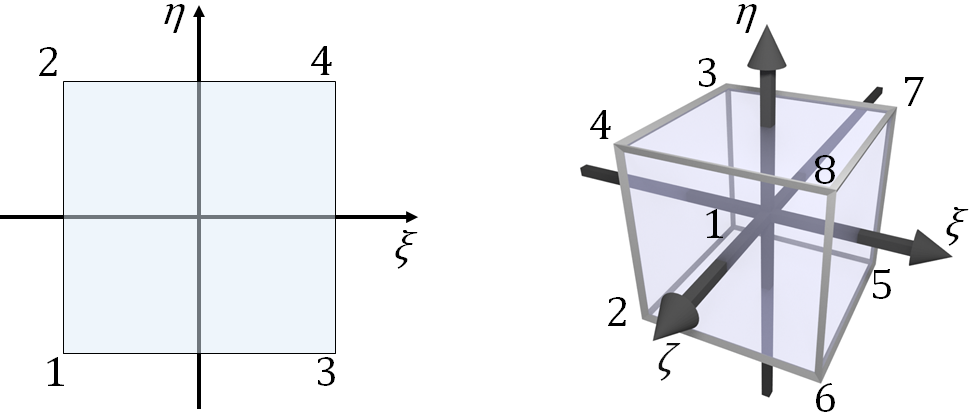
\includegraphics[width=0.8\textwidth]{figs/refEle.png}
\caption{Standard elements for 2D quadrilateral (left) 
	and 3D hexahedral elements (right). The standard element spans $[-1,1]$ in each axis
	to facilitate Gaussian quadrature rules. Nodes are marked with their indices.
	}
\label{fig:standardEle}
\end{figure}
\begin{table}
	\begin{center}
		\begin{tabular}{ |c| r r r|}
			\hline
			Index & $\xi_i$ & $\eta_i$ & $\zeta_i$ \\ \hline
			1 & -1 & -1 & -1\\  
			2 & -1 & -1 & 1\\
			3 & -1 & 1 & -1\\  
			4 & -1 & 1 & 1\\
			5 & 1 & -1 & -1\\  
			6 & 1 & -1 & 1\\
			7 & 1 & 1 & -1\\  
			8 & 1 & 1 & 1\\
		\hline						
		\end{tabular}
	\end{center}
	\caption{Nodal positions of the standard hexahedron element in the natural coordinates.
		Coincidentally, these coordinate values can also be used to define the trilinear interpolation weights.}
	\label{tab:natCoord}
\end{table}

With the interpolation function fully defined in the natural coordinates, 
we can use it to map a point $\chi$ in natural coordinates to a point
$\mathbf{X}$ inside a general hexahedron element with nodal positions $\mathbf{X}_i$ as follows
\begin{equation}
	\mathbf{X}=\sum_i N_i(\chi)\mathbf{X}_i.
	\label{eq:rest}
\end{equation}

Note here we are interpolating a vector-valued function where each coordinate is interpolated independently.
\subsection{Modeling Elastic Objects}
Elastic objects tend to return to its rest shape when deformed by external forces such as stretching, bending, twisting etc. The direction and strength of the tendency to restore to its rest shape is described by its elastic forces.
To model the exact behavior of a small piece of material,
we first use finite elements to approximate its deformations.
A hexahedron element models a piece of elastic material that can deform by changing its nodal positions.
The internal volume deforms by following the nodal displacements using trilinear interpolation.
Of course real materials do not have to deform this way.
The trilinear interpolation is only an approximation.
More precisely, for an element with a rest configuration given by $\mathbf{X}_i$,
its nodes can be moved to new positions $\mathbf{x}_i$ by displacements $\mathbf{u}_i$,
i.e., $\mathbf{x}_i=\mathbf{X}_i+\mathbf{u}_i$.
For any point $\mathbf{X}$ inside the element with known natural coordinates $\chi$, its displacement $\mathbf{u}(\mathbf{X})$ is given by interpolation
\begin{equation}
\mathbf{u}(\mathbf{X}) = \sum_iN_i(\chi)\mathbf{u}_i.
\label{eq:disp}
\end{equation}
To make a clear distinction between $\mathbf{X}$ and $\mathbf{x}$,
$\mathbf{X}$ is defined as a point in the \textbf{reference space} that represents the undeformed shape of an object. The lower case $\mathbf{x}$ lives in the \textbf{deformed space} that represents the deformed configuration of an object.

From now on, to simplify notation, $N_i(\xi)$ will be written as $N_i$.
The deformation of an object is quantified using strain measures,
which is defined in terms of the difference in displacement between nearby points.
Intuitively, if $\mathbf{u}(\mathbf{X})$ is constant, then the displacement field is just a translation. In this case the material is undeformed and should not contain any strain.
More generally, the difference of displacement between nearby points can be written using derivatives,
\[
\mathbf{F}=\frac{\partial \mathbf{u}}{\partial \mathbf{X}}+\mathbf{I}
=\begin{pmatrix}
\dfrac{\partial u_1}{\partial X_1} & \dfrac{\partial u_1}{\partial X_2}&\dfrac{\partial u_1}{\partial X_3}\\
\dfrac{\partial u_2}{\partial X_1} & \dfrac{\partial u_2}{\partial X_2}&\dfrac{\partial u_2}{\partial X_3}\\
\dfrac{\partial u_3}{\partial X_1} & \dfrac{\partial u_3}{\partial X_2}&\dfrac{\partial u_3}{\partial X_3}\\
\end{pmatrix}+\mathbf{I}.
\]
The matrix $\mathbf{F}$ is the \textbf{deformation gradient} and $\mathbf{I}$ is the identity matrix.
While we do not have a closed-form expression of $\mathbf{u}$ written in terms of $\mathbf{X}$,
we have Equation~\ref{eq:rest} and~\ref{eq:disp} that relate $\mathbf{u}$ and $\mathbf{X}$ through $\chi$.
The term $\frac{\partial \mathbf{u}}{\partial \mathbf{X}}$ can be re-written using the chain rule,
\begin{equation}
\frac{\partial \mathbf{u}}{\partial \mathbf{X}}=
\frac{\partial \mathbf{u}}{\partial \chi}
\frac{\partial \chi}{\partial \mathbf{X}}=
(\sum_i\mathbf{u}_i\frac{dN_i}{d\chi})(\frac{\partial \mathbf{X}}{\partial \chi})^{-1}
\label{eq:dudX}
\end{equation}
The matrix $\frac{\partial \mathbf{X}}{\partial \chi}$ is called the Jacobian matrix of $\mathbf{X}$ with respect to $\chi$ and is written as
\[
\mathbf{J}=\frac{\partial \mathbf{X}}{\partial \chi}
= \sum_i\mathbf{X}_i\frac{dN_i}{d\chi}.
\]
By convention, $\frac{dN_i}{d\chi}$ is a $1\times 3$ row vector.
The term $\mathbf{X}_i\frac{dN_i}{d\chi}$ is an outer product that produces a $3\times 3$ matrix.

Given the full expression for the deformation gradient $\mathbf{F}$, we can now define elastic energy densities. 
The elastic energy density function $\Psi(\mathbf{F})$ computes a non-negative energy value given a deformation gradient.
This function fully defines the elastic behavior of a piece of material especially the elastic forces.
Integrating $\Psi$ over the domain $\Omega$ of an element in the reference space yields the total elastic energy contained by that element.
\[
E(\mathbf{x}_1,...,\mathbf{x}_8)=\int_{\Omega}\Psi dV.
\]
Differentiating $E$ with respect to nodal positions $\mathbf{x}_i$ gives us the opposite direction of nodal elastic forces
\[
-\mathbf{f}_i=\frac{dE}{d\mathbf{x}_i}=\int_{\Omega}
\frac{d\Psi(\mathbf{F})}{d\mathbf{F}}
\frac{d\mathbf{F}}{d\mathbf{x}_i}dV
=\int_{\Omega}
\mathbf{P}(\mathbf{F})
\frac{d\mathbf{F}}{d\mathbf{x}_i}dV,
\]
Where
\[
\mathbf{P}(\mathbf{F})=\dfrac{d\Psi(\mathbf{F})}{d\mathbf{F}}.
\]
$\mathbf{P}(\mathbf{F})$ is called the fist Piola-Kirchhoff stress.
It transforms a normal vector in the reference space to a force acting in the deformed configuration divided by area in the reference space.
Integrating in the reference space is not easy since the element is not necessarily a rectangular shape. By change of variables, we can integrate in natural coordinates
in the set $\Omega_{\chi}=[-1,1]^3$.
\begin{align*}
\int_{\Omega}
\mathbf{P}(\mathbf{F})
\frac{d\mathbf{F}}{d\mathbf{x}_i}dV
&=\int_{\Omega_{\chi}}
\mathbf{P}(\mathbf{F})
\frac{d\mathbf{F}}{d\mathbf{x}_i}|\det{\mathbf{J}}|dV\\
&=\int_{\Omega_{\chi}}
\mathbf{P}(\mathbf{F})\mathbf{J}^{-T}
\frac{dN_i}{d\chi}\det{\mathbf{J}}\,dV.
\end{align*}
Here we dropped the absolute value sign because the undeformed element is required to have positive determinant everywhere.
To numerically evaluate the integral, we use Gaussian quadrature rules.
For example, the two-point Gaussian quadrature rule places quadrature points at
$\pm \sqrt{\frac{1}{3}}$ in natural coordinates, which results in $8$ quadrature points with equal weights in 3D.
For each quadrature point $j$, we evaluate the integrand and multiply by the quadrature weight $w_j$. The integral is written as a summation
\[
-\mathbf{f}_i=\sum_j w_j\mathbf{P(\mathbf{F}_j)}\mathbf{J}^{-T}
\frac{dN_i}{d\chi}\det{\mathbf{J}}.
\]

$\Psi$ determines the constitutive model of elasticity, i.e. the relationship between strain measures and stress.
This thesis primarily uses two kinds of constitutive models: linear elasticity and Neo-Hookean model. For the linear elasticity, we first define the infinitesimal strain tensor
\[
\epsilon = \frac{1}{2}(\mathbf{F}+\mathbf{F}^T)-I.
\]
This strain tensor is a symmetric matrix. The stress tensor derived from this strain measure is also a symmetric matrix. This property is a necessary condition for conservation of linear and angular momentum. 
In other words, stress and internal elastic forces should not cause any change in total linear or angular momentum.
The strain energy density function for isotropic linear elasticity is
\[
\Psi(\mathbf{F}) = \mu\epsilon:\epsilon + \frac{\lambda}{2}tr^2(\epsilon).
\]
$\mu$ is a material parameter called shear modulus and $\lambda$ is Lam\'{e}'s first parameter.
$tr(\epsilon)$ is the trace of the strain tensor.
Differentiate $\Psi$ to obtain
\[
\mathbf{P}(\mathbf{F})=\mu(\mathbf{F}+\mathbf{F}^T-2\mathbf{I})+\lambda tr(\mathbf{F}-\mathbf{I})\mathbf{I}.
\]
For anisotropic linear elasticity, the constitutive equation is written as
\begin{equation}
\sigma=\mathbf{C}\epsilon,
\label{eq:constitutive}
\end{equation}
where $\sigma$ is the $3\times 3$ Cauchy stress tensor, $\mathbf{C}$ is a
fourth-order $3\times 3\times3\times3$ tensor called the tensor of elasticity.
The term $\mathbf{C}\epsilon$ is a summation of component-wise products.
In Einstein notation,
\[
\sigma_{ij}=C_{ijkl}\epsilon_{kl}.
\]
Cauchy stress relates to the first Piola-Kirchhoff stress by
\[
\sigma = \frac{1}{\det \mathbf{F}}\mathbf{P}\mathbf{F}^T
\]
The corresponding strain energy density function is
\[
\Psi(\epsilon)=\frac{1}{2}\mathbf{C}\epsilon^2.
\]
To simplify notations, the stress and strain tensors are written as vectors instead of matrices.
Using Voigt notation,
a stress tensor of the form
\[
\sigma=\begin{pmatrix}
\sigma_{xx} & \sigma_{xy} & \sigma_{xz}\\
\sigma_{yx} & \sigma_{yy} & \sigma_{yz}\\
\sigma_{zx} & \sigma_{zy} & \sigma_{zz}
\end{pmatrix}
\]
is rewritten as
\[\sigma=(\sigma_{xx} , \sigma_{yy} , \sigma_{zz},
\sigma_{xy} , \sigma_{yz} , \sigma_{zx}).
\]
This allows the tensor of elasticity to be written as a $6\times 6$ matrix.
For orthotropic linear materials, $\mathbf{C}$ takes the following form
\[
\mathbf{C}=
\begin{pmatrix}
C_{1111} & C_{1122} & C_{1133} & 0 & 0 & 0 \\
 & C_{2222} & C_{2233} & 0 & 0 & 0 \\
& & C_{3333} & 0 & 0 & 0 \\
& & & C_{1212} & 0 & 0 \\
 & Symm &  & & C_{2323} & 0 \\
 & & & & & C_{1313}
\end{pmatrix}.
\]
For a more restricted subset of materials with cubic symmetry, 
$\mathbf{C}$ is specified by three material parameters: Young's modulus $E$,
Poisson's ratio $\nu$, and shear modulus $G$ or $\mu$.
\[\mathbf{C}=
\begin{pmatrix}
(1-\nu)\hat{E} & \nu\hat{E} & \nu\hat{E} & 0 & 0 & 0 \\
&(1-\nu)\hat{E} & \nu\hat{E} & 0 & 0 & 0 \\
& &(1-\nu)\hat{E} & 0 & 0 & 0 \\
& & & \mu & 0 & 0 \\
& Symm &  & & \mu & 0 \\
& & & & & \mu
\end{pmatrix},\hat{E} = \frac{E}{(1-2\nu)(1+\nu)}.
\]

The advantage of the linear elasticity is that it assumes a linear relationship between stress and strain. This leads to a linear relationship between nodal displacements and nodal forces
as follows
\[
\mathbf{K}\mathbf{U}=-\mathbf{f}.
\]
Here $\mathbf{K}$ is called the stiffness matrix given by
\[
\mathbf{K}=\frac{\partial^2 \Psi}{\partial\mathbf{U}^2}.
\]
$\mathbf{U}$ is the concatenated nodal displacement vector
$[\mathbf{u}_1,\mathbf{u}_2,...,\mathbf{u}_8]$ and $\mathbf{f}$ is the concatenated internal nodal force vector.
Computing the deformation under external boundary conditions and forces requires only a single linear solve
\[
\mathbf{U}=\mathbf{K}^{-1}\mathbf{f}_{ext},
\]
given sufficient boundary conditions.
The stiffness matrix is sparse and positive semi-definite (positive definite with enough constraints).
A wide class of linear solvers have been developed for such linear systems.
To see the linear relationship between displacements and force,
we just need to derive the linear relationship between $\epsilon$ and $\mathbf{u}_i$
from Equation~\ref{eq:dudX} and combine it with Equation~\ref{eq:constitutive}.
For a point $\mathbf{X}\in\mathbb{R}^3$, we will use superscripts to denote its individual coordinates.
Define the strain-displacement matrix
\[
\mathbf{B}(\mathbf{X})=
\begin{pmatrix}
\dfrac{dN_1}{d\mathbf{X}^1} & 0 & 0 & ... \\
0 & \dfrac{dN_1}{d\mathbf{X}^2} & 0 & ... \\
0 & 0 & \dfrac{dN_1}{d\mathbf{X}^3} & ... \\
\dfrac{dN_1}{d\mathbf{X}^2} & \dfrac{dN_1}{d\mathbf{X}^1} & 0 & ... \\
0 & \dfrac{dN_1}{d\mathbf{X}^3} & \dfrac{dN_1}{d\mathbf{X}^2} & ... \\
\dfrac{dN_1}{d\mathbf{X}^3} & 0 & \dfrac{dN_1}{d\mathbf{X}^1} & ...
\end{pmatrix}.
\]
For an eight-node hexahedron, this matrix has $3\times 8=24$ columns.
This matrix computes the strain tensor at a point $\mathbf{X}$ given nodal displacements
\[
\epsilon(\mathbf{X})=\mathbf{B}(\mathbf{X})\mathbf{U}.
\]
This linear relationship concludes our claim that linear elasticity model defines a linear relationship between nodal displacements and nodal forces.
Further, using quadrature rules, we can numerically evaluate $\mathbf{K}$ as
\[
\mathbf{K}=\sum_j w_j \mathbf{B}(\mathbf{X}_j)\mathbf{C}\mathbf{B}(\mathbf{X}_j)\det \mathbf{J}.
\]

The downside of linear elasticity is that it does not handle rotation properly.
An elastic object undergoing a rigid rotation should contain zero elastic energy.
If we let $\mathbf{F}=\mathbf{R}$ for some rotation matrix $\mathbf{R}$,
the resulting energy measure is generally non-zero.
This constitutive model is useful only when the deformation is small with respect to the overall size of the object.
When an object undergoes buckling with many potential static equilibrium configurations,
linear elasticity always predict a single solution with little buckling since its elastic energy landscape is convex with a unique local minimum.
Additionally, linear elasticity does not preserve volume according to the Poisson's ratio parameter. In fact, elements can easily invert into non-physical states.

To address the rotation problem, non-linear elasticity models such as the corotated linear elasticity model and the Saint-Venant Kirchhoff model are developed to be rotation invariant.
However, these models still allow an element to invert and do not preserve volume.
We use the Neo-Hookean material model for non-linear elasticity. It resists inverting, and approximately preserves volume according to Poisson's ratio.
The strain energy density of Neo-Hookean model is
\[
\Psi(\mathbf{F})=\frac{\mu}{2}(I_1-3) - \mu \log \det \mathbf{F} 
+ \frac{\lambda}{2}(\log \det \mathbf{F})^2,
\]
where the first isotropic invariant is 
\[
I_1=tr(\mathbf{F}^T\mathbf{F}).
\]
The first Piola-Kirchhoff stress is
\[
\mathbf{P}(\mathbf{F})=\mu(\mathbf{F}-\mathbf{F}^{-T})+\lambda(\log\det\mathbf{F})\mathbf{F}^{-T}.
\]
\section{Data-Driven Coarsening}
Objects with high-resolution, heterogeneous elastic materials are everywhere:
from the output of multimaterial 3D printers to virtual characters 
gracing the screen in our summer blockbusters.
Designing such objects is made possible by the tight coupling of design
tools and numerical simulation which allows designers or automatic
algorithms to update geometry or material parameters and subsequently
estimate the physical effects of the change.
Fast, accurate simulation techniques that can handle runtime changes in geometry
and material composition are a necessity for such iterative design algorithms.
There have been a large number of works on speeding up FEM simulations,
and these speed improvements have enabled FEM to be used in many performance critical tasks 
such as computer animation, surgical training, and virtual/augmented reality.
Even though techniques such as model reduction or numerical coarsening can
achieve order-of-magnitude performance increases,
they require expensive precomputation phases, typically on the order of minutes for large meshes.
This precomputation requires knowledge of an
object’s geometry and material composition a priori, something
that is not known during a design task.
When the user updates the model by changing the geometry or the material distribution,
the preprocessing step must be run again.
As shown in Figure~\ref{fig:typical}a, since this step is inside the design loop,
the user cannot get rapid feedback on the changes made to the object.
\begin{figure}
	\centering
	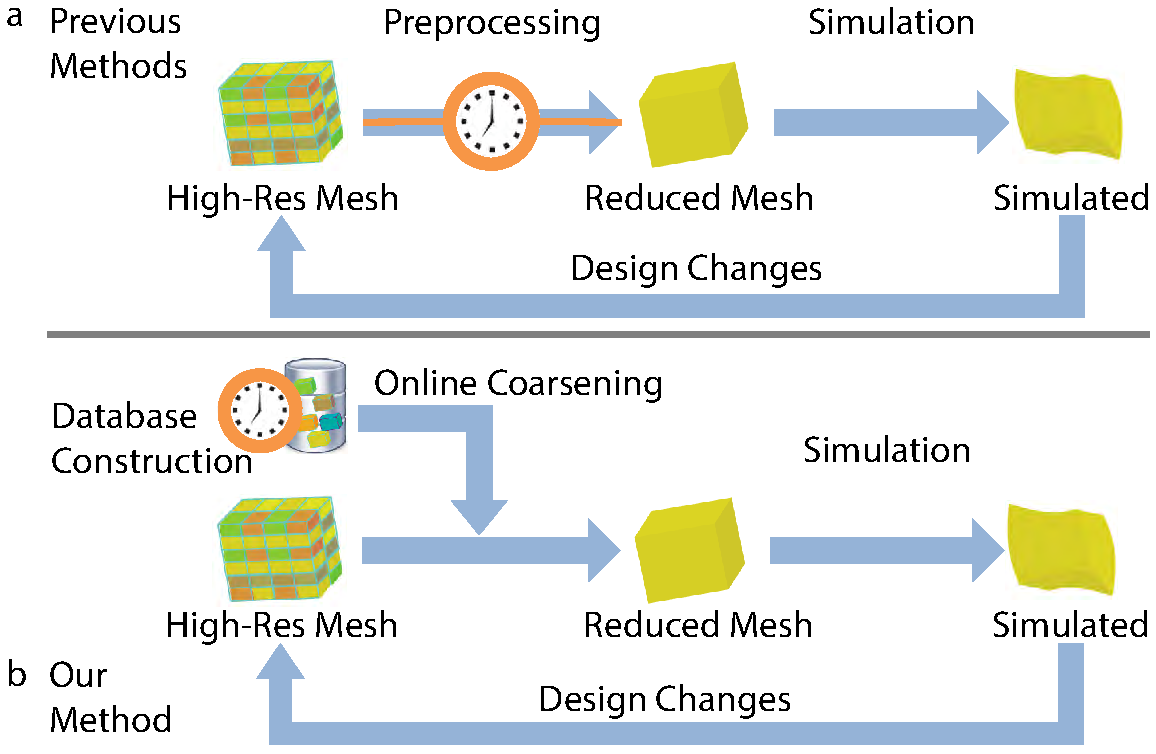
\includegraphics[width=0.8\textwidth]{figs/typical1.pdf}
	\caption{(a) In a typical method, the preprocessing step is offline,
		making the design loop slow. (b) In our method, we move the timeconsuming
		offline computation outside of the design loop.}
	\label{fig:typical}
\end{figure}

We propose Data-Driven FEM (DDFEM), a new simulation methodology
that removes these limitations and is thus extremely well suited
to the types of design problems discussed above.
We divide an object into a set of deformable voxels using embedded finite
elements and coarsen these voxels hierarchically.
A custom metamaterial database is populated with materials that minimize the error incurred by coarsening.
This database is learned once in a completely offline fashion and depends only on the set of materials to be used by the deformable object and not on the actual material distribution
and geometry.
At runtime we use the database to perform fast coarsening of an FEM mesh in a way that is agnostic to changes in geometry and material composition of the object.
The key features of the algorithm are its ability to handle arbitrary, nonlinear elastic
constitutive models as well as to avoid expensive precomputation
within the design loop (Figure~\ref{fig:typical}b).
DDFEM is the first algorithm optimized for interactive design of non-linear elastic objects.

DDFEM is a combination of embedded finite elements and hierarchical
coarsening.
In the remainder of this section, we discuss the problem of coarsening
and introduce the notion of a material palette. We conclude by
summarizing the two main stages of DDFEM—offline coarse material
construction and online coarsening.
\paragraph{Coarsening for finite elements}
The key component of our DDFEM is coarsening.
Coarsening reduces the number of vertices in a finite element simulation mesh in order to improve
runtime performance.
Since simply removing vertices can greatly reduce
the accuracy of the simulation, coarsening schemes also assign
new materials to coarsened elements to minimize this effect.
We regard the global coarsening of a simulation mesh as the result
of many local coarsening operations which map from contiguous
subsets of fine elements with applied materials to coarse elements
with new, optimized materials. Our goal is to precompute these
optimized materials so that coarsening is fast at runtime. Below we
discuss how to make such a precomputation tractable beginning with
our choice of finite element simulation methodology.
\paragraph{Conforming vs. embedded finite elements}
The defining feature of conforming finite element methods is that the simulation
mesh is aligned with the geometry of the object being simulated.
One obvious feature of conforming meshes is that the mesh itself is a
function of the input geometry.
This means that the output of a local coarsening operator (the coarsened mesh) will also be a function
of the input geometry.
Also, the new material computed by each local coarsening operator will be a function of input geometry.
This dependence on input geometry is a significant issue to overcome
if we wish to precompute coarsened materials because, in design
problems, the input geometry is in constant flux.
The number of precomputed coarse materials now depends on the local material
assignment on the simulation mesh and the input geometry.
Thus space of coarsened materials is prohibitively large.
To mitigate this we turn to embedded finite elements.
These methods embed the geometry to be simulated into the simulation mesh with no regard
for whether the mesh conforms to the geometry or not.
Thus an identical simulation mesh can be used for any input geometry.
Local coarsening operations on the embedded mesh yield identical coarse
elements and the optimized coarse material depends only on the
local material distribution on the simulation mesh. This significantly
reduces the size of the coarsened material space. In this paper we
embed all simulation geometry into a hexahedral simulation mesh.
\paragraph{Material palette} We further shrink the space of coarsening operators
using an observation about material design. Designers do
not work in a continuous space of materials but limit themselves to
a relatively compact set (e.g. rubber, wood, steel) related to their
problem domain. We call these discrete sets of materials
palettes and denote them $\mathcal{P}=\{\mathcal{M}^1,...,\mathcal{M}^n\}$.
Here $\mathcal{M}^i$ denotes a specific material model in $\mathcal{P}$, 
and $n$ is the size of the material palette.
In this work we limit ourselves to nonlinear hyper-elastic materials,
which means that each $\mathcal{M}^i$ can be represented by a strain
energy density function.
We also include a void (or empty) material in every palette.
This allows us to perform topology changes in the
same manner in which we perform material assignment updates.
\paragraph{Algorithms}
With the material palette in hand, we can now define our algorithm, which is divided into two distinct phases: an \textbf{offline database construction} stage and an \textbf{online coarsening} stage.  Below we detail the input, output, and steps of each stage:
\vspace{1mm}
\hrule
\textbf{Offline Database Construction}
\vspace{1mm}
\hrule
\begin{compactitem}
	\item \textbf{INPUT:} A palette of materials to be applied to high-resolution hexahedral simulation meshes $\set{P}^0$
	\item \textbf{OUTPUT:} A new palette of coarse elements, $\set{P}^1$, and a mapping from fine material combinations to the coarsened materials in $\set{P}^1$. 
	\item \textbf{STEPS:}
	\item \textbf{FOR EACH} material combination applied to a 2$\times$2$\times$2 cube of high resolution elements
	\subitem $\bullet$ Sample potential energy function of 2$\times$2$\times$2 block
	\subitem $\bullet$ Fit coarse hexahedral element material parameters
	\subitem $\bullet$ Add coarse element to $\set{P}^1$ using high resolution 
	\subitem material IDs as database key
	\item \textbf{END}
\end{compactitem}
\vspace{1mm}
\hrule
\vspace{1mm}
\hrule
\textbf{Online Coarsening}
\vspace{1mm}
\hrule
\begin{compactitem}
	\item \textbf{INPUT:} High resolution hexahedral simulation mesh with 
	\subitem material IDs and
	\subitem coarsened hexahedral simulation mesh 
	\item \textbf{OUTPUT:} Material assignments for coarse mesh
	\item \textbf{STEPS:}
	\item \textbf{FOR EACH} 2$\times$2$\times$2 block in the high resolution mesh
	\subitem $\bullet$ Replace with single coarse element
	\subitem $\bullet$ Assign material from $\set{P}^1$ using high resolution 
	\subitem material IDs as database key
	\item \textbf{END}
\end{compactitem}
\vspace{1mm}
\hrule

\paragraph{Hierarchical coarsening}
We stress that both stages of the DDFEM algorithm can be applied hierarchically. Given the first level of coarse materials, $\set{P}^1$, we can construct a material library, $\set{P}^2$, for the second level by using $\set{P}^1$ as an input material palette. At runtime, the coarsening algorithm looks up materials from $\set{P}^2$ to replace each 2$\times$2$\times$2 coarse block with a single element.

Having introduced the broad strokes of the DDFEM scheme, we move on to a detailed explanation of each algorithmic component. First we discuss database construction in \autoref{sec:database}, followed by the runtime component in \autoref{sec:runtime}. We end by demonstrating the speed and accuracy of DDFEM in \autoref{sec:result}.

\section{Coarse Material Database Construction}
\label{sec:database}
We construct our coarse material database using a potential energy fitting approach.
This is valid due to the hyperelastic materials that make up our material palettes.
Material fitting considers 2$\times$2$\times$2 blocks of high-resolution hexahedral elements (denoted $\set{E}^0$).
For each element $E_k^0\in \, \set{E}^0$, its material is referred to as $\set{M}_k^0\in \, \set{P}^0$. 
Note that $\set{E}$ refers to a set of elements and $E$ refers to a single element.
Given $\set{E}^0$, we can sample its deformation space, and using $\set{M}_k^0$, compute the potential energy $V^0$ for each sample.
Now we must find a coarse material model that, when applied to a single coarse element $\mathit{E}^1$ best approximates $V^0$.
This is accomplished by fitting a coarse potential energy function , $V^1$, to the set of deformation/energy samples.
The fitted energy is stored in the coarse material database and indexed by the material indices of $\set{M}^0$.

\subsection{Coarse Material Model}
Our fitting approach depends on choosing a good coarse material model.
The general hyperelastic material model for a finite element with degrees of freedom $\mathbf{\vr{u}}$
can be represented as an energy function $V(\vr{u},\vr{p})$ parameterized by $\vr{p}$.
For an eight-node hexahedron element, $\vr{u}$ is a $24\times 1$ column vector of nodal displacements
$\vr{u}=(u_{1,x}, u_{1,y},u_{1,z}...,u_{8,x}, u_{8,y},u_{8,z})^T$.
The energy function has to comply with many requirements to be physically meaningful~\cite{Marsden2012}.
Here we list some important requirements:
\begin{enumerate}
	\item Invariance under rigid transformation. Given any block-diagonal rotation matrix $\vr{R}$ composed of
	$3\times 3$ identical rotation matrices, and any translation vector $\vr{d}$,
	\[
	V(\vr{u},\vr{p}) = V( (\vr{R}-\vr{I})\vr{X}+\vr{R}\vr{u}+\vr{d},\vr{p}).
	\]
	\item Tendency to return to the rest shape.
	To implement this feature, the energy function must have a global minimum of
	$V(\vr{u},\vr{p})=0$ at $\vr{u}=\vr{0}$ up to rigid transformations.
	\item Stress increases with strain. This is not always true for heterogeneous materials 
	with internal buckling under load such as foams (polymer plus void).
	For our experiments however, we assume the coarse elements do not undergo deformation large enough to cause internal buckling.
	\item Conservation of momentum. The elastic forces given by
	$\dfrac{DV}{D\vr{u}}$ must not alter the linear and angular momentum of the element.
\end{enumerate}
These seemingly intuitive requirements are difficult to satisfy for functions written in
terms of $\vr{u}$.
For example, here is a simple energy function
\[
V(\vr{u},\vr{p})=\|\vr{u}-\vr{X}\|^2.
\]
This function violates rules 1,3 and 4.
To improve, one can define an energy function by attaching an elastic spring
between every pair of nodes.
This energy function satisfies rules 1 and 4 but violates rule 2 and 3.
To see this, let $\vr{u}=-2\vr{X}$ and check that
the function has the same value for an inverted element.

In order to ensure that our model meets the criteria for a valid energy function, we choose our coarse material model for $\mathit{E}^1$ as a combination of the base material models $\set{M}_k^0$:
\begin{align}
V^1(\vr{u}^1, \, \vr{p}^1) = \sum_{k=1}^8 w_k \, V_k^0(\vr{u}_k^0, \, \vr{p}_k^1, \, \vr{X}_k^1),
\label{eq:materialModel}
\end{align}
where $V_k^0$ is the strain energy density of $\set{M}_k^0$ at quadrature point position $\vr{X}_k^1$ (\autoref{fig:coarseFine}). Here $\vr{u}^1$ is the vector of nodal displacements associated with $\mathit{E}^1$ while $\vr{u}_k^0$ are displacements for the $k^{th}$ element at level $0$ reconstructed using trilinear interpolation from $\vr{u}^1$.
The coarse materials $\vr{p}^1=(\vr{p}_1^1,...,\vr{p}_k^1)$ consists of the stacked material parameter vectors for each base material in $\set{M}_k^0$, themselves denoted by $\vr{p}_k^1$.  $w_k$ is the standard Gaussian quadrature weight.
\begin{figure}
	\centering
	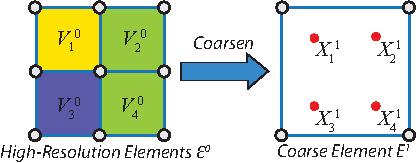
\includegraphics[width=0.6\textwidth]{images/coarseFine.pdf}
	\caption{The relationship between high-resolution and coarsened elements. At each quadrature point $\vr{X}_k^1$, the coarse element copies the corresponding energy density function $V_k^0$ from the high-resolution element.}
	\label{fig:coarseFine}
\end{figure}
We observe that even if the individual base material models are isotropic, the coarse element can become anisotropic by assigning different material parameters at the quadrature points.
We propose to improve the fitting by augmenting the coarse material model with an anisotropic term.
The complete model is then given by
\begin{align}
\begin{split}
V^1(\vr{u}^1, \, \vr{p}^1, \, C) &= \sum_{k=1}^8 \bigg( w_k \, V_k^0(\vr{u}^0, \,\vr{p}_k^1, \, \vr{X}_k^1)\\
& + C_k\left( \sqrt{\vr{v}^T\vr{F}_k^T\vr{F}_k\vr{v}} - 1\right)^2\bigg),\\
\label{eq:materialModel2}
\end{split}
\end{align}
where $\vr{v}$ is a unit-length direction of anisotropy and $C_k$ is the scaling parameter at the $k^{th}$ quadrature point. 
The gradient of the anisotropic term is
\[
\frac{d( \sqrt{\vr{v}^T\vr{F}^T\vr{F}\vr{v}} - 1)^2}{d\mathbf{F}}
=(1-\frac{1}{\|\mathbf{F}\mathbf{v}\|})\mathbf{F}\mathbf{v}\mathbf{v}^T.
\]
The second order gradient in the direction of a given $\delta \mathbf{F}$ is
\[
\left((1-\frac{1}{\|\mathbf{F}\mathbf{v}\|})\mathbf{I} 
+ \frac{1}{\|\mathbf{F}\mathbf{v}\|^3}\vr{F}\vr{v}\vr{v}^T\vr{F}^T\right)\delta\mathbf{F}^T\mathbf{v}\mathbf{v}^T.
\]
\subsection{Force Space Sampling}
\label{sec:force_space_sampling}
As mentioned previously, we take a sampling-based approach to coarse material fitting. In order to fit our model (\autoref{eq:materialModel2}) to $V^0$ we first draw a number of samples from the deformation space of $\set{E}^0$ and compute $V^0$ for each sample.
If a user has prior knowledge of the set of meshes and simulations that they will require, then the best way to draw the samples is to run a number of anticipated simulations with various material combinations.
In this paper, we provide a more general method to draw samples for a material model.
Initially, we attempted sampling by applying a random deformation to the corners of $\mathit{E}^1$; however, this led to many infeasible samples for very stiff materials.
In order to alleviate this problem we perform sampling in the force space.

For each element $\mathit{E}^0\in \, \set{E}^0$ we apply a set of randomly generated forces.
We solve an elastostatic problem to compute the deformation of $\set{E}^0$, using constraints to remove rigid motion. Recall that this is fast because $^0\set{E}$ consists of just 8 elements.
Each sample is then a tuple $\left\{\vr{u}^0, \, V^0\right\}$ (\autoref{fig:sampling}) 
where $^0\vr{u}$ are the nodal displacements of $\set{E}^0$,
and $V^0$ is the strain energy density value of this deformed configuration.
\begin{figure}
	\centering
	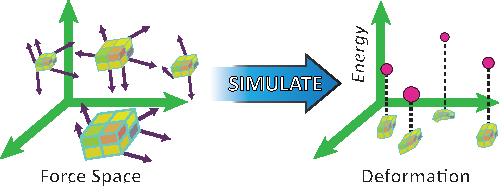
\includegraphics[width=0.6\columnwidth]{images/sampling.pdf}
	\caption{ We sample the energy function of a 2$\times$2$\times$2 block of hexahedra by applying random forces and deforming the block using FEM. Each set of forces results in a deformation-energy tuple which is used during fitting.}
	\label{fig:sampling}
\end{figure}

\subsection{Fitting}
\label{sec:fitting}
Given a set of deformation samples, $\left\{ \vr{u}^0, \,V^0\right\}$, we perform a non-negative least squares fit to determine the parameters, $\vr{p}^*$, for material model(\autoref{fig:fitting}):
\begin{align}
\vr{p}^*= \underset{\vr{p}^1}{\operatorname{argmin}} \, \sum_{s=1}^{n_s}\left(V_s^0- \, V^1\left(\vr{r}\left(\vr{u}_s^0\right), \, \vr{p}^1\right)\right)^2,
\label{eq:fitting}
\end{align}
where $\vr{r}$ constructs $\vr{u}^1$ from $\vr{u}^0$, $n_s$ is the total number of samples, and $s$ indexes all samples. In our experiments we use the simplest form of $\vr{r}$ choosing it to extract the displacements of the corners of $\set{E}^0$.
The material parameters are all constrained to be positive to improve simulation stability.
Since the material parameters have physical meanings such as Young's modulus and spring stiffness,
the non-negativity constraint specifies that the coarse material is made of traditional base materials.

\paragraph{Fitting in the Presence of Anisotropy}
If performed naively this optimization is nonlinear because we must simultaneously solve for $\vr{v}_k$, the preferred direction of anisotropy. This can severely slow the fitting procedure, especially in cases where it would otherwise be a linear least squares problem (i.e if all fine-scale materials are Neo-Hookean or a similarly simple material model).
To avoid this problem we first estimate all anisotropy directions, and then solve \autoref{eq:fitting} for the remaining material parameters.
Our intuition is that anisotropy manifests itself as preferential stretching along a particular axis. To find this axis, we apply stretching forces to a block in a discrete set of directions uniformly sampled over a sphere.
If the stretching force is close to the direction of anisotropy, then the amount of stretching deformation is reduced.
For any given stretching direction $\mathbf{v}$, we apply a stretching force and compute the deformation gradient $\mathbf{F}$ of  each quadrature point.
Under $\mathbf{F}$, a unit length vector in direction $\mathbf{v}$ is stretched to a new length $l = \|\mathbf{F}\mathbf{v}\|$.
The set of all 3D vectors $l\mathbf{v}$ forms an ellipse-like shape.
We find the principal axes of the ellipse (via SVD) and use them as directions of anisotropy.
\begin{figure}
	\centering
	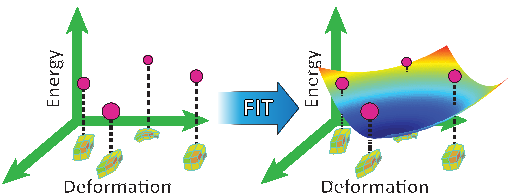
\includegraphics[width=0.6\columnwidth]{images/fitting.pdf}
	\caption{ Coarse potential energy functions are fitted to the deformation-energy samples using a least-squares optimization.}
	\label{fig:fitting}
\end{figure}
\paragraph{Regularization} Since vastly different material assignments, $^0\set{M}_k$, can produce the same coarse material, our na\"{i}ve cost function (\autoref{eq:fitting}) can produce very large parameter values and even non-physical negative ones.
For example, consider a homogeneous material assignment at the high-resolution level.
The same coarse material can be achieved by interleaving hard and soft materials at each fine element or by assigning a single, well chosen material to all fine elements.
To overcome this, we add a regularization term to control the parameter ranges and prevent overfitting of the training samples.
Our modified error function takes the following form:
\begin{equation}
\sum_{s=1}^{n_s}\left(V_s^0- \, V^1\left(\vr{r}\left(\vr{u}_s^0\right), \, \vr{p}^1\right)\right)^2 + 
\lambda\sum_k (\vr{p}_k^1 - \, \vr{p}_k^0)^2,
\end{equation}
which prevents material parameters from deviating too far from  $\set{M}_k^0$.
We chose the regularization constant $\lambda=0.02$ for the results in this paper.
In our experiments, since the base energy functions are linear with respect to the material parameters, the fitting problem can be solved by linear regression with regularization.

\begin{figure}
	\centering
	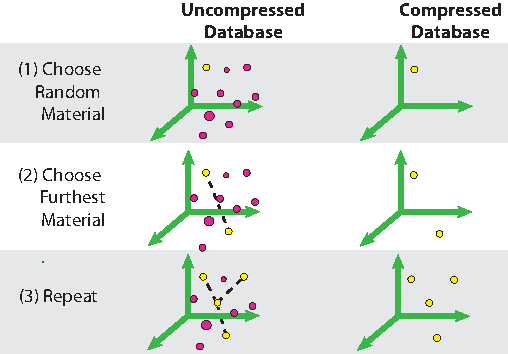
\includegraphics[width=0.6\columnwidth]{images/compression}
	\caption{Database compression step adds coarse materials to a compressed database by a farthest point sampling strategy.}
	\label{fig:compression}
\end{figure}

\subsection{Database Compression}
\label{sec:compression}
Given $n$ materials in the palette, the number of material combinations in a 2$\times$2$\times$2 block is $n^8$. In modern hardware, it is impossible to compute and store all material combinations even for a moderately-sized palette with $100$ materials.
In order to compress the number of materials stored in our coarse material database, we select a small number of representative material combinations and remove all others. We compare materials in a feature space. In order to construct coarse material feature vectors, we first select a common subset of deformations from all computed deformation samples. We then evaluate the potential energies of each coarse material at each deformation sample. The stacked vector of energies becomes a coarse material feature vector. 

Since our base materials differ in stiffness by orders of magnitude, we take the logarithm to measure the difference in ratio.
Let $D$ be the $L^2$ norm of log-energies between the two materials given by
\begin{equation}
D(A,B)=\sqrt{\sum_s (\log(V^{A}_{s})-\log(V^{B}_{s}))^2},
\end{equation} where $A$ and $B$ denote two distinct coarse materials in the database. 
Given the distance metric, we can select $k$ representatives materials using farthest point sampling~\cite{eldar1997farthest}. We randomly choose an initial coarse material and then repeatedly select the material combination furthest away from any previous representatives -- continuing until we obtain $k$ representatives (\autoref{fig:compression}). This compression algorithm chooses $k$ samples that equally cover the coarse material energy space, helping to preserve good behavior in our coarse simulations. 
\subsection{Hierarchical Coarsening}
While one level of coarsening can yield significant speed-ups, DDFEM can also be applied hierarchically.
As discussed in~\autoref{sec:compression}, the exponential growth of coarse material palettes at each level makes it prohibitively expensive to perform fitting.
We address this by changing our coarsening strategy. 
Instead of choosing $\set{E}^0$ to be a 2$\times$2$\times$2 block we choose it to be a 2$\times$1$\times$1 block, which we coarsen. We construct an intermediate database of materials and compress. 
We then choose $\set{E}^0$ to be a 1$\times$2$\times$1 block, coarsen and compress, and finally a 1$\times$1$\times$2 block, coarsen and compress. Intermediate compression greatly reduces the number of samples we need to generate in order to populate the material parameter database for the next coarsening level. 
It is important to note that our intermediate databases only store lookup tables which allow us to extract appropriate material IDs for the next coarsening stage. Material parameters need only be stored in the final database since it is these elements that are simulated.
\begin{figure}
	\centering
	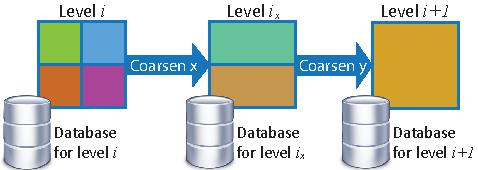
\includegraphics[width=0.7\textwidth]{images/hierchical}
	\caption{Hierarchical coarsening operates on one dimension at a time, performing clustering at each intermediate stage (here denoted $i_x$). This allows our compression algorithm to be applied aggressively, greatly reducing the number of energy samples we need for fitting material parameters. }
	\label{fig:hierarchy}
\end{figure}
\section{Runtime Simulation}
\label{sec:runtime}
Once our coarse material database, $\set{P}^1$, has been constructed we can use it to perform fast online coarsening. 
Initially, the user loads geometry which is embedded in a hexahedral grid for simulation. Prior to simulation we iterate over all 2$\times$2$\times$2 blocks of hexahedral elements and perform mesh coarsening by replacing these 8 elements with a single coarse element. We perform a database lookup into $\set{P}^1$, using the material ID numbers of the 8 original elements, to quickly retrieve the optimal coarse material for this coarse element. Database lookup is fast (even using our unoptimized, single-threaded implementation), and this is what makes DDFEM so appealing.
We achieve significant simulation speed-up from coarsening, retain accuracy in the simulation, and reduce the cost of material coarsening at runtime to a negligible amount.
	Our material model can be used in any simulation algorithm suitable for non-linear elasticity. In our experiments, we use Coin-IpOpt~\cite{ipopt} to implement static and dynamics simulations with tolerance (``tol'' option) set to $0.5$. We use Pardiso as our linear solver.
	For timing purposes, we limit Pardiso to single thread mode.
	The pseudo-code for static simulation is shown in~\autoref{alg:sim}.
\begin{algorithm}
	\caption{Static Simulation}\label{alg:sim}
	\begin{algorithmic}[1]
		\REPEAT
		\STATE $\mathbf{f}$: global force vector
		\STATE $L$: triplet list for global stiffness matrix
		\FOR{each element e}
		\STATE compute elastic force $\mathbf{f}_e$
		\STATE add $\mathbf{f}_e$ to $\mathbf{f}$
		\ENDFOR
		\STATE add external force $\mathbf{f}_{ext}$ to $\mathbf{f}$
		\FOR{each element e}
		\STATE $\mathbf{K}_e$: element stiffness matrix
		\FOR{each quadrature point q}
		\STATE compute stiffness matrix $\mathbf{K}_q$ at quadrature point
		\STATE $\mathbf{K}_e+=\mathbf{K}_q$
		\ENDFOR
		\STATE append entries of $\mathbf{K}_e$ to $L$
		\ENDFOR
		\STATE sort $L$ to get sparse stiffness matrix $\mathbf{K}$
		\STATE set entries in $\mathbf{K}$ and $\mathbf{f}$ for fixed vertices
		\STATE $\Delta\mathbf{x}=\mathbf{K}^{-1}\mathbf{f}$
		\STATE compute step size $h$ using line-search
		\STATE $\mathbf{x}+=h\Delta\mathbf{x}$
		\UNTIL{convergence}
	\end{algorithmic}
\end{algorithm}

\begin{table}[!h]
	\centering
	\footnotesize
	\begin{tabular}{l c r r r r r r r r}
		\hline 
		\textbf{Example} &\textbf{grid size}&\textbf{rel sp}&\textbf{time/iter}&\textbf{iters}&\textbf{error}\\
		\hline
		{\color{HiResColor}Pushing(0)} &16$\times$16$\times$16&1.0 &1.010 &5&-\\
		{\color{DDFEMColor}Pushing(1)} &8$\times$8$\times$8   &11.5&0.087&5&8.91e-4\\
		{\color{DDFEMColor}Pushing(2)} &4$\times$4$\times$4   &31.4&0.032&5&1.36e-2\\
		\hline 
		{\color{HiResColor}Bending(0)} &8$\times$32$\times$8&1.0   &0.270 &28&-\\
		{\color{DDFEMColor}Bending(1)} &4$\times$16$\times$4&12.6  &0.028 & 22& 5.60e-2\\
		{\color{DDFEMColor}Bending(2)} &2$\times$8$\times$2 &22.7  &0.015 & 22&8.88e-2\\
		\hline 
		{\color{HiResColor}Twisting(0)} &8$\times$32$\times$8&1.0  & 0.300 & 16&-\\
		{\color{DDFEMColor}Twisting(1)} &4$\times$16$\times$4&15.2 & 0.031 & 10&1.56e-2\\
		{\color{DDFEMColor}Twisting(2)} &2$\times$8$\times$2 &20.7 & 0.019 & 12&3.28e-2\\
		\hline
		{\color{HiResColor}Buckling(0)} &128$\times$8$\times$16&1.0   &8.85 &32&-\\
		{\color{DDFEMColor}Buckling(1)} &64$\times$4$\times$8  &50.1 &0.28 &20&7.24e-3\\
		{\color{DDFEMColor}Buckling(2) }&32$\times$2$\times$4  &331.8&0.12 &7 &3.14e-2\\
		\hline
		{\color{HiResColor}Fibers(0)} &32$\times$100$\times$32&1.0  &193.85&17&-\\
		{\color{DDFEMColor}Fibers(1)} &16$\times$50$\times$16 &51.2 &4.95  &13& 2.94e-2\\
		{\color{DDFEMColor}Fibers(2)} &8$\times$25$\times$8   &489.5&0.96  &7 & 4.26e-2\\
		\hline
		{\color{HiResColor}Bridge(0)} &56177&1.0&43.44&14&-\\
		{\color{DDFEMColor}Bridge(1)} &9727&8.4&4.88&15&4.39e-3\\
		{\color{HiResColor}Bridge-arch(0)} &65684&1.0&54.99&3&-\\
		{\color{DDFEMColor}Bridge-arch(1)} &11695&8.1&7.84&3&3.68e-4\\
		\hline
		{\color{HiResColor}George(0)} &46152 & 1.0&52.19&23&-\\
		{\color{DDFEMColor}George(1)} &6755 & 16.4&3.49&21&2.86e-2\\
		{\color{HiResColor}George-bone(0)} &46152 & 1.0&41.35&12&-\\
		{\color{DDFEMColor}George-bone(1)} &6755 & 13.2&2.70&14&2.99e-2\\
		\hline
	\end{tabular}
	\vspace{-4pt}
	\caption{Relative performance, absolute performance in seconds and average vertex error relative to the bounding box size for full-resolution and coarsened simulations.
		Relative performance illustrates the performance increase gained by coarsening with respect to the time taken for the high-resolution static simulation to converge. Bracketed numbers after each example name indicate the number of coarsening levels with 0 indicating the {\color{HiResColor}high-resolution} simulation. All computation times are recorded using Coin-IpOpt running in single threaded mode on a 2.5 GHz Intel Core i7 processor. }
	\label{table:performance}
\end{table}
\begin{figure}[t]
	\centering
	\begin{tabularx}{0.92\columnwidth}{ Y Y }
		\textbf{Pushing} & \textbf{Twisting} \\
		\textbf{12x Faster} & \textbf{15x Faster}
	\end{tabularx}\\
	\subcaptionbox{}{
		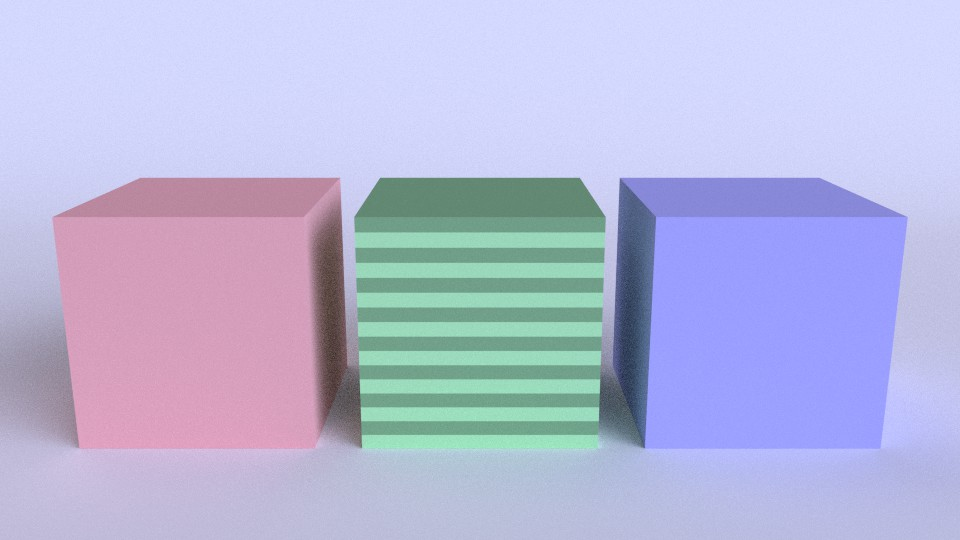
\includegraphics[width=0.45\textwidth]{images/push_l1_begin}
	}%\vrule
	\subcaptionbox{}{
		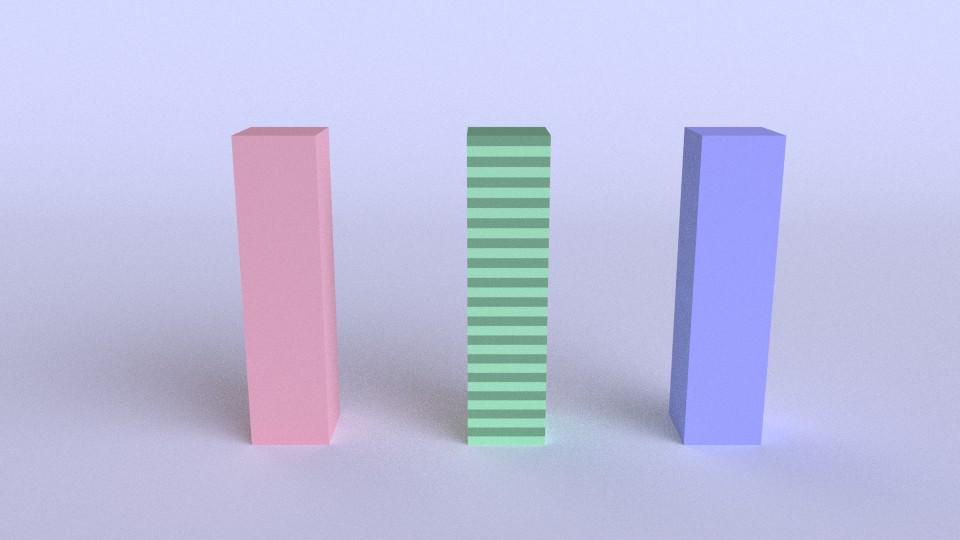
\includegraphics[width=0.45\textwidth]{images/twist_l1_begin}
	}
	\\
	\subcaptionbox{}{
		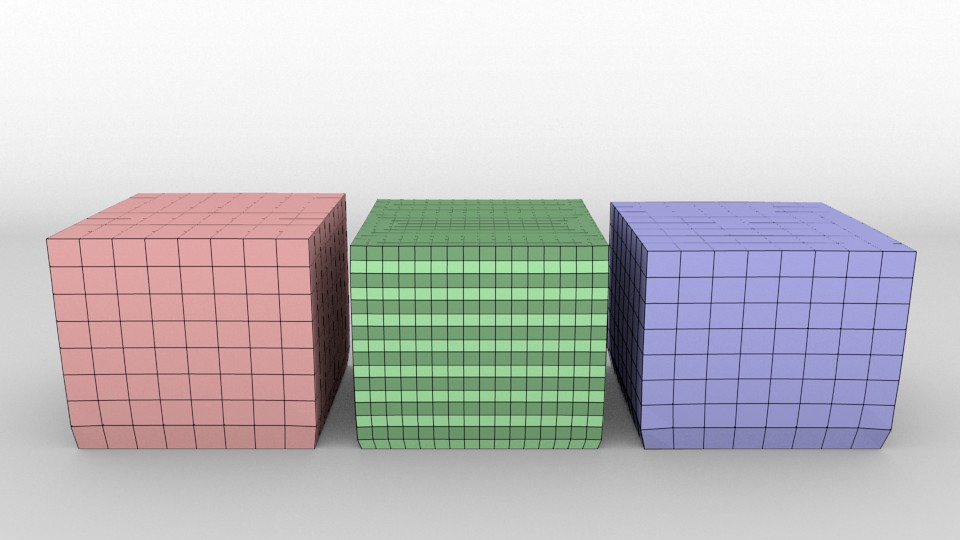
\includegraphics[width=0.45\textwidth]{images/push_l1_wire_end}
	}%\vrule
	\subcaptionbox{}{
		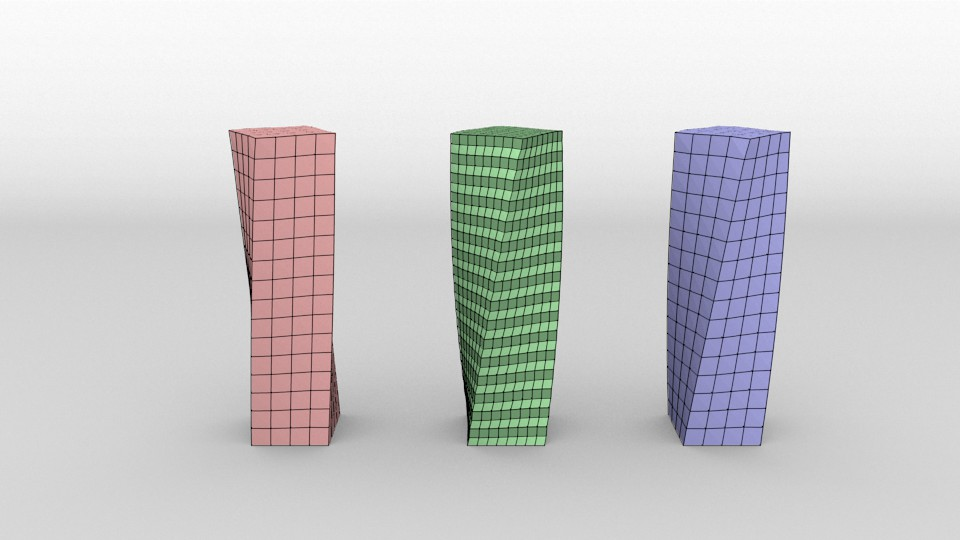
\includegraphics[width=0.45\textwidth]{images/twist_l1_wire_end}
	}
	%\vspace{-3mm}
	\caption{Examples of pushing a cube (a - Initial State, c - Compressed) and twisting a bar (b - Initial State, d - Compressed), both with heterogeneous material distribution. We compare {\DDFEM} to {\Naive} and the  ground-truth, {\HiRes}. We render wire frames to show the simulation meshes.}
	\label{fig:accuracy}
\end{figure}
\begin{figure}[t]
	\centering
	\begin{tabularx}{0.92\columnwidth}{ Y Y }
		\textbf{1 Level of Coarsening} & \textbf{\textbf{2 Levels of Coarsening}} \\
		\textbf{13x Faster} & \textbf{23x Faster}
	\end{tabularx}\\
	\subcaptionbox{}{
		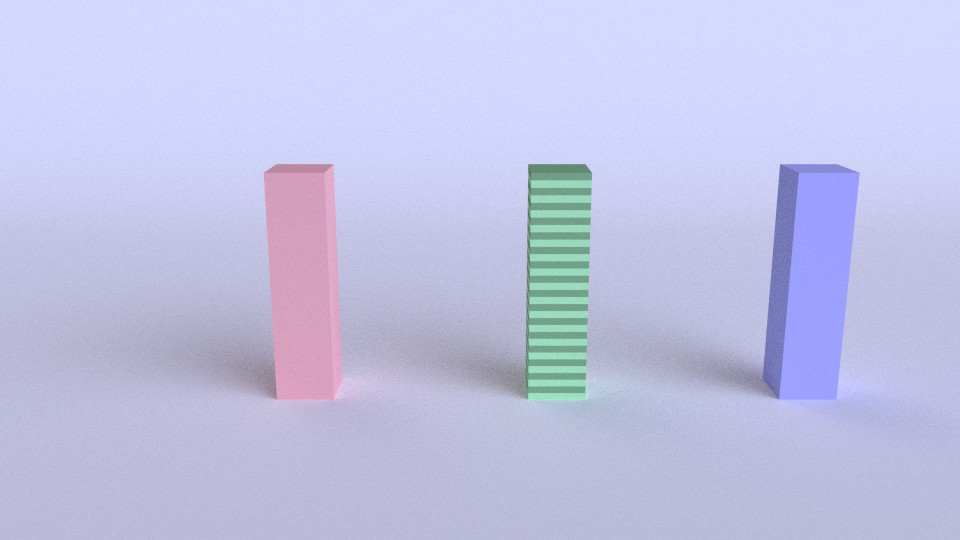
\includegraphics[width=0.47\columnwidth, trim=170px 105px 40px 105px, clip=true]{images/bend_l1_begin}
	}
	%\vrule
	\subcaptionbox{}{
		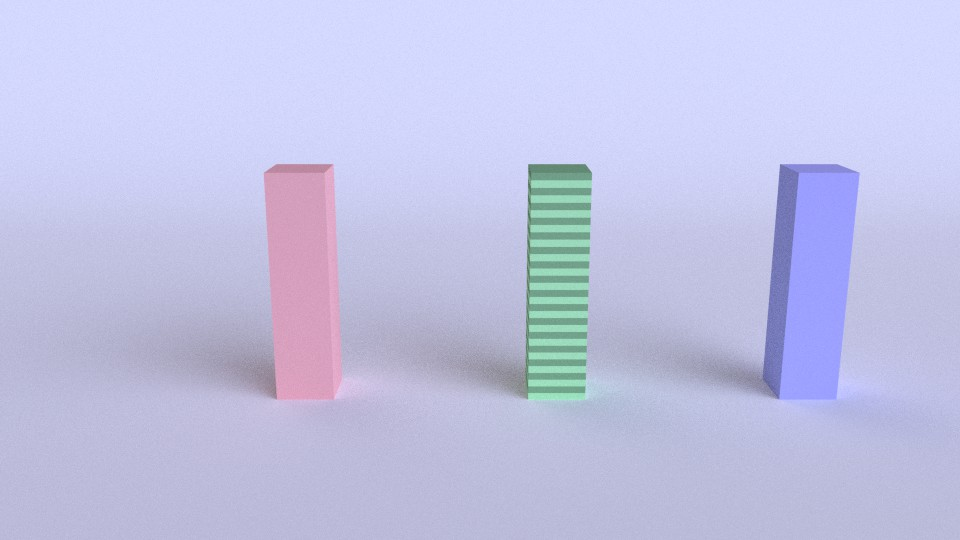
\includegraphics[width=0.47\columnwidth, trim=170px 105px 40px 105px, clip=true]{images/bend_l2_begin}
	}\\
	\subcaptionbox{}{
		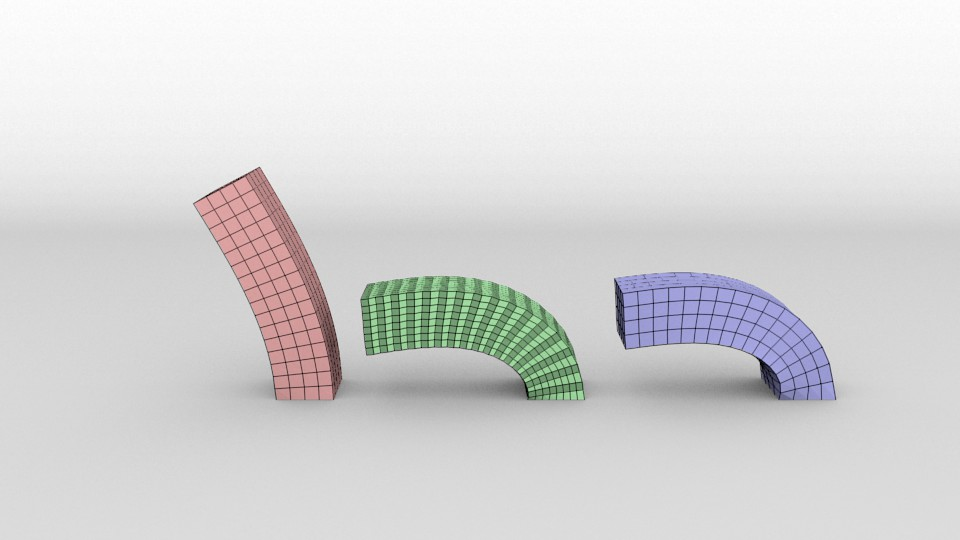
\includegraphics[width=0.47\columnwidth, trim=170px 105px 40px 105px, clip=true]{images/bend_l1_wire_end}
	}
	%\vrule
	\subcaptionbox{}{
		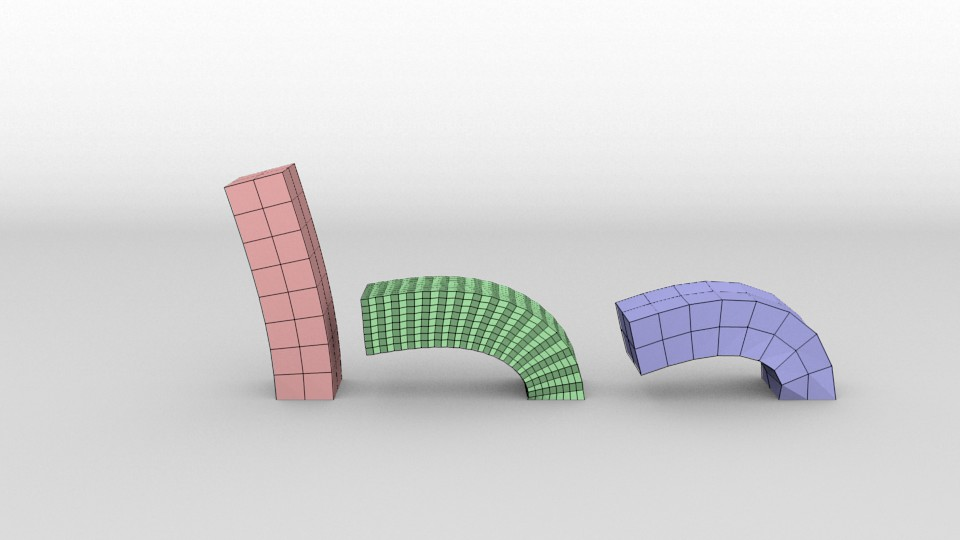
\includegraphics[width=0.47\columnwidth, trim=170px 105px 40px 105px, clip=true]{images/bend_l2_wire_end}
	}
	%\vspace{-8pt}
	\caption{Bending a heterogeneous bar: We compare {\DDFEM} to {\Naive} and a {\HiRes}. Subfigures (a, c) show comparison for 
		1 level of coarsening, and (b, d) show 2 levels of
		coarsening. The na\"{i}ve coarsening
		approach results in a much stiffer behavior, whereas our fitted
		model more closely approximates the fine model.}
	\label{fig:bending}
\end{figure}
\begin{figure}[t]
	\centering
	\begin{tabularx}{0.92\columnwidth}{ Y Y }
		\textbf{1 Level of Coarsening} & \textbf{\textbf{2 Levels of Coarsening}} \\
		\textbf{50x Faster} & \textbf{332x Faster}
	\end{tabularx}\\
	\subcaptionbox{}{
		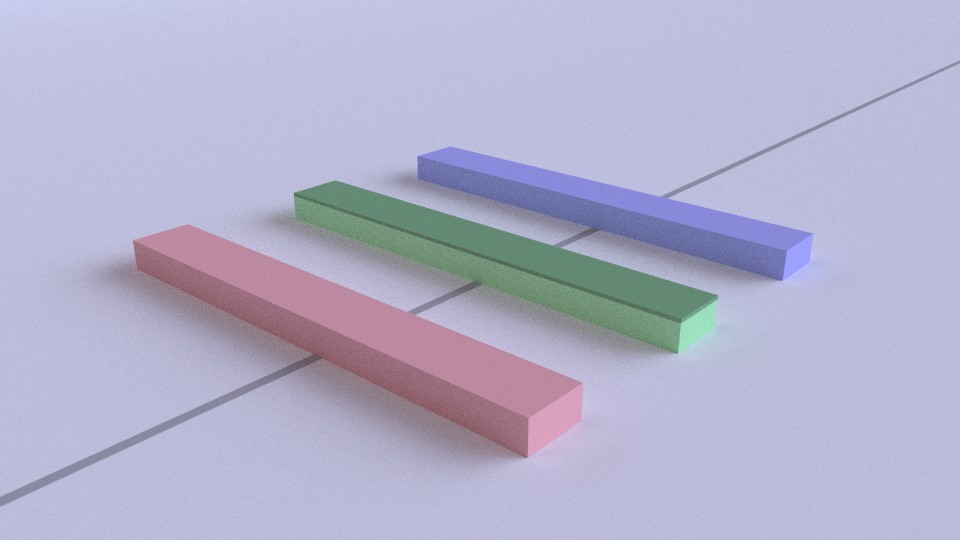
\includegraphics[width=0.47\columnwidth, trim=105px 60px 70px 115px, clip=true]{images/buckle_l1_begin}
	}%\vrule
	\subcaptionbox{}{
		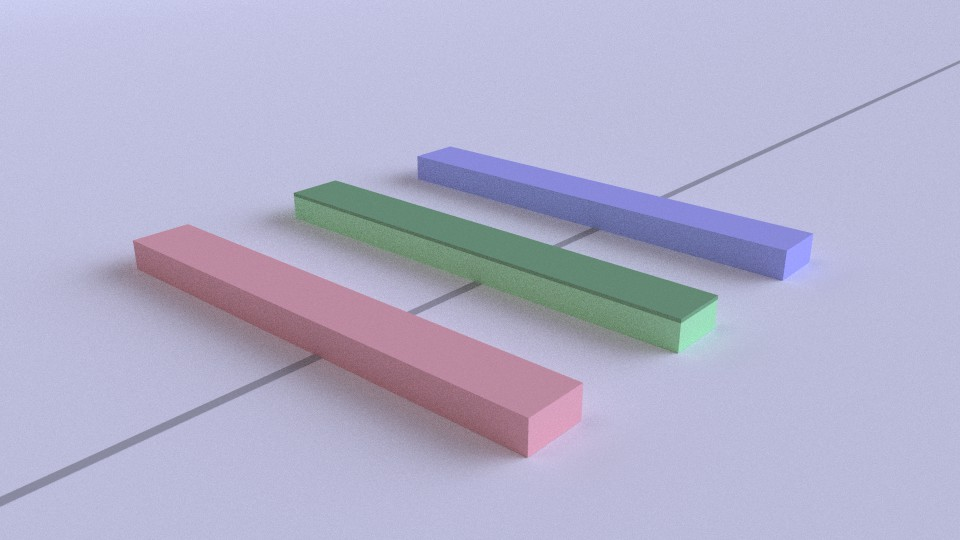
\includegraphics[width=0.47\columnwidth, trim=105px 60px 70px 115px, clip=true]{images/buckle_l2_begin}
	}
	\\
	\subcaptionbox{}{
		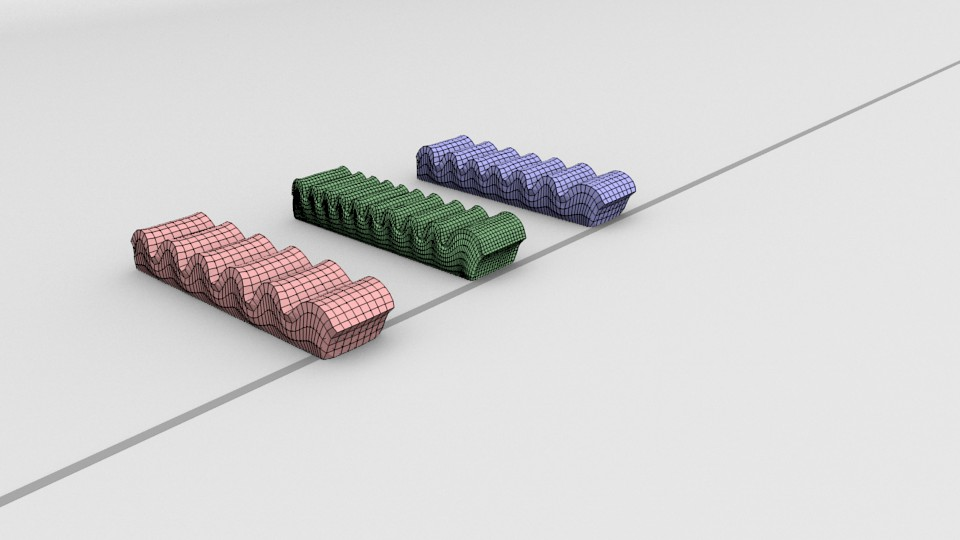
\includegraphics[width=0.47\columnwidth, trim=105px 60px 70px 115px, clip=true]{images/buckle_l1_wire_end}
	}
	%\vrule
	\subcaptionbox{}{
		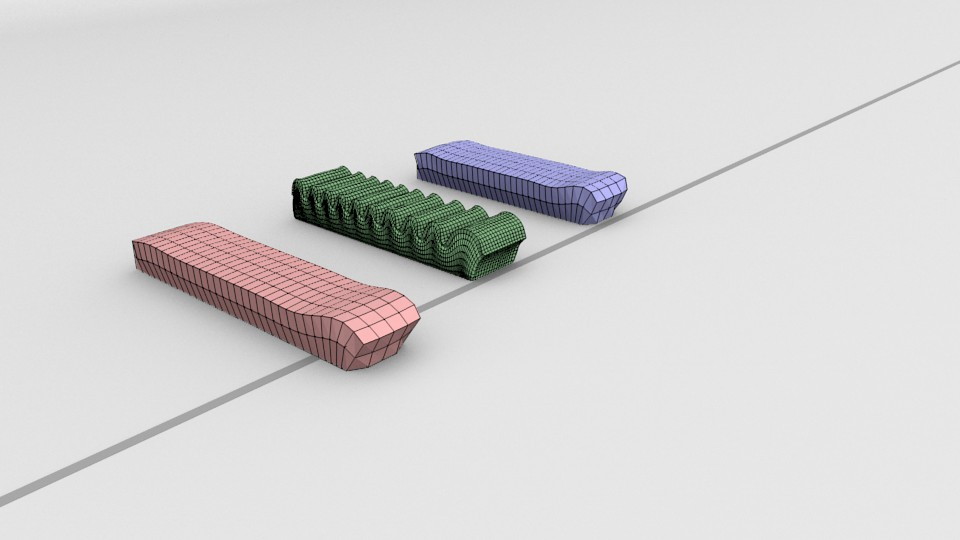
\includegraphics[width=0.47\columnwidth, trim=105px 60px 70px 115px, clip=true]{images/buckle_l2_wire_end}
	}
	\vspace{-2pt}
	\caption{Compressing a heterogeneous slab using {\Naive} (1 level and 2 levels of coarsening), {\DDFEM} (1 level and 2 levels of coarsening) and a {\HiRes}. The top, darker layer is stiffer, causing the object to buckle. The bottom vertices are constrained to stay on the floor. Figure (a,b) shows the slabs before compression, figure (c,d) shows the slabs after compression and figure. Notice that, after 1 level of coarsening, {\Naive} neither compresses nor buckles as much as either {\DDFEM} or {\HiRes}. After 2 levels of coarsening, \note{the buckling behavior is lost.}
		The {\Naive} fails to capture the compressive behavior of {\HiRes}, whereas {\DDFEM} does.}
	\label{fig:buckling}
\end{figure}
\begin{figure}
	\centering
	\begin{tabularx}{0.92\columnwidth}{ Y Y }
		\textbf{1 Level of Coarsening} & \textbf{\textbf{2 Levels of Coarsening}} \\
		\textbf{51x Faster} & \textbf{489x Faster}
	\end{tabularx}\\
	\subcaptionbox{}{
		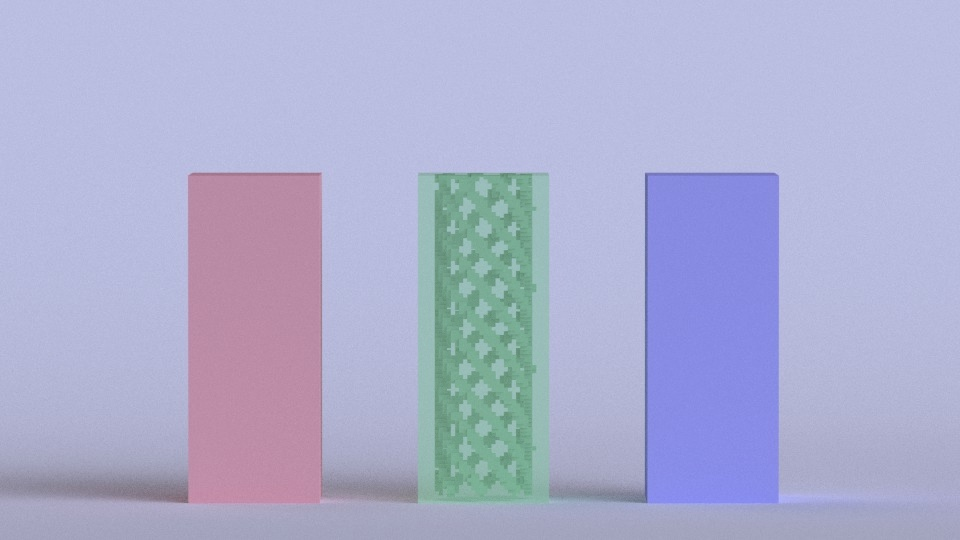
\includegraphics[width=0.4\textwidth]{images/fiber_l1_xray_begin}
	}%\vrule
	\subcaptionbox{}{
		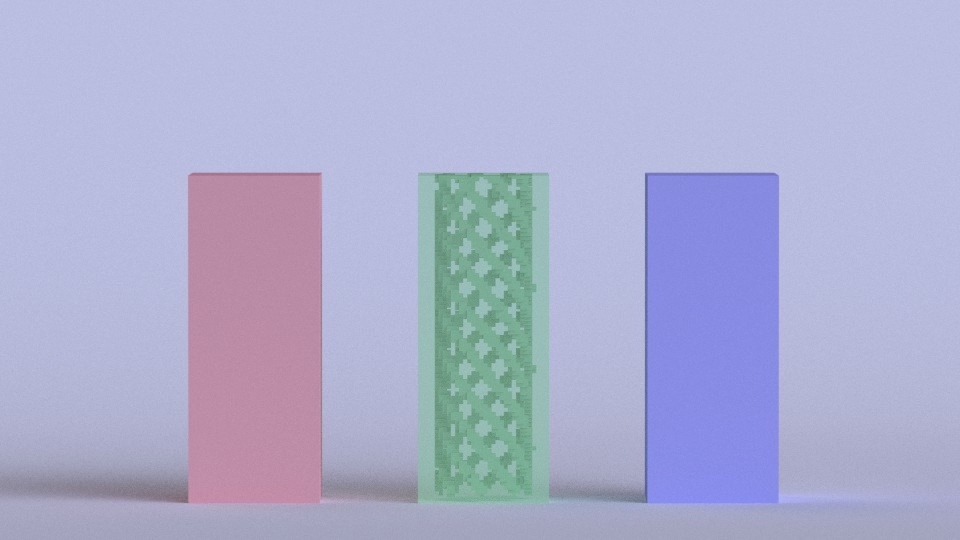
\includegraphics[width=0.4\textwidth]{images/fiber_l2_xray_begin}
	}  \\

	\subcaptionbox{}{
		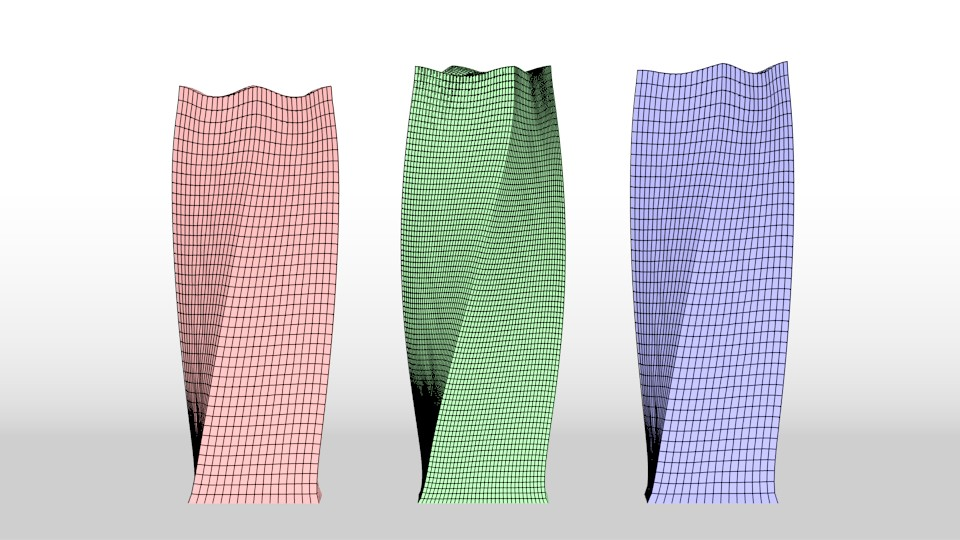
\includegraphics[width=0.4\textwidth]{images/fiber_l1_wire_end}
	}%\vrule
	\subcaptionbox{}{
		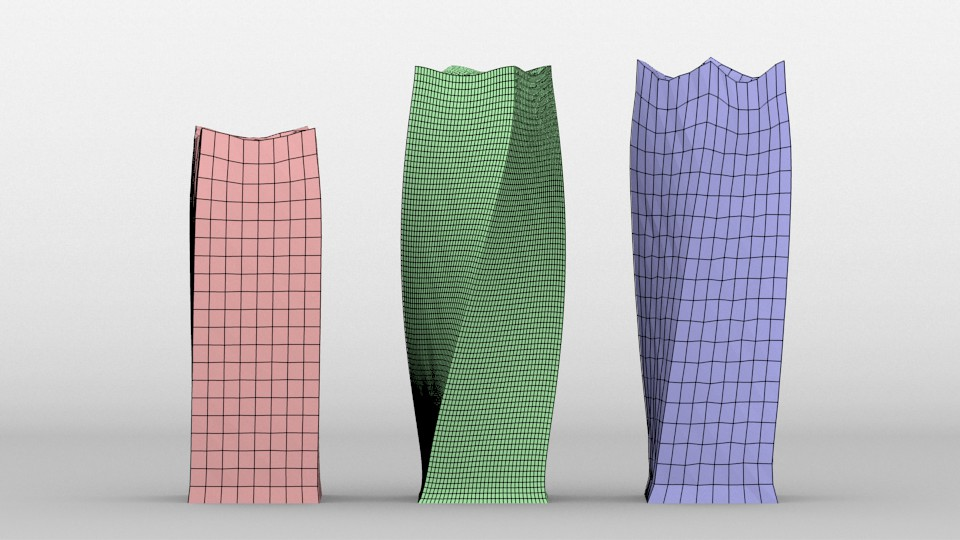
\includegraphics[width=0.4\textwidth]{images/fiber_l2_wire_end}
	}
	\vspace{-2pt}
	\caption{Simulating a bar with an embedded set of fibers using {\Naive}, {\DDFEM} and a {\HiRes}. Note that {\DDFEM} captures the characteristic twisting motion of the bar better than {\Naive}.  (a,b) shows the initial state of both bars while (c,d) shows the deformed state after pulling on the top of the bars.}
	\label{fig:fiberPull}
\end{figure}
\section{Results and Discussion}
\label{sec:result}
All the results shown here are simulated using nonlinear constitutive models at the fine scale. This and coarsening speed are the key differentiating factors between DDFEM and other coarsening algorithms such as~\citet{Nesme2009} and~\citet{Kharevych2009}.
\note{Our database starts with three Neo-hookean base materials with Young's modulus $1e5, 1e6, 1e7$ and Poisson's ration $0.45$. For comparison with 3D-printed objects, we used two base materials with measured Young's moduli.
	We use $500$ force directions, and sample $5$ magnitudes in each direction,
	resulting in $2500$ force samples for each material combination.
	In addition, we generate $500$ stretching samples for computing the direction of anisotropy. During fitting, we use shear modulus and Lam\'{e}'s first parameter,
	as well as the spring stiffness.
	We repeat the same process for the second level of coarsening, using
	$6561$ materials in the first level as base materials. We select
	$400$ representatives at each intermediate level.}

\subsection{Database}
One advantage of our compact coarse material representation is the small amount of storage it requires. In fact we require only $6\times8=48$ floating-point values for each material at the first coarsening level and $6\times64=384$ values for the second level.
(For each finer element, $^0\vr{p}$ contains 2 material moduli plus $C, \vr{v}$.)
For further recursive levels, we can limit ourselves to $320$ values per material.
Our current 3 material database is $4$ megabytes in size.

\subsection{Simulation Results}
We show results from elastostatic simulations performed using DDFEM. We also demonstrate its performance advantages over high-resolution simulations. We render wire frames to show the discretizations of the high-resolution and coarse meshes. We first show examples of two simple simulations, the pushing and twisting of a rectangular object with heterogeneous, layered material distribution (\autoref{fig:accuracy}). Note that in all cases DDFEM qualitatively matches the behavior of the high-resolution simulation. We also compare the performance of DDFEM to a na\"{i}ve coarsening method that uses the material properties from 2$\times$2$\times$2 element blocks of the high-resolution simulation mesh at each corresponding quadrature point. \note{In our supplemental video we compare to a second baseline model which averages material parameters inside each coarse element. This average model is less accurate than the Na\"{i}ve model in all cases.} 

Na\"{i}ve approaches often exhibit pathological stiffness  for heterogeneous materials (illustrated by the lack of compression of the box and lack of twisting of the bar)~\cite{Nesme2009}. In these cases, DDFEM yields good speed ups while maintaining accuracy. For a single level of coarsening we achieve \emph{8 times or greater} speed ups for all examples. Performance numbers and mean errors are listed in \autoref{table:performance}.
Since the fine simulation and the coarse simulation have different numbers of vertices, we create a fine mesh from the coarse simulation by
trilinearly interpolating the fine vertices using the coarse displacements. The errors are measured by computing the average vertex distance relative
to the longest dimension of the bounding box in rest shape.
We also examine the behavior of DDFEM during bending (\autoref{fig:bending}). Yet again the na\"{i}ve coarsening method completely fails to capture the behavior of the high-resolution result, while DDFEM offers a much better approximation. 
\paragraph{Performance Analysis}
\note{\autoref{table:quadPerformance} shows time spent in quadrature evaluation versus in solver at coarse and fine levels.
	We use $8$ quadrature points for the first level of coarsening 
	and $64$ for the second level. The time for computing the local stiffness matrix for one element increases from $0.1$ms to $1$ms.
	In the second level, the speedup comes from the reduced number of elements over which to perform quadrature and the time required for the linear solver.
	
	To further investigate the performance of our coarsened simulations
	we replaced Pardiso with an assembly-free
	Jacobi-preconditioned conjugate gradient (CG) linear solver and used this to simulate our George-bone test case.
	While the overall runtime of the high-resolution simulation increased from $496$ to $2082$ seconds (most likely do to the unoptimized nature of our solver) our coarsened model achieved 20x and 67x speedups using one level and two levels of coarsening respectively. 
	One might expect no benefit from the second level of coarsening since the 
	number of quadrature points remains constant. 
	However, the number of CG iterations is roughly proportional to the number of vertices in the simulation mesh and thus the coarse model converges more quickly~(\autoref{fig:cg}).
	Since our coarse material models are not restricted to use
	a fixed number of quadrature points,
	one could design coarse models that are more tailored towards
	assembly-free solvers by reducing the number of quadrature points and simplifying the strain energy expressions.
}

\begin{figure}
	\centering
	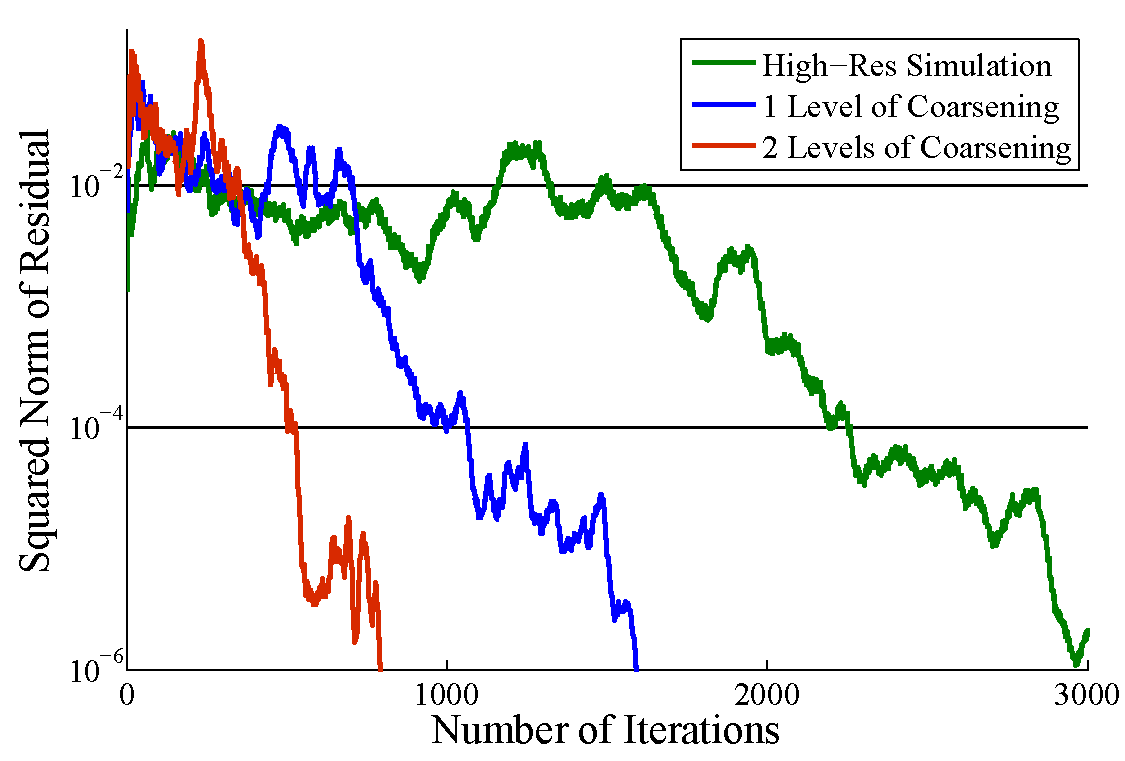
\includegraphics[width=0.6\textwidth]{figs/CGConverge.pdf}
	\caption{
		\note{Comparison of CG iterations on high-resolution and coarsened meshes of the George-bone example.
			The squared residual is measured as $\|\mathbf{K}\mathbf{x}-\mathbf{f}\|^2$.
			We observe that CG converges much faster on coarse meshes.
		}
	}\label{fig:cg}
\end{figure}

\begin{table}
	\centering
	\footnotesize
	\begin{tabular}{l c p{1cm} p{1cm} r }
		\hline 
		\textbf{Example} &\textbf{grid size}&\textbf{quad/iter} (12)&\textbf{time/iter} (2-21)&\textbf{iters}\\
		\hline 
		{\color{HiResColor}Bending(0)} &8$\times$32$\times$8   &  0.11  &0.27 &28\\
		{\color{DDFEMColor}Bending(1)} &4$\times$16$\times$4   &  0.015 &0.028&22\\
		{\color{DDFEMColor}Bending(2)} &2$\times$8$\times$2    &  0.014 &0.015&22\\
		\hline
		{\color{HiResColor}Buckling(0)} &128$\times$8$\times$16&  1.0   &8.8 &32\\
		{\color{DDFEMColor}Buckling(1)} &64$\times$4$\times$8  &  0.11  &0.28&20\\
		{\color{DDFEMColor}Buckling(2) }&32$\times$2$\times$4  &  0.10  &0.12&7\\
		\hline
		{\color{HiResColor}Fibers(0)} &32$\times$100$\times$32 & 10.0   &193&17\\
		{\color{DDFEMColor}Fibers(1)} &16$\times$50$\times$16  &  1.0   &4.9&13\\
		{\color{DDFEMColor}Fibers(2)} &8$\times$25$\times$8    &  0.68  &0.96&7\\
		\hline
	\end{tabular}
	\caption{\note{Portion of time in seconds used by quadrature computation during static simulation in seconds. Bracketed numbers indicate corresponding lines in Algorithm \ref{alg:sim}.}}
	\label{table:quadPerformance}
\end{table}
\paragraph{Complex material behavior} DDFEM can capture the gross behavior of  complex, spatially-varying material distributions. \autoref{fig:buckling} shows the results of applying DDFEM to a non-linearly elastic slab with a stiff ``skin.'' The bottom of the slab is constrained to slide along the ground with one end fixed. When force is applied to the free end of the slab, buckling occurs.  Somewhat obviously, DDFEM cannot replicate the frequency of the high-resolution buckling pattern due to the coarseness of the simulation mesh. However, it correctly captures the gross behavior of the bar and approximates the overall amount of compression well. \autoref{fig:buckling} also shows a comparison with 2nd level coarsening. In this case, the overall compression of the bar is still captured accurately. For this example DDFEM affords \emph{50 times} (1 level of coarsening) and \emph{332 times}  (2 levels of coarsening) performance improvements over the high-resolution simulation.  The artificial stiffness of the na\"{i}ve model can be seen in the reduced buckling and compression when compared to DDFEM at both coarsening levels.
%\vspace{-8pt}
\paragraph{Anisotropic material distribution} Next we explore the ability of DDFEM to handle highly anisotropic material distributions (\autoref{fig:fiberPull}). Specifically, we embed a helical set of stiff fibers in a soft, non-linearly elastic matrix. Pulling on the object induces a twisting. Again, at one coarsening level DDFEM captures this anisotropic behavior well, much better than the naive approach, and gains a \emph{51 times} speed up over the high-resolution simulation. Worth noting is that the DDFEM bar is slightly softer in the $y$-direction. This kind of inaccuracy should be expected. Since our method builds a low-dimensional approximation of a potential energy function we cannot hope to accurately reproduce the complete behavior of the high-resolution simulation.  What is important is that DDFEM captures the salient global behavior, in this case, the twisting of the bar. 
\paragraph{Geometry and material design} We present three examples of using DDFEM for geometry and material design. In the first example, we edit the material composition of the sole of a running shoe in order to stabilize it. \autoref{fig:shoe} shows the effect of the three material edits as well as relative speed up achieved over the full resolution simulation and coarsening time. DDFEM performance is always an order of magnitude more than that of the high-resolution simulation, and, most importantly, our coarsening times are on the order of milliseconds. We stress that our current implementation is completely single threaded and that coarsening, which in our case involves a simple database lookup, is inherently parallel.
In the second example, we add a supporting arch to a bridge. Prior to the addition of the support structure, the bridge sags catastrophically. The fast coarsening of DDFEM allows us to achieve an 8 fold increase in simulation performance using a single coarsening pass. In the third example, we add a rigid skeleton to a deformable character (George) in order  to control his pose. Here our single threaded, data-driven coarsening only takes ~200ms.  
\begin{figure}
	\centering
	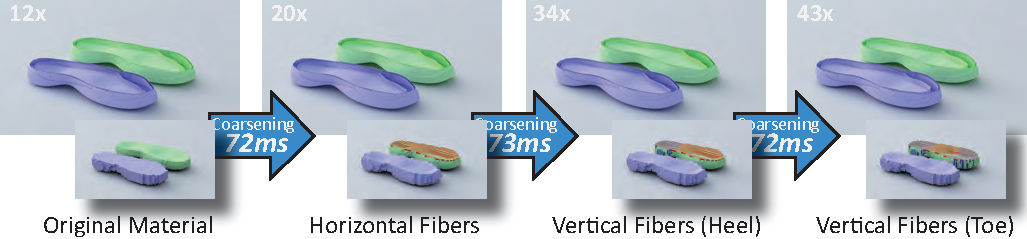
\includegraphics[width=0.90\textwidth]{images/DesignExampleShoe}
	\caption{Designing a shoe sole: We compare the performance of {\DDFEM} to that of {\HiRes} in the context of a material design problems. Large images show the effect of material changes on the sole of the shoe, which is being deformed under a ``foot-like'' pressure field. Inset images show the materials assigned to the shoe sole and the embedded finite element simulation mesh. Numbers within arrows show coarsening times between editing steps and the numbers in the upper left corner of each image show the relative performance of {\DDFEM} to  {\HiRes}. While the {\DDFEM} sole is made up of many coarse material, we display it as a single color to distinguish it from the {\HiRes}.}
	\label{fig:shoe}
\end{figure}

\begin{figure}
	\centering
	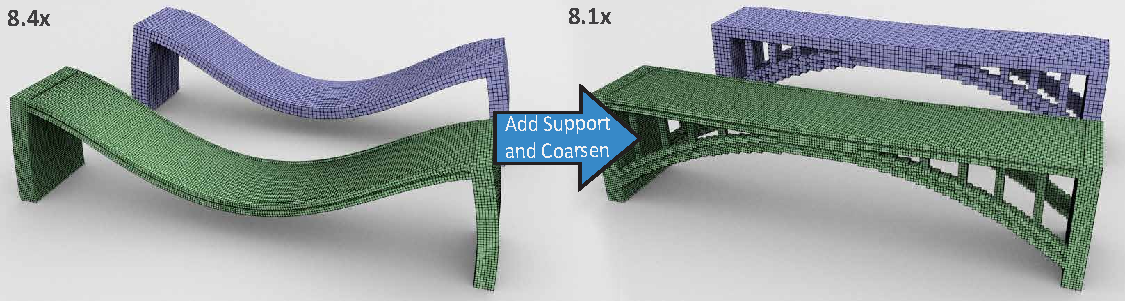
\includegraphics[width=0.8\textwidth]{images/bridge.pdf}
	\caption{Accelerating geometry change: We repair a structurally unsound bridge by adding a supporting arch (8x faster).}
	\label{fig:bridge}
\end{figure}
\begin{figure}
	\centering
	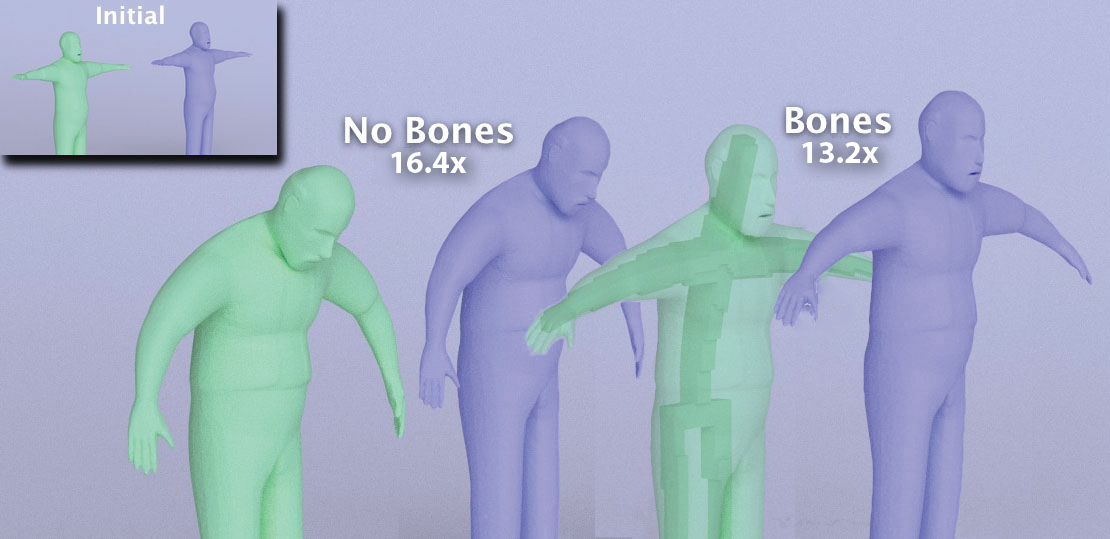
\includegraphics[width=0.8\textwidth]{images/georgeUpdate.png}
	\caption{Correcting George's posture using a rigid skeleton ({\HiRes} and {\DDFEM}).}
	\label{fig:george}
\end{figure}
\paragraph{Dynamics} Though the examples shown in this paper focus on static analysis, DDFEM is equally applicable to dynamic simulations. At its core, DDFEM simply supplies new, more accurate material models for use during simulation. This makes the method useful for accelerating various animation tasks as well. In the accompanying videos we show a dynamic simulation of our fiber embedded bar, computed using a standard linearly-implicit time integrator.

\begin{figure}
	\centering
	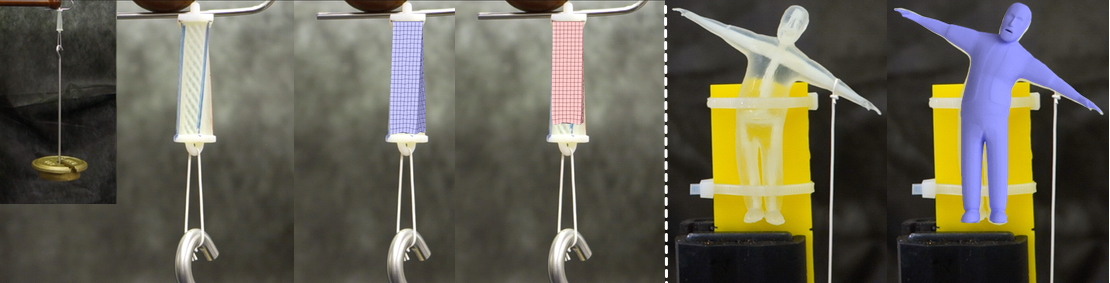
\includegraphics[width=0.8\textwidth]{images/experiments.jpg}
	\caption{A comparison of  {\DDFEM} (2 levels of coarsening) to real world deformations of 3D printed, multi-material designs. {\DDFEM} captures the twisting behavior of an anisotropic bar much more accurately than {\Naive}. Similarly {\DDFEM} accurately predicts the deformation of our heterogeneous George character. }
	\label{fig:experiments}
\end{figure}

\subsection{Fabricated Results}
Finally, we test the accuracy of our simulation against fabricated results, created using a Stratysys Object Connex 500 multimaterial 3D printer. We fabricated a bar with embedded helical fibers as well as our George character and applied specified loads to both. We show qualitative comparison of the deformed configurations of these real-world examples to our simulated results (\emph{2 levels of coarsening}-\autoref{fig:experiments}). Note that the simulation does an excellent job of predicting the deformed configuration of both objects.

\section{Limitations and Future Work}
Because DDFEM relies on a database compression step to combat the combinatorial explosion of coarse materials,  accuracy is heavily influenced by the set of representative coarse materials. Finding a better way to select coarse structures is an interesting area of future work.
Second, in our attempt to make our method geometry independent, some accuracy when dealing with partially filled boundary finite elements is sacrificed. Adding a parameterized boundary representation to the method, in order to more correctly handle non-axis aligned boundary conditions, could also be explored. Third, the method acts on discrete materials. While we believe that this is reasonable, considering the way that engineers and designers approach material design, a method that coarsens continuous spaces of non-linear materials could be beneficial.   

Many avenues of future work are promising. First, one could explore topologically aware meshing (i.e. in the same vein as~\citet{Nesme2009}) to allow better handling of models with large empty regions.
In fact shape function learning approaches, such as~\citet{Nesme2009} could be combined with our material learning approach to produce even more accurate simulations. Including these shape functions in our database could, for instance,  allow us to capture the wrinkles in our buckling example. Second, extending DDFEM to more complex material models, such as those involving plasticity, would be a useful exercise.
Third, DDFEM can be combined with an adaptive voxel grid as well as other dynamic meshing approaches to obtain further speed-ups.  Finally,  exploring hierarchical solvers based on DDFEM coarsening is a very attractive direction. Solvers such as multigrid methods rely on good coarse approximations to accelerate fine scale simulations. Using DDFEM for these approximations could improve the convergence rate, and thus the performance of such algorithms. 

\chapter{Computational Design with Microstructures}
\label{ch3:topopt}
Many engineering problems are formulated as high level objectives such as the ability to support certain weight, optimal tradeoffs between compliance and mass, minimal deformation under temperature changes, etc. A popular approach to design such structures is topology optimization.
Topology optimization generally refers to discretizing the object of interest into small elements and optimizing the material distribution over these elements such that the functional goals are satisfied \cite{bendsoe2004topology}.
Traditionally, topology optimization focuses on designs made of homogeneous materials and is concerned with macroscopic changes in the object geometry.
With the advent of multi-material 3D printing techniques, it is now possible to assign materials at a much higher resolution, allowing much finer designs and improved functional performances.
Unfortunately, standard techniques for topology optimization do not scale well and they cannot be run on objects with billions of voxels.
This is because the number of variables to optimize increases linearly with the number of cells in the object.
Since many current 3D printers have a resolution of 600DPI or more, a one billion voxel design occupies only a 1.67 inch cube.

Most previous algorithms use a single material property variable such as density or material stiffness in each cell,
for which analytical formulas describing the property bounds exist \cite{Allaire93Bounds}.
On the contrary, optimizing the structure and material distribution of an object in a high dimensional material property space remains an open problem.
In this work, we propose a new computational framework for topology optimization with microstructures that supports design spaces of multiple dimensions.
We start by computing the gamut of the material properties of the microstructures by alternating stochastic sampling and continuous optimization.
This gives us a {\it discrete} representation of the set of achievable material properties, 
from which we can construct a {\it continuous} gamut representation using a level set.
We then reformulate the topology optimization problem in the continuous space of material properties and propose an efficient optimization scheme that finds the optimized distributions of multiple material properties simultaneously inside the gamut.
Finally, in order to obtain fabricable designs, we map the optimal material properties back to discrete microstructures from our database.

Our general formulation can be applied to a large variety of problems. We demonstrate its efficacy by designing and optimizing objects in different material spaces using isotropic, cubic and orthotropic materials. We apply our algorithm to a diverse range of functional objectives such as minimal compliance and target strain distribution. 
Furthermore, our approach utilizes the high-resolution of current 3D printers by supporting designs with one trillion voxels.
We fabricate several of our designs to demonstrate practical applications of our method in 3D printing.
The main contributions of our work can be summarized as follows:
\begin{itemize}
	\item We present a fully automatic method for computing the space of material properties achievable by microstructures made of a given set of base materials.
	\item We propose a generic and efficient topology optimization algorithm capable of handling objects with a trillion voxels. The key of our approach is a reformulation of topology optimization to work directly on continuous variables representing the material properties of microstructures. This allows us to greatly reduce the problem scale for it to be efficiently solved with state of the art solvers.
	\item We validate our method on a set of test cases and demonstrate its versatility by applying it to various design problems of practical interest.
\end{itemize}
\section{Overview}
Given as input a set of base materials, an object layout, and functional objectives, the goal of our system is to compute the material distribution inside the object in order to optimize these functional objectives. In our approach, we do not solve the problem directly, instead we work with microstructures made of the base materials. The complete pipeline of our system has three stages (Figure \ref{fig:overview}).
\begin{figure}
	\centering
	\includegraphics[width=.95\linewidth]{figs/Overview.pdf}
	\caption{
		Algorithm overview. We start by precomputing the gamut of material properties that can be achieved with all material microstructures of a given size. Next, we run our topology optimization algorithm that optimizes the material properties of the object within this gamut such as to minimize some functional objective. Finally, we map the optimal continuous material properties back to microstructures from our database to generate a printable object.
	}
	\label{fig:overview}
\end{figure}
\paragraph{Material Space Precomputation}
In the first stage, we estimate the gamut of material properties covered by all possible microstructures made by spatial arrangement of base materials. 
Since exhaustively computing the properties of all these microstructures is, in practice, intractable, we progressively increase the material space by alternating a stochastic search and a continuous optimization. The first step introduces discrete changes in the materials of the microstructures and allows emergence of new types of microstructures. The second step allows to locally push the material space boundaries by refining the microstructure shapes. After completing this stage, we obtain a discrete representation of the space of material properties and the mapping between these properties and the corresponding microstructures.

\paragraph{Gamut-based Continuous Topology Optimization}
In the second stage, we construct a smooth continuous gamut representation of the material property space by using a level set field. We define our topology optimization problem directly in this space. Our approach minimizes the objective function over possible material parameters while asking for strict satisfaction of the physics constraints -- typically, the static equilibrium -- as well as the strict satisfaction of the physical parameter bounds. Taking advantage of our gamut representation as a level set, we formulate this last constraint as limiting the material properties to stay on the negative side of the level set. This guarantees that the material properties that we use in the optimization are always physically realizable.

\paragraph{Fabrication-oriented Microstructure Mapping}
In the last stage, we generate a printable result by replacing each cell in the object layout with a microstructure whose material properties are the closest to the continuous material assignment resulting from the optimization. We also take into account the boundary similarity across adjacent cell interfaces to improve the connectivity between microstructures. This results in a high-resolution, multi-material model with optimized functional specifications.

\section{Material Space Exploration}
\label{sec:sampling}
\begin{figure}
	\centering
	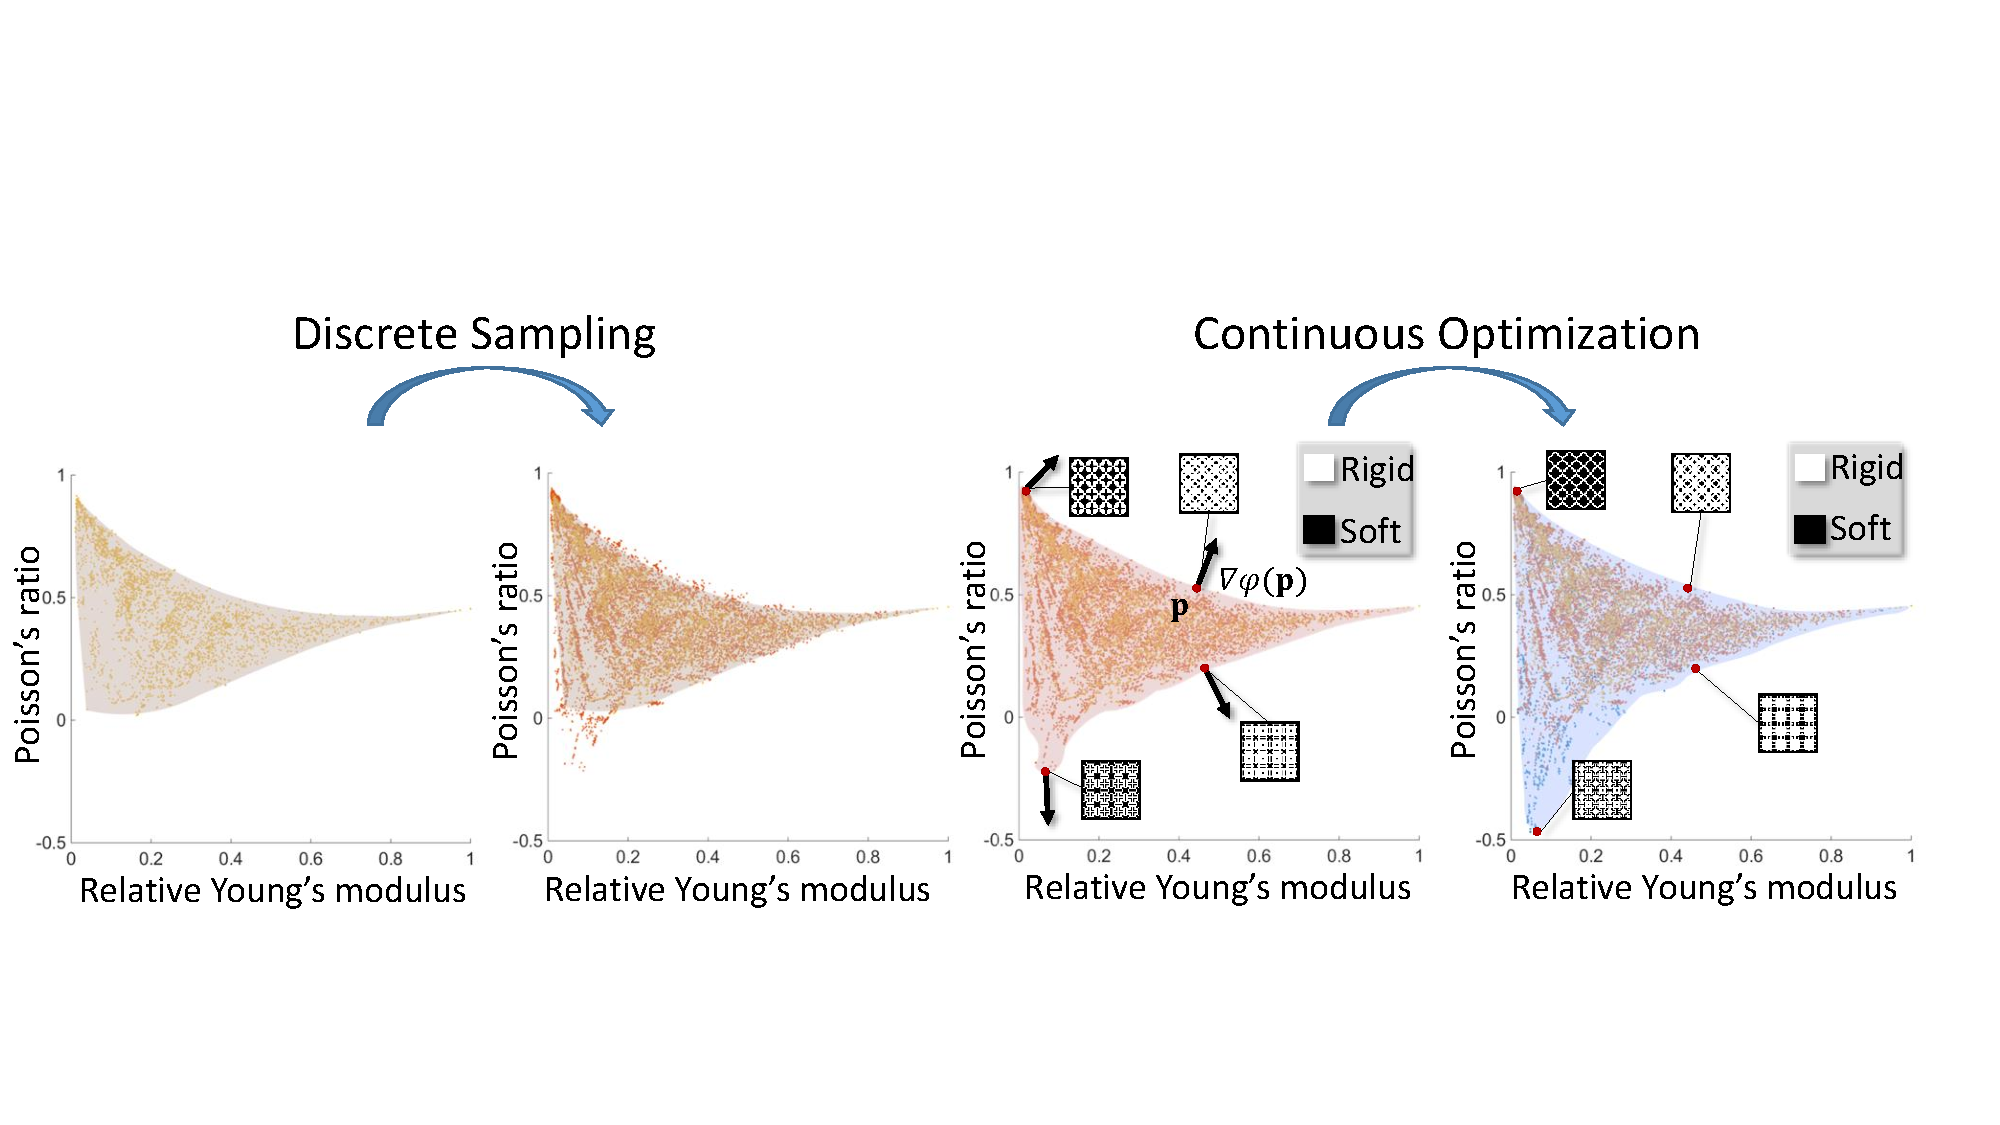
\includegraphics[width=.95\linewidth]{figs/topsampling.pdf}
	\caption{One cycle of computing the microstructure gamut. 
		Given a set of samples, we compute a signed distance function approximating the material gamut (\emph{left}) and randomly perturb microstructures lying near the boundary to provide new seeds to the continuous algorithm (\emph{middle left}). We then update the distance field and use the gradient of the signed distance function at the the boundary to define new target material points (\emph{middle right}). These target material points are used in a continuous optimization that generates new samples (\emph{right}).} 
	\label{fig:lssampling}
\end{figure}

The first step in our pipeline is to determine the range of achievable physical properties when combining the base materials into microstructures at a given resolution.
Computing the mechanical properties of microstructures arranged in periodic tilings can be performed using physics-based simulation.
We use the homogenization theory to compute the elastic properties of each microstructure~\cite{Allaire2012,Schumacher:2015,Panetta:2015}.
However, while inferring the homogenized properties of individual microstructures is not particularly challenging, analyzing the space covered by {\it all} combinations of base materials is much more difficult due to the combinatorial explosion in the number of possible material arrangements.
As an example, $16\times16\times16$ lattices made of only two materials corresponds to $2^{4096}$ microstructures.
Exhaustively simulating all microstructures is clearly infeasible in practice.
To address this issue, two possible avenues can be pursued:(i) sample the space of microstructures, (ii) take advantage of the continuity between material parameters of the individual voxels and macroscopic properties of the microstructures in order to generate new microstructures with desired properties.
The second option is effective in reaching locally optimal values in the material property space.
However, the continuous function that maps the material assignment to material properties is nonlinear.
In particular, very different microstructures can correspond to the same point in the material property space.
Additionally, since the ratio of materials in each cell is bounded between zero and one, the continuous optimization converges slowly or stops moving when material distributions in many cells are at the lower or upper bound.
Being able to jump out of a local optimum and discovering different variants is important in order to provide new exploration regions.
We combine the strength of these two approaches in a scheme that alternates between a stochastic search and a continuous optimization. We provide the technical details in the rest of this section.

\subsection{Discrete Sampling of Microstructures}
We aim at sampling the space of material assignments, i.e. microstructures, in a way that maximizes the number of samples whose material properties lie in the vicinity of the material gamut boundaries.
We do not draw all samples at once but progressively enrich the database of microstructures as we refine our estimation of the material gamut boundaries.
This sampling strategy is motivated by the observation that a small change in the material assignment of a microstructure generally -- but not always -- translates to a small change of its material properties.
By modifying microstructures located near the current boundaries of the material property gamut, we are likely to generate more structures in this area, some of which will lie outside of the current gamut.

Given a population of microstructures to evolve, we generate new samples from each microstructure by changing adding or subtracting random beams.
To rationalize computational resources, we want to avoid revisiting the same voxel twice. But we do not want to privilege any particular order either.
\citet{Ritchie2015SOCM} recently presented a Stochastically-Ordered Sequential Monte Carlo (SOSMC) method that provides a suitable approach.
In SOSMC, a population of particles (microstructures) corresponding to instances of a procedural program (the assignment of materials to the voxels of the microstructures)
are evolved so as to represent a desired distribution.
During this process, the programs are executed in a random order and particles are regularly scored and reallocated in regions of high probability.
In our particular settings, we use the scoring function
\begin{equation}
s(\mathbf{p_i}) = \frac{\Phi(\bf p_i)}{D(\bf p_i)} \times \frac{1}{D(\bf p_i)},
\label{eq:score_fct}
\end{equation}
where $\Phi(\bf p_i)$ is the signed distance of the material properties of particle $i$ to the gamut boundary (see Section \ref{sec:ls}) and $D(\bf p_i)$ is the local sampling density at the location $\bf p_i$. We define the sample density as
\begin{equation}
D(\bf p_i)=\sum_{k}\phi_{k}(\bf p_i)\ ,
\end{equation}
where $\phi_{k}(\bf p)=\left(1-\frac{||\bf p-\bf p_{k}||^{2}_{2}}{h^{2}}\right)^{4}$ are locally-supported kernel functions that vanish beyond their support radius $h$, set to a tenth of the size of the lattice used for the continuous representation of the material gamut (see Section \ref{sec:ls}).

The first term in Equation \ref{eq:score_fct} favors microstructures located near the gamut boundary. The normalization by $D$ allows us to be less sensitive to the local microstructures density and to hit any location corresponding to the same level-set value with a more uniform probability. The second product is used to additionally privilege under-sampled areas.

Particles are resampled using systematic resampling scheme \citep{Douc05resamplingSchmes} that is also used to initiate the population of particles. These particles are then evolved by adding and subtracting beams with random sizes. The sampled structures are then cleaned by removing unsupported components and filling enclosed cavities.

\subsection{Continuous Optimization of Microstructures}
The goal of the continuous optimization is to refine the geometry of the microstructures located at the boundary of the gamut in order to further expand the gamut along the normal directions (Figure \ref{fig:contMicro}).
\begin{figure}[h]
	\centering
	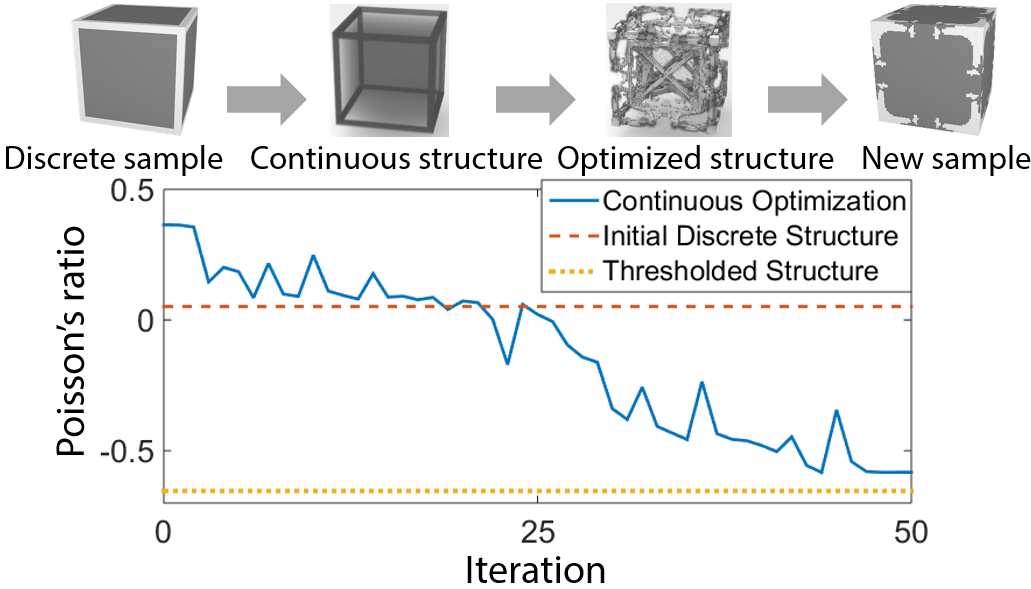
\includegraphics[width=0.9\textwidth]{images/contOpt.png}
	\vspace{-0.2cm}
	\caption{The continuous sampling step uses topology optimization to expand the gamuts by refining existing structures. A good starting point is necessary for the optimization to find better solutions. 
		We use discrete microstructures near the boundary to initialize topology optimization. 
		At convergence, we threshold the values to obtain a new discrete sample.}
	\label{fig:contMicro}
\end{figure}
We start continuous sampling by selecting a subset of microstructures lying on the boundary of the gamut.
The discrete structures are mapped to continuous values close to $0.5$.
We used $0.5\pm0.3$ in our experiments.
Doing so allows the topology optimization algorithms to move freely in the first steps and discover new structures.
We show an example of reducing the Poisson's ratio of an initial structure in Figure \ref{fig:contMicro}.
In the plot, the initial Poisson's ratio is close to $0.4$ since the starting point is similar to a homogeneous block.

For each starting structure, we identify target material parameters using the gradient of the level set $\Phi$ at the initial discrete sample point $\bf p$ (see Section \ref{sec:ls}) defined by ${\bf q} = {\bf p} + \nabla \Phi ({\bf p})$.
We translate this target material parameters into an elasticity tensor $\bC_0$ and density $\rho_0$. Here $\rho$ is the ratio of the two base materials in the microstructure.

Note that our problem formulation does not restrict us to a particular topology optimization algorithm or material distribution parametrization. We have experimented with two objective functions that worked equally well for our purposes.
The first objective uses an energy based formulation~\cite{xia:2015:design} to compute and optimize the elasticity tensor directly. At a high level, the optimization problem is
\begin{equation}
\arg\min_{\bx} f(\bx) = (\bC(\bx)-\bC_0)^2 + w_{\rho}(\rho-\rho_0)^2, \quad \rho = \sum_{i} x_{i} ,
\end{equation}
where $\bx$ is the ratio of materials in each cell, and $w_{\rho}$ controls the weighting between the displacement term and the density term.
The authors of the method developed parameter heuristics to optimize for difficult cases such as negative Poisson's ratio structures. We naturally arrive at structures with negative Poisson's ratio without the parameter varying step in~\cite{xia:2015:design} since our discrete samples allow us to explore a wide variety of initial designs.

The second objective is formulated using harmonic displacements~\citep{Kharevych2009,Schumacher:2015} $\bG$ instead of the elasticity tensor directly. $\bG$ is a $6\times 6$ symmetric matrix where each row corresponds to a strain in vector form. We use the target elasticity tensor $\bC_0$ to compute the target harmonic displacements matrix $\bG_0$ and minimize the objective function:
\begin{equation}
f(\bx) = (\bG(\bx)-\bG_0)^2 + w_{\rho}(\rho-\rho_0)^2.
\end{equation}
This objective matches soft structures more accurately since entries of $G$ are inversely proportional to material stiffness.

Following the work by \citet{andreassen2014design}, we use the method of moving asymptotes (MMA) \cite{svanberg1987method}) to optimize the objectives using an implementation provided in the NLOPT package \citep{johnson2014nlopt}. We run at most $50$ iterations since it usually converges to a solution within 20-30 steps (Figure~\ref{fig:contMicro}).
MMA makes large jumps during the optimization while keeping track of the current best solution, thus causing the oscillation of the objective value.
To force continuous material ratios towards discrete values, we experimented with the SIMP model with the exponent set to $3$ and the Hashin-Shtrikman bound for isotropic materials
described by~\citet{bendsoe1999material}.

Either interpolation allows us to threshold the final continuous distribution and obtain a similar discrete sample. We tolerate small deviations introduced by the thresholding since our goal is to obtain a microstructure lying outside of the gamut rather than reaching a particular target. In practice, we observed that the material properties of the final discrete structures often did not change significantly after the thresholding step. 

\subsection{Continuous Representation of the Material Gamut }\label{sec:ls}
We represent the gamut of material properties using a signed distance field that is computed from the material points associated to the sampled microstructures.
First, we normalize each coordinate $p_i$ of $\bf p$ to constrain the scope of the level set to an $n$-dimensional unit cube. Then we compute the level set values on the cell centers of an $n$-dimensional Cartesian grid that encloses this unit cube. We draw inspiration from the methods for surface reconstruction used in particle fluid rendering \cite{zhu2005animating,bhatacharya2011level,ando2013highly} and extend it to $n$ dimensions. In this case, a signed distance field is generated from a set of points by evaluating an implicit distance function $\Phi$ at each point $\mathbf{p}\in\mathcal{M}$.
We initialize the signed distance field using the implicit function $\Phi(\mathbf{p})=||\mathbf{p}-\bar{\mathbf{p}}||-r$ from~\citet{zhu2005animating} where $||\cdot||$ is the Euclidean distance between two points in $\mathcal{M}$, and $\bar{\mathbf{p}}$ is the average position of the neighboring points of $\mathbf{p}$ within a range of $2r$. Note that the signed distance is initially defined only near the boundary of the gamut. In order to sample the distance on the entire domain, we propagate the 0-level set surface using the fast marching algorithm and solve an explicit mean curvature flow problem defined as $\partial \Phi / \partial t = \Delta \Phi$~\citep{osher2006level} .

Having a continuous representation of the gamut of materials achievable by the microstructures, we can now reformulate the topology optimization problem directly in the material space.

\section{Discovery of Extremal Microstructure Families}
\label{sec:discovery}
Microstructures can exhibit remarkable physical properties that extend beyond the properties of their constituent materials.
Many microstructure types have been developed to demonstrate applications
in mechanics~\citep{milton1995,kadic2012practicability,meza2014strong,zheng2014ultralight,li2016mechanical,wang2016lightweight},
acoustics~\citep{fang2006ultrasonic,li2009experimental}, 
and electromagnetics~\citep{schurig2006metamaterial,shalaev2007optical}.
These microstructures are typically designed by domain experts using time and labor intensive manual processes. These designs are often programmable in the sense that they have a small number of parameters to generate a family of geometries. A given microstructure family can be tested by performing simulations or experimental measurements on a set of samples drawn from it. The mapping between parameters and physical properties discovered in this testing process helps uncover the underlying design principles that drive these correspondences.
In practical applications, mapping the parameter space also allows for the selection of a family member that has a desired tradeoff of physical properties~\citep{gibson1982mechanics}.
Unfortunately, it is rare for manually designed microstructure families to reach extremal properties. This is because the space of possible microstructure designs is combinatorial and therefore impossible to explore exhaustively.
One common approach to bypass this design challenge is to use computational methods,
such as topology optimization~\citep{sigmund1994materials,vogiatzis2017topology}, with a computer simulation in their inner loop to find a microstructure with a desired tradeoff of physical properties.
Unfortunately, constructing parametric models from these optimized structures has heretofore required further expertise and manual design effort~\citep{clausen2015topology}.
In contrast to previous work, we present the first computational method to automatically explore the space of microstructure designs and discover parametric families optimized for competing properties.

While our methodology is not limited to specific physical properties, this study applied our method to design of mechanical microstructures. Specifically, we set our algorithm to search for a particularly interesting type of mechanical microstructures: auxetic materials, which have a negative Poisson's ratio.
These materials have the unusual property of becoming laterally thinner under axial compression.
2D auxetic structures are well understood due to their relatively simple geometry such as reentrant structures~\citep{sigmund1994materials,lakes1987foam},
chiral structures~\citep{prall1997properties,ha2016chiral}
and rotating mechanisms~\citep{babaee20133d,buckmann2014three}.
Generalizing existing 2D structures to 3D is challenging since a naive arrangement of 2D mechanisms often results in orthotropic or other anisotropic structures with low shear resistance. Such structures will prefer shearing deformation when the load is not aligned well with the auxetic direction. Additionally, since Poisson's ratio for orthotropic structures is unbounded, orthotropic auxetic structures are much easier to find than isotropic ones18. Lakes fabricated and tested the first isotropic 3D auxetic structure13. However, designing manufacturable 3D auxetic structures remains a challenging task due to its complexity.
Only a handful of 3D design patterns have been fabricated and measured~\citep{andreassen2014design,saxena2016three}.
This study led to the discovery of five families with negative Poisson's ratio and tunable shear resistance.
\subsection{Discovery Pipeline}
\begin{figure}
	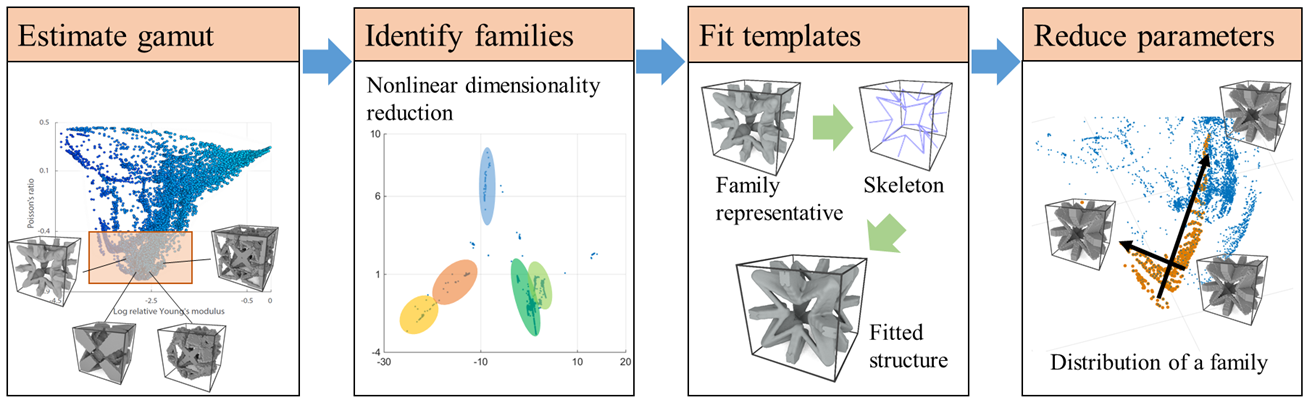
\includegraphics[width=\textwidth]{images/discoveryPipeline.png}
	\caption{A computational process for discovery of extremal microstructure families. Given a set of physical properties and design constraints, we estimate the material property gamut using stochastic sampling and topology optimization. Structures near the gamut boundary are grouped into families using nonlinear dimensionality reduction. A representative from each family is fitted with a template represented as a skeleton. Beams are placed on the skeleton edges with optimized parameters to fit the original structure. Structure variations with the same topology can be generated by varying the beam parameters. Finally, reduced template parameters are computed to reveal domain-specific design principles. }
	\label{fig:discovery}
\end{figure}
Our discovery pipeline has four steps (Figure~\ref{fig:discovery}). The first step estimates the material property gamut, which is the range of material properties achievable by the microstructures. Here a microstructure is defined on a 3D regular grid composed of hexahedral voxels. The design space includes all possible material assignments to the voxels.
Since exhaustively simulating all possible microstructures is impractical, this step computes a set of sample microstructures using methods outlined in Section~\ref{sec:sampling}.
The topology optimization stage pushes structures past the explored gamut boundary along gradient directions. The stochastic stage introduces discrete changes to escape local optima.

In the second step, common geometric traits are identified among microstructures near the gamut boundary. Geometrically similar structures are grouped into families using nonlinear dimensionality reduction (NLDR). Isomap~\citep{tenenbaum2000global} is used as the reduction method because it can discover long sequences of related structures while keeping distant points separated. The effectiveness of NLDR depends on the distance metric that measures geometric difference. A smoothed Euclidean norm is chosen for robustness (Supplementary Fig. 1). NLDR outputs an embedding of the microstructures in a low-dimensional space where similar structures are closely packed.
Microstructures in the embedding space are clustered using a Gaussian mixture model~\citep{mclachlan2007algorithm} where each cluster corresponds to a family. Families with a significant number ($>200$) of members are extracted for further analysis.

The third step in our process constructs templates for each microstructure family (Figure~\ref{fig:skelExtract}). We observe that most of the extremal structures are composed from beams, plates and blocks. All of these structures can be represented as cuboids with different edge lengths.
We therefore chose cuboids as the building blocks for microstructure templates.
To find a template from a family representative, its topology is computed using a morphological skeleton~\citep{lee1994building}.
The morphological skeleton is a subset of voxels in a 3D binary material structure that represents the branching and topology of the structure.
From the skeleton, we construct a graph by connecting neighboring voxels.
The graph is then simplified by collapsing paths into single edges.
A path is a sequence of connected vertices where all intermediate vertices have a degree of $2$.
We then iteratively add back the furthest vertices to the simplified path until no vertex in the original path deviates away by more than a threshold of $0.02$.
The simplified graph is converted to a template by placing cuboid beams on each edge.
To smooth the connections between the beams, we place dome-shaped caps at the endpoints of each beam.
The cross-section sizing and orientation of each cuboid are initialized individually to minimize the Euclidean norm between the cuboid and the smoothed input structure. We then run gradient descent with central differencing to adjust all cuboid parameters including cuboid endpoint positions to arrive at a final fitted structure 
\begin{figure}
	\centering
	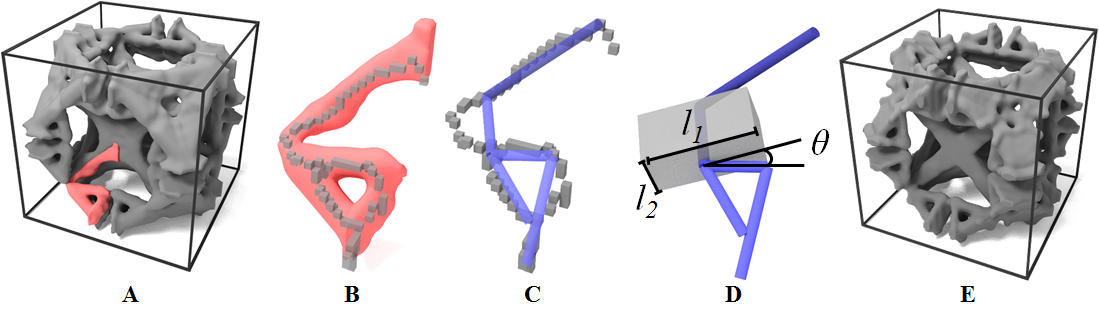
\includegraphics[width=0.95\textwidth]{images/skeletonExtraction.png}
	\caption{Steps for computing a microstructure template from a representative structure. For an input structure (a), we only need to analyze one tetrahedral slice (highlighted in red) of the whole structure due to its cubic symmetric construction. A morphological skeleton is extracted from the portion of the structure (b). The skeleton is a sequence of voxels. They are converted into a graph by connecting neighboring voxels. The graph is simplified (c) by merging paths into single edges while maintaining an error threshold. A cuboid (d) is placed on each edge of the simplified graph. (e) The final structure generated by the template using fitted parameters.}
	\label{fig:skelExtract}
\end{figure}

The final step of our software pipeline computes reduced parameters to facilitate intuitive navigation in the material property space.
Since the templates from the previous step contain tens of parameters that do not directly correspond to material properties, it is still difficult to understand the key design principles.
The reduced parameters allow for direct tuning of each material property.
For a given parametric template, its parameters are fitted to all structures of the corresponding family.
To avoid outliers, microstructures leading to large fitting errors ($>5\%$ voxel difference) are excluded.
Principal component regression (PCR) is then performed on the set of fitted template parameters to find principal directions in the template parameters space.
Varying the parameters in a direction corresponds to moving on the gamut boundary in a certain direction. A reduced parameter is assigned to each direction to control amount of change along that direction.
\subsection{Results and Discussion}
The results of this study focus on elastic material properties: Young's modulus, Poisson's ratio and shear modulus.
The elastic material property gamut is estimated from 15,000 3D cubic-symmetric microstructures at a voxel resolution of $64^3$.
The voxel resolution is a power of 2 because that is necessary to achieve optimal performance of our multigrid FEM simulation.
The specific resolution $64^3$ is chosen because it is sufficient for discovering auxetic structures with a wide range of relative shear modulus while $32^3$ structures cannot achieve comparable complexity or property ranges.
The macroscopic elastic parameter of each microstructure is computed using homogenization theory~\citep{Guedes1990,xia:2015:design} assuming a periodic boundary condition.
Each microstructure consists of a per-voxel binary material assignment. Due to manufacturing limits on minimum feature size,
sensitivity filter~\citep{sigmund:2007} is applied in gamut sampling step to avoid structures with overly thin features.
\begin{figure}
	\centering
	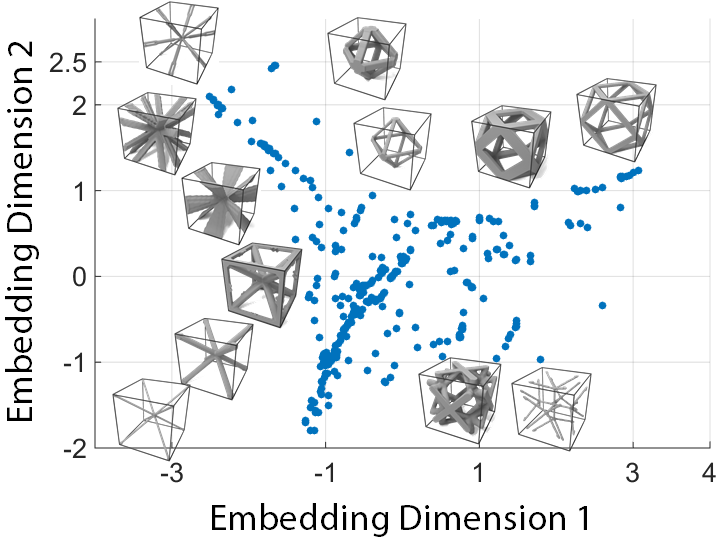
\includegraphics[width=0.5\columnwidth]{images/pprFamily.png}
	\caption{Structures with large Poisson's ratios ($\nu>0.3$). The embedding is computed using Isomap with 3 dimensions while the plot shows the 2D projection of the embedding. Structures with a positive Poisson's ratio have relatively simple topologies. Most structures are controlled by a single beam reflected according to cubic symmetry.}
	\label{fig:pprfamilies}
\end{figure}
\begin{figure}
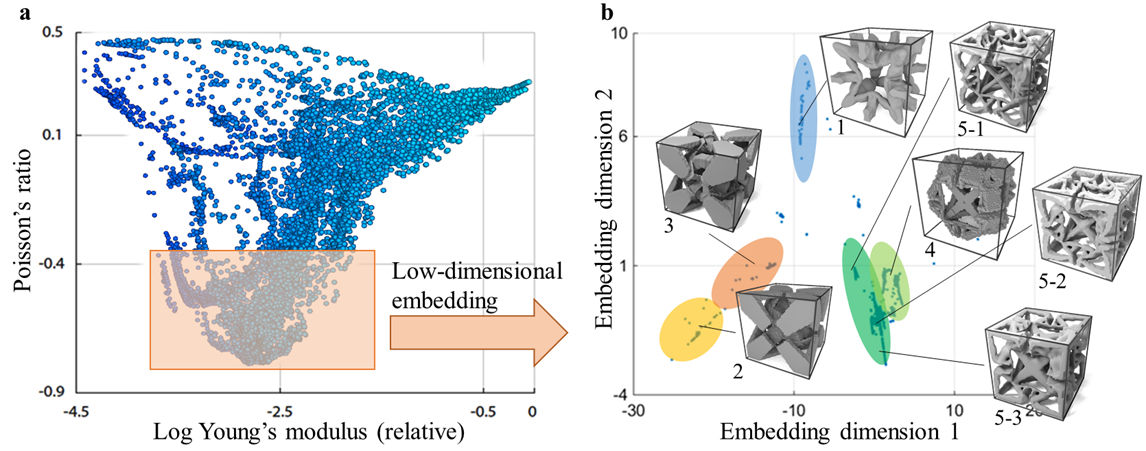
\includegraphics[width=0.95\columnwidth]{images/fiveFamilies.png}
\caption{Five microstructure families identified by nonlinear dimensionality reduction (NLDR). Structures with similar properties in the gamut (a) are selected to study their commonalities. We focused on structures with negative Poisson's ratio (auxetics) since they exhibit more complex structures. Auxetic families are identified in the embedding space numbered from 1 to 5 (b). Families with similar topologies are located closer in the embedding space. Three example structures from family 5 show underlying connection between seemingly distinct structures through gradual morphing of shape.}
\label{fig:families}
\end{figure}
Here we focus on analysis of auxetic structures since families with positive Poisson's ratios are relatively simple (Figure~\ref{fig:pprfamilies}). Five families with significant number of members (Figure~\ref{fig:families}) are discovered using three Isomap embedding dimensions. We confirmed that Isomap associates seemingly distant structures through intermediate structures. For example, structure 5-1 and 5-3 from family 5 have very different beam thicknesses resulting in large geometric distance. However, the embedding reveals that there is a sequence of structures such as 5-2 that make the connection between them.

Three structures with different material properties from each family are printed to verify simulation accuracy.
All structures are printed using an EOS SLS printer with elastic material PEBA2301.
The printer required a minimum feature size of $0.9mm$ for wire diameters and $0.8mm$ for wall thicknesses.
To satisfy the printing constraints, each cell is scaled to a side length of $2.54mm$.
Simpler structures from Template 1-3 are printed using a 2x2x2 grid arrangement while more complex families are printed using a 3x3x1 arrangement to allow support material to escape.
The base printing material is measured using an Instron 5944 with tensile tests instead of compression tests since a solid block of base material is too stiff for our equipment.
The Poisson’s ratio is measured using a video camera fixed on the test machine (Figure~\ref{fig:measure}).
Even though all samples are printed using the same printer and the same materials, the Young’s modulus of the prints is highly variable.
More specifically, the stiffest sample has a Young’s modulus which is twice as high as the one of the softest samples.
On the other hand, the Poisson’s ratio of the base print material is measured to be $0.34$ and has a much lower variance of $0.02$ in the sample set.
The 3D structures are measured using a compression test at a speed of $2mm/min$ with $6mm$ maximum strain.
The compression plates are lubricated with oil to reduce friction.
Significant variance in Poisson’s ratio is observed due to several factors in manufacturing and measurement.
An additional challenge is that the printer does not reliably reproduce the geometry specified by input files.
In practice, the printed models are thickened by $0.1-0.4mm$, which is significant compared to the thinnest feature size in our microstructures.
This stiffens the joints and reduces Poisson’s ratios.
The effect is exacerbated by incomplete support removal.
The support material is the same as the print material in powder form, which sticks to the print easily especially around hard-to-reach internal corners.
We believe that the discrepancy can be reduced in the future by using more precise printing technologies with soluble support material.
\begin{figure}
	\centering
	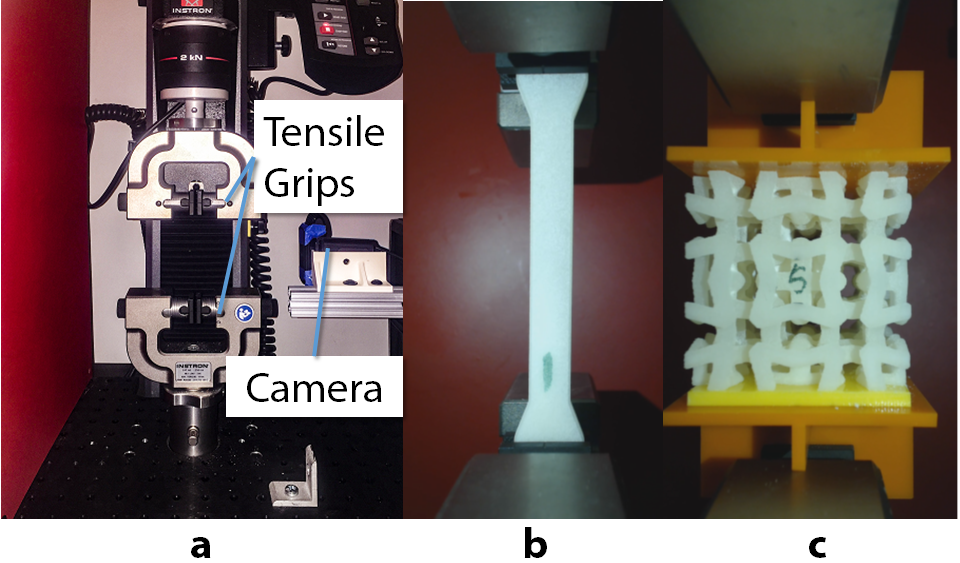
\includegraphics[width=0.5\columnwidth]{images/measure.png}
	\caption{Test apparatus (a) for measuring Young’s modulus and Poisson’s ratio using tensile (b) and compression (c) tests. The Poisson’s ratio is calculated using vertical displacements and horizontal displacements. The vertical displacement is read from both the tensile test machine and the camera for redundancy. The horizontal displacement is measured using the camera only.}
	\label{fig:measure}
\end{figure}
\begin{figure}
	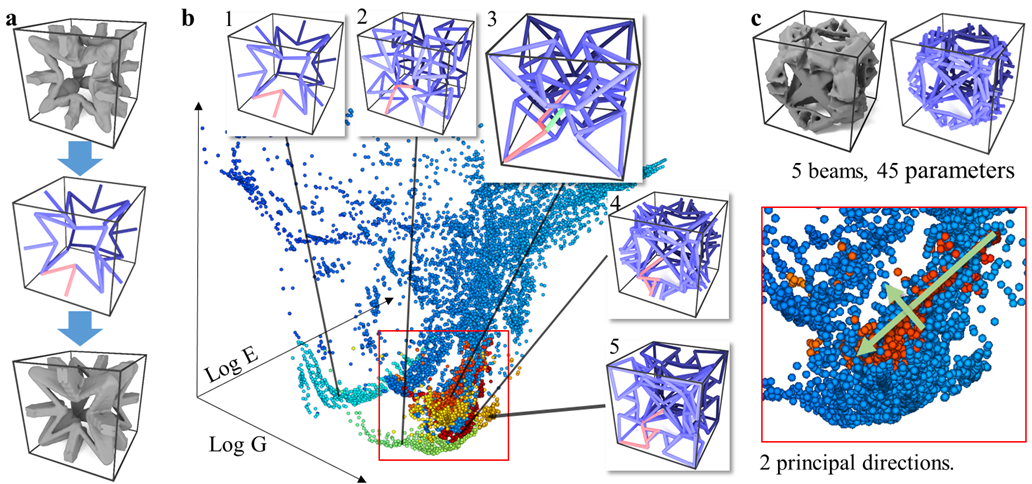
\includegraphics[width=\columnwidth]{images/mTemplates.png}
	\caption{Sampled coverage of microstructure templates in the gamut. (a) Extracting a skeleton (middle) from a representative structure (top). The skeleton represents the topology of the structure. A beam network is derived from the skeleton by placing a cuboid on each edge of the skeleton. Since we enforce cubic symmetry, the beams in a single tetrahedron determine the entire beam network. A template can generate a new structure (bottom) that approximates the original structure. (b) Coverage of each template in the material property space. (c) Reducing template parameter dimensions with principal component regression. The first two reduced parameters approximately correspond to varying the Young's modulus and Poisson's ratio of a structure. }
	\label{fig:mTemplates}
\end{figure}
For each of the five families, a parametric template is automatically constructed. The initial topology of a template is extracted from the morphological skeleton of a representative structure (Figure~\ref{fig:mTemplates}b). While the topologies are visually complex, they are generated by mirroring a small number of beams (highlighted in red) reflected according to cubic symmetry (Supplementary Table 2). The most complex template 5 contains only 6 control beams. The five families cover similar ranges of Young's modulus and Poisson's ratio. However, they span different ranges of shear modulus. Inspired by classical linear elasticity theory, we compare the shear modulus ratio defined as
\[
G'=\frac{2G(1+\nu)}{E},
\]
where $G$ is shear modulus, $E$ is Young's modulus and $\nu$ is Poisson's ratio. For traditional isotropic materials, the theoretical ratio is one. A low ratio indicates low resistance to shear deformation. For auxetic materials, lower ratios are much easier to obtain than higher ones. Even with foam structures assumed to be isotropic, experimental data from previous work indicates that the ratio is less than one~\citep{roh2013failure}.
\begin{figure}
	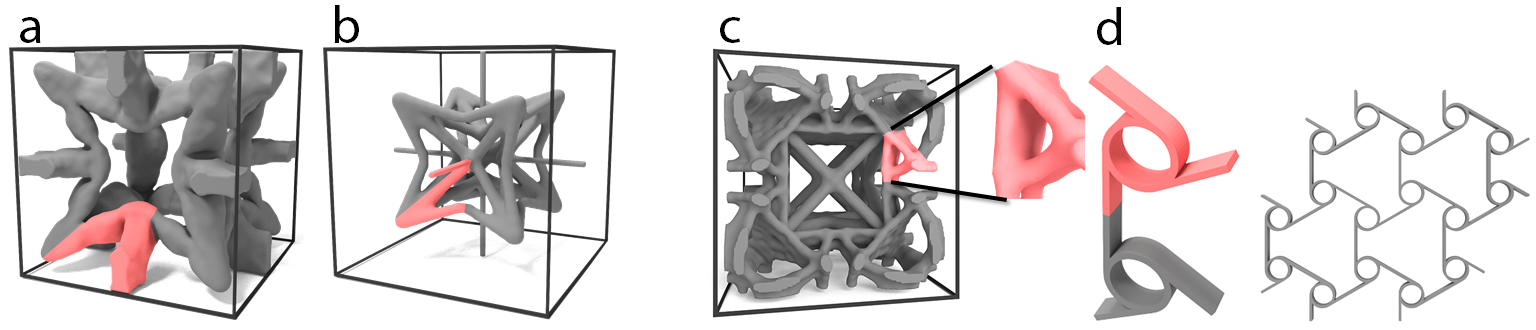
\includegraphics[width=0.9\columnwidth]{images/similarShape.png}
	\caption{Microstructures that resemble designs from previous works. (a) A reentrant structure in our database similar to the conceptual sketch (b) proposed by ~\citet{lakes1987foam}. Both structures have very low shear modulus ratio (0.05-0.15). Our structure is simpler with only two control beams reflected by cubic symmetry while (b) has three beams (highlighted in red). (c) The rotating triangle mechanisms resembles 2D chiral structures~\citep{prall1997properties}. (d) An anti-trichiral lattice~\citep{alderson2010elastic} has unit nodes most similar to our rotating triangle joints (highlighted in red).}
	\label{fig:similarShape}
\end{figure}
Template 1 resembles the conceptual sketch by~\citet{lakes1987foam} and belongs to the reentrant class of geometry. The difference is that our template has only two beams mirrored by cubic symmetry while Lakes' sketch contains three (Figure~\ref{fig:similarShape}). It is the simplest auxetic template that we identified, as our microstructure database does not contain any single-beam auxetic structure. The shear modulus ratio of this family falls in the range between 0.07 and 0.24, which is the lowest among all five families. Templates 2 and 3 are similar to each other and differ by a diagonal beam in the face center (highlighted in green in template 3). Since their geometric difference is small, they are adjacent in the Isomap embedding space. The central beam is responsible for increasing the shear modulus of the structures. For structures with $\nu$ around -0.5, the additional beam increases the maximum shear modulus ratio from 0.34 to 0.90. Templates 4 and 5 also differ by a single beam. Even the most complex template 5 is optimized from a simple cube frame through our continuous optimization step. The additional beam in template 5 makes the family stiffer overall compared to Template 4. Both families can achieve shear modulus ratio greater 1 for $\nu<-0.5$.

For each family, principal directions of template parameters are extracted using PCR. The templates and reduced parameters are included with the report. Two significant directions correspond to change in Young's modulus and shear modulus are kept for tuning structures. These directions reveal that for families 2 and 3, the thickness of the slanted column (Figure~\ref{fig:auxeticMech}a highlighted in red) is crucial for Poisson's ratio where the Poisson's ratio increases quickly with increasing beam thickness.
For families 4 and 5, the thickness of the rotating triangle affects the tradeoff between Young's modulus and shear modulus (Figure~\ref{fig:paramReduction}).
\begin{figure}
	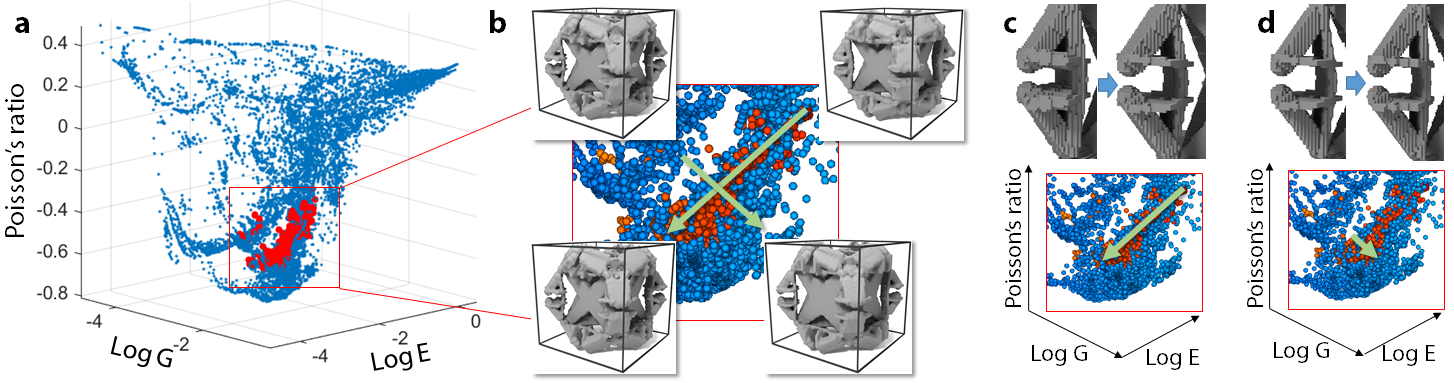
\includegraphics[width=\columnwidth]{images/paramReduction.png}
	\caption{Reduced parameters for Family 4. The distribution of the parameters corresponding to Family 4 is shown as red points in (a). The two principal directions are shown as green arrows in (b). The first direction reduces the Young's modulus and Poisson's ratio by decreasing the joint thickness (c). The second direction increases the shear modulus by slightly rotating the triangle joints outward (d).}
	\label{fig:paramReduction}
\end{figure}
While our cuboid-based templates are very simple, they are sufficient for replicating the auxetic behavior of the corresponding families.
We validated the auxetic properties of the fitted microstructures using simulation.
New structures are generated by varying template parameters.
300 new structures are sampled from each family along two PCR coordinate directions.
The coverage of the templates in the microstructure gamut (Figure~\ref{fig:mTemplates}b) shows that the templates can generate microstructures on the gamut boundary.

So far all of our simulations are carried out assuming linear elasticity, which is only accurate for infinitesimal deformations. We also make the common assumption that there is no self-collision. This assumption also imposes a limit on the maximum compressive strain we can apply to our structures before self-collision occurs. Representative structures from Families 4 and 5 have the lowest limit at $7\%$ compressive strain.
In practice, non-linear deformations such as bending and rotation are prevalent in our auxetic structures. Such deformations can cause linear elasticity to incorrectly predict significant volume expansion of rotated parts (up to $20\%$ percent in our test cases).
Thus, we tested our structures using a nonlinear material model to understand their behavior under large deformations.
We simulated nonlinear deformation behavior using Neo-Hookean material model.
At maximum allowed strain of $7\%$, linear elasticity and Neo-Hookean model still has acceptable agreement with an average error of $16\%$ in computed Poisson's ratio. In addition to simulation, we also printed three example structures from each family with varying Young's modulus and material ratio. Our structures demonstrated consistent auxetic behavior (Supplementary Video 3) even though they are optimized with linear elasticity assumption.
Our structures do not rely on structural instability~\citep{bertoldi2010negative} for auxetic behavior and shrinks uniformly as load increases.
This means that their deformations consistently follow the same pattern for different trials.

\begin{figure}
	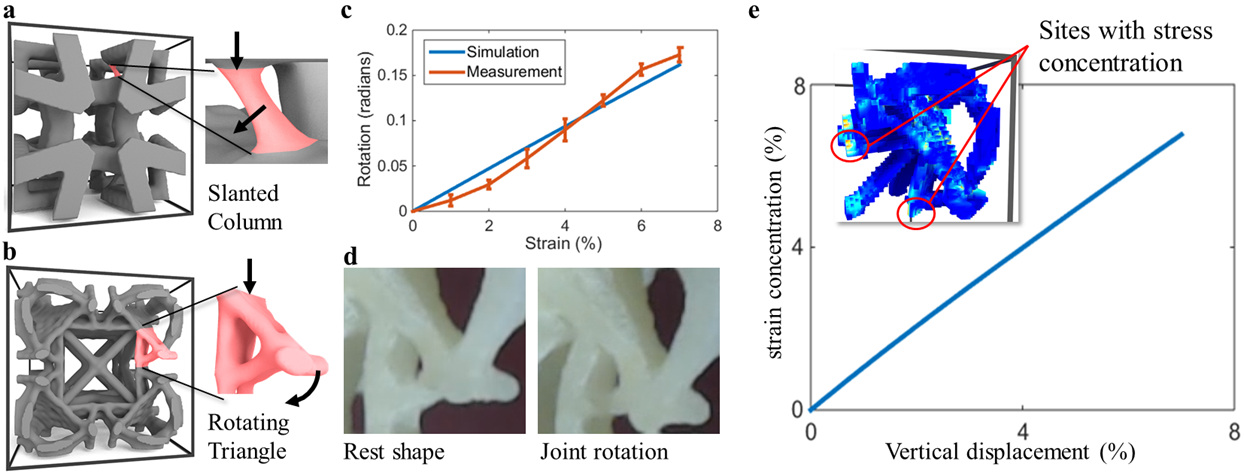
\includegraphics[width=\columnwidth]{images/auxeticMech.png}
	\caption{Discovered auxetic mechanisms. Two mechanisms capable of producing auxetic behavior are discovered from our microstructure families. The slanted column (a) transforms vertical stress into horizontal displacement. The rotating triangle mechanism (b) pulls the outer tip of the joint towards the center of the structure, reducing the macroscopic volume. (c) The relationship between vertical strain and rotation of the triangle joint. The rotation is observed in printed samples under vertical load (d). Stress is concentrated at the lower end of the triangle joint (e).}
	\label{fig:auxeticMech}
\end{figure}
Our process automatically discovered two types of auxetic mechanisms: slanted columns and rotating triangles (Figure~\ref{fig:auxeticMech}). The slanted column mechanism transforms vertical compression to horizontal motions. The rotating triangles transform vertical compression into a winding deformation that pulls the right end of the mechanism towards the center of the microstructure.
Their motions are shown in supplementary video S3.
While rotating triangles bear resemblance to existing 2D structures~\citep{alderson2010elastic} known as chiral structures (Supplementary Fig. 6d), its extension to 3D cubic structure with large shear modulus has never before been constructed. Additionally, the entire mechanism is discovered entirely automatically without imposing any artificial design restrictions---all microstructures are built from voxels. To inspire future applications of these mechanisms, we report the loading behavior of the mechanisms. These auxetic mechanisms are the most active parts in the microstructures. They act like joints that connect the more rigid scaffolding in microstructures. Because of this, they undergo the most deformation and concentrate a large amount of stress. For the rotating triangles, the stress is concentrated on the connections around the triangle. We computed the maximum principal strain in the structure with respect to the vertical compressive loading to provide insights into the strength of the block.
At the maximal compressive loading $(7\%)$, the maximum principal strain in the structure is $7\%$. Calculation using a reported Young's modulus of $80MPa$ yields a von Mises stress of $6.72MPa$ (Fig. 4e) while our print material has a reported strength of $8.5MPa$. The printed structures are approaching the strength limit under the load. Since the available material is relatively weak even compared to common materials such as ABS plastics and rubber, we believe that structural strength can be improved significantly with future manufacturing materials.

We have shown a computational method that combines discrete sampling, continuous optimization and dimensionality reduction methods for automatic discovery of new microstructure families and mechanisms that would have been challenging to design manually.
The discovered structures are suitable for manufacturing as they avoid thin features and distribute deformation over beams instead. They also span a wide range of shear moduli, allowing engineers to balance between different macroscopic properties. While our case study focuses on elastic material properties, the technique may be applied to other physical properties whenever predictive simulation exists. Our computational pipeline paves the way to discovery of structures that balance mechanical, thermal, optical, acoustic and electromagnetic properties. Moreover, it advances the understanding of underlying mechanisms that are crucial to extremal properties.

\section{Topology Optimization}
\label{sec:topoOpt}
A classic topology optimization problem consists of optimizing the shape and structure of a given object defined by a prescribed domain in order to minimize some cost function. For example, the standard topology optimization minimizes the compliance of the object while satisfying the static equilibrium and the total weight constraint.
Since the topology of the object is unknown {\it a priori}, a method of choice is to define the shape of the object through its material distribution and to locally work with material densities. To this end, the design layout is voxelized and a density variable is assigned to every cell of the discretized domain. By penalizing intermediate values for these densities, a binary distribution corresponding to the object's final layout can be eventually obtained.

In this work, we extend the traditional topology optimization algorithm in multiple ways.
First, we do not compute a binary material distribution at the cell level as commonly done. 
Instead, we leverage our database of microstructures and ask for each cell to be filled with one of the microstructures.
By doing so we change the topology of the object at a finer scale, i.e. within each cell. This is done by working with the macro-scale material properties of the microstructures instead of their geometry directly. The second difference is that our algorithm can be used with parametrizations of the material property space that are more complex than the single density parameter per cell that is commonly used in the standard topology optimization algorithm. Indeed, in our generalized topology optimization problem, each cell $c_i$ contains an n-dimensional material parameter $\bp_i\in \mathcal{R}^n$. We use $\bp$ to denote the stacked vector of material parameters in all cells.
Given a signed distance function $\Phi(\bp_i)$ that defines the gamut,
our new topology optimization problem is then written as
\begin{equation}
\begin{aligned}
\min_{\bp} : \quad & \mathcal{S}(\bp,\mathbf{u}) & \\
s.t. : \quad & \mathcal{F}(\mathbf{\bp},\mathbf{u})=0 & \\
: \quad & \Phi(\bp_i)\leq 0,  \quad 1\leq i \leq N_c&	
\label{eq:op}
\end{aligned}
\end{equation}
where $\mathcal{S}$ is a real-valued objective function that depends on the material parameters and the displacement vector $\bu$ of the entire object at the elasticity equilibrium.
The equality constraint $\mathcal{F}=0$ requires $\bu$ to satisfy the elasticity equilibrium and the inequality constraint $\Phi\leq0$ guarantees that the material properties of each cell stay inside the precomputed gamut.

In our examples, the material parameter $\bp$ consists of the density $\rho$ and the elasticity parameters $\be$.
We split our objective function into an elasticity term $\mathcal{C}(\vect{e},\bf u)$ that controls the deformation behavior (see Section \ref{sec:obj}) and an optional density term $\mathcal{V}(\rho)$ that controls the overall mass of the object.The density term can be written as
\begin{equation}
\mathcal{V}(\rho)=(\sum_{i=1}^{N_c}\rho_iV_i-\hat{M})^2\label{eq:vol},
\end{equation}
where $V_i$ is the cell volume and $\hat{M}$ is the target overall mass.
When one of the base material is void, the use of the density term allows to modify the topology of the object at a larger scale than the one of the microstructures, and thus to change the external shape of the object. 
In fact, even for multi-material designs involving base materials with similar mass densities, we noted that we could use the density term to encourage the presence of soft material in the structure. By removing the external cells entirely made of the soft material, we could then decrease the mass of the structure without significantly changing its mechanical behaviour.
Alternatively, the density term can also be used to control other quantities related to the ratios of the different materials such as the cost of the object.
For specific problems, we can also add spatially-varying weight control terms to Equation \ref{eq:vol}.
For example, we can control the target weight of each individual cell by adding a local term $(\rho_i-\hat{\rho}_i)^2V_i$.

Assuming static equilibrium, the elasticity constraint is written as 
\begin{equation}
\mathcal{F}(\mathbf{e},\mathbf{u})=K(\mathbf{e})\mathbf{u}-\bf f_{ext}=0,
\end{equation}
where $\bf f_{ext}$ are the external loads applied to the object.

The gamut constraint for a point $\mathbf{p}_i$ in the material property space is described by an $n$-dimensional level set function $\Phi(\mathbf{p})$.
We have $\Phi(\mathbf{p}_i)<0$ for a point inside the gamut, $\Phi(\mathbf{p}_i)>0$ for a point outside the gamut, and $\Phi(\mathbf{p}_i)=0$ for a point on the boundary of the gamut.
The value of $\Phi$ represents the $n$-dimension Euclidean distance to the level set boundary. %This distance can be linearly interpolated from the precomputed signed distance field.
The gradient of $\Phi$ are evaluated by a finite difference operation on the signed distance field.

We used a standard gradient-based numerical optimizer (Ipopt~\citep{ipopt} in our implementation) to solve Equation \ref{eq:op}. We enforced the elasticity equilibrium constraint using the adjoint method. The optimizer only needs to take the function values of $\mathcal{S}$ and $\Phi$ along with their gradients as input.

\subsection{Elasticity Objectives}\label{sec:obj}
We used two different types of objective functions for the elasticity term in our topology optimization algorithm. These two types of objectives allowed us to design a wide range of objects.
\paragraph*{Target Deformation}\label{sec:strain}
Our algorithm takes a vector of nodal target displacements and boundary conditions (external forces, fixed points, etc.) as input. Then, it automatically optimizes the material distribution over the object domain to achieve the desired linear deformation assuming a linear elastic behavior.

We define the deformation objective as
\begin{equation}
\mathcal{C}_d(\mathbf{e},\mathbf{u})=(\mathbf{u}-\hat{\mathbf{u}})^T \bD (\mathbf{u}-\hat{\mathbf{u}}),\label{eq:td}
\end{equation}
where $\hat{\mathbf{u}}$ is the vector of the target displacements, $\bf D$ is a diagonal matrix that determines the importance of each nodal displacement.	
We use $\bf D$ to define the subset of nodes that we are interested in.
For example, we can set most entries of $\bf D$ to zero and focus on a portion of the domain (see Figure \ref{fig:gripper}).

\paragraph{Minimum Compliance}\label{sec:compliance}
We have experimented with the same objective as the one used in the standard topology optimization algorithm where the compliance $\mathcal{C}_c$ is defined as
\begin{equation}
\mathcal{C}_c(\mathbf{e},\mathbf{u})=\mathbf{u}^T \bK(\mathbf{e}) \mathbf{u}.
\label{eq:mc}
\end{equation}
In the commonly used SIMP algorithm, the stiffness matrix $\bK_i$ of each cell $i$ depends on the artificial density value $\rho_i$
through an analytical formula such as $\bK_i = \rho_i^3\bK_0$ where $\bK_0$ corresponds to the stiffness matrix of the base material.
In contrast, the stiffness matrix in our objective function is directly computed from the material parameters of the material space and forced to correspond to a realizable material thanks to our gamut constraints.

Like in standard algorithms, we regularized the problem to avoid checkerboard solutions by applying a smoothing kernel on the material properties that favors smooth variations of the material parameters over the object layout.
Our optimizer supports multiple objectives by linearly combining weighted objective functions.
\section{Mapping Material Properties to Microstructures}
\begin{wrapfigure}{r}{0.2\linewidth}
 	\makebox[\textwidth][l]{\hspace{-0.4cm} 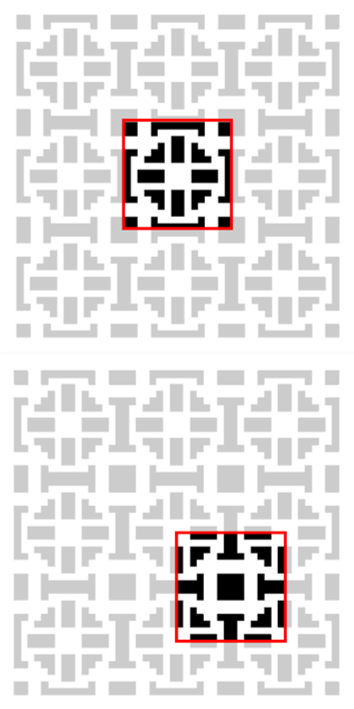
\includegraphics[width=1.0\linewidth]{images/TranslatedMicrostructureVertical.png}}
\end{wrapfigure}
After running the topology optimization algorithm, we generate a printable result by replacing each cell in the object lattice by a microstructure whose material properties match the optimal ones.

Material properties of the microstructures are computed using the homogenization theory which is more accurate with a smooth transition between the geometries of neighboring cells.
While smoothness in the material parameters can be easily enforced, it does not imply topological similarity of nearby microstructures. 
For example, any translation of a given microstructure in a periodic tiling will result in a microstructure geometrically different but with exactly the same mechanical properties. 
Fortunately, our database is very dense and multiple microstructures generally map to similar points in the material property space, offering several variants. To further increase the number of possibilities, we also incorporate an additional exemplar for each microstructure by translating it by half its size, which preserves its cubic or orthotropic symmetry without changing its properties (see inset Figure). We then run a simple but effective algorithm that picks the microstructure exemplars that minimize the boundary material mismatch across adjacent cells. We quantify this mismatch by $\mathcal{I}=\sum_{i=1}^{N_c} \mathcal{I}_i$, where $\mathcal{I}_i$ is the contribution associated to the cell $i$ and corresponds to the number of boundary voxels filled with materials that are different from the ones of the voxels' immediate neighbours across the interfaces.

Our algorithm proceeds as follows:
\begin{itemize}
\item For each cell, we define a list of possible candidates by picking all the microstructures mapping to material points lying in the vicinity of the optimal material point and we randomly initialize the cell with one of the candidates.
\item We compute the mismatch energy $\mathcal{I}_i$ associated to each cell $i$ and sort the cells according to their energy. 
\item We pick the first cell in the sorted list, i.e. the one with the highest energy and assign to it the microstructure candidate that decreases the energy the most. If we cannot decrease the cell energy, we move to the next cell in the list.
\item We update the mismatch energies of all the impacted cells and we update the priority list.
\item We repeat the last two steps until the mismatch energy $\mathcal{I}$ cannot be decreased anymore.
\end{itemize}

\section{Results and Discussion}
We first analyzed our microstructure sampling algorithm for 2D and 3D microstructure gamuts. Then we used these precomputed gamuts and we designed and optimized a wide variety of objects with our topology optimization algorithm.
\subsection{Microstructure Sampling}
We evaluated our method on two- and three-dimensional microstructures made of one or two materials. For the 2D case we considered patterns with cubic and orthotropic mechanical behaviors that can be described with 4 parameters (3 elasticity parameters and density) and 5 parameters (4 elasticity parameters and density) respectively. In 3D we computed the gamut corresponding to cubic structures with 4 parameters. In all cases, the size of the lattice for the microstructures was set to 16 in every dimension. We used isotropic base materials whose Young's modulus differed by a factor of 1000 and having 0.48 as Poisson's ratio. We initially computed the databases for two-material microstructures, but also adapted these databases for microstructures made of a void and a stiff material. In the later case, we replaced the softer material by void, filter out all the microstructures with disconnected components and, in the 3D case, filled the enclosed voids and recomputed the homogenized properties. We provide a comparison between the initial and postprocessed databases in the supplementary material. The resulting postprocessed gamuts are also depicted in Figure \ref{fig:gamuts}. 
Our databases contain 274k, 388k and 88k 2D cubic, 2D orthotropic and 3D cubic microstructures respectively and took from 15 hours to 93 hours to compute, which correspond to 68, 19 and 5 sampling cycles, respectively.
\begin{figure}
	\centering
	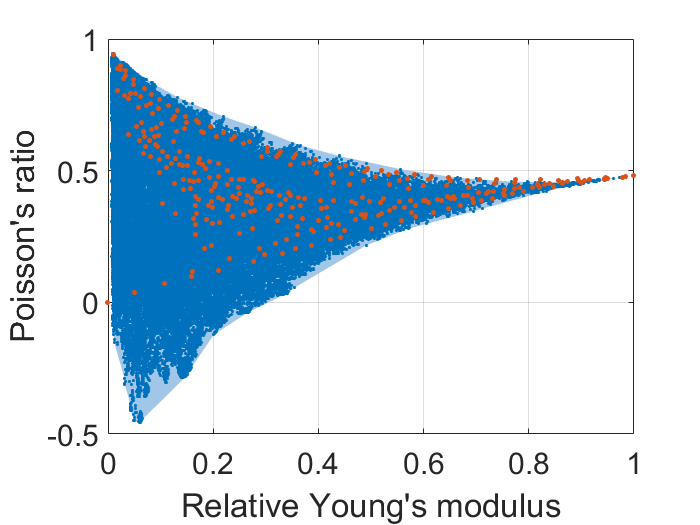
\includegraphics[width=.24\linewidth]{images/2D_cubic.png}
	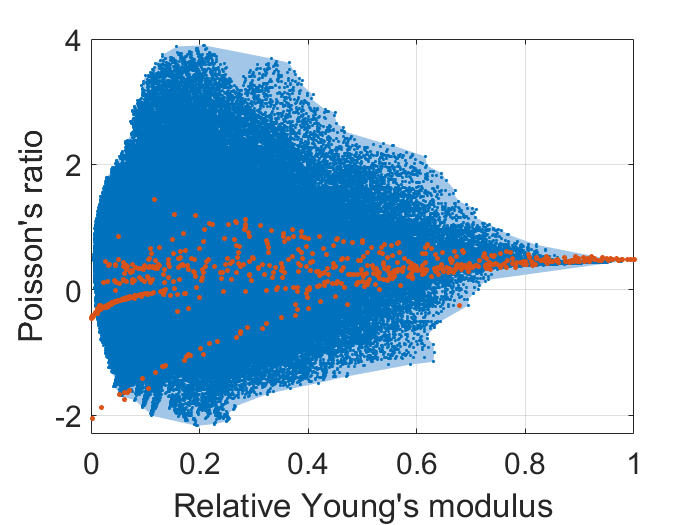
\includegraphics[width=.24\linewidth]{images/2D_ortho.png} 
	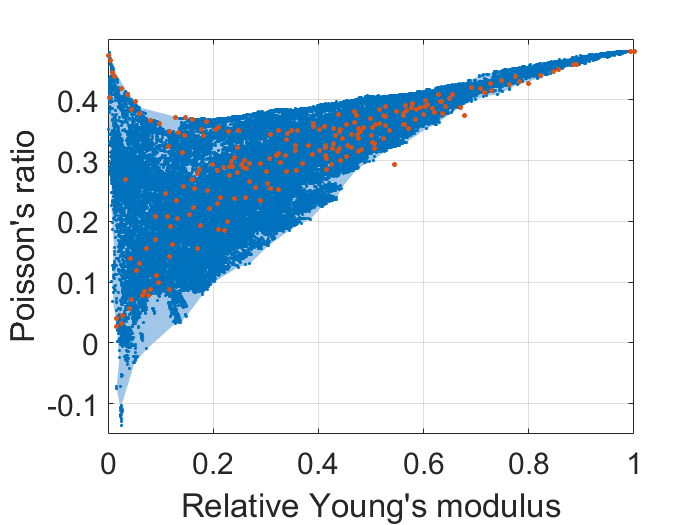
\includegraphics[width=.24\linewidth]{images/3D_cubic.png}
	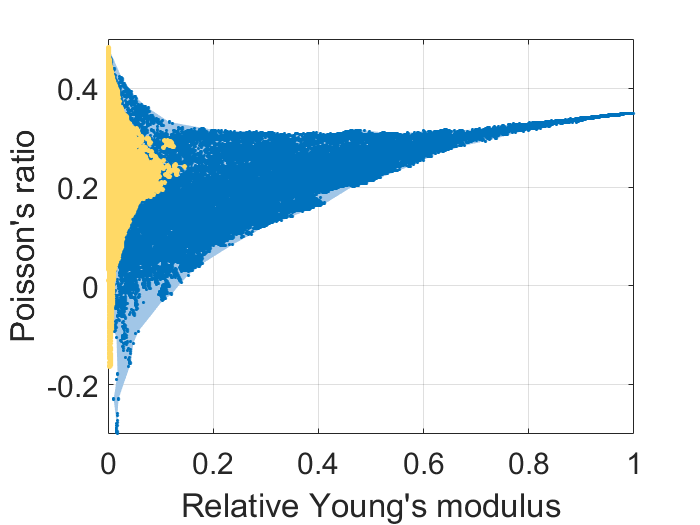
\includegraphics[width=.24\linewidth]{images/3D_cubic_Panetta.png}
	\caption{Gamuts computed with our discrete-continuous sampling scheme for 2D cubic structures (\emph{left}) , 2D orthotropic structures (\emph{second from left}), 3D cubic structures (\emph{second from right}) and 3D cubic structures with 0.35 as Poisson's ratio (\emph{right}). The plots show the results for the projection of the gamuts on the plane defined by the macroscale Young's modulus along the x axis (normalized by the Young's modulus of the stiffest base material) and the Poisson's ratio corresponding to a contraction along the y-direction when the material is stretched along the x-direction.
		The blue dots correspond to the generated samples,the orange dots correspond to the microstructures from~\citet{Schumacher:2015} and the yellow dots correspond to the microstructures from~\citet{Panetta:2015}.}
	\label{fig:gamuts}
\end{figure}
We first compared our results to the ones obtained by~\citet{Schumacher:2015}
and observed a significant increase in the coverage of the material space, even for 2D microstructures where we used a coarser discretization. This comforts us with the idea that topology optimization only, while helpful to locally improve the microstructure geometries, is suboptimal when one aims to discover the entire gamut of physical properties. The diversity of the microstructures that we obtained is also much richer, thus providing a larger set of options for the practical use of microstructures. Note that they employed some regularization to avoid thin features. For $16^3$ microstructures, we found regularization unnecessary since they are manifold and have a minimal feature size  of 1/16 of the lattice size, which is the same order of magnitude as the thinnest parts of Schumacher's microstructures.
For completeness, we also compared our database of 3D microstructures to the one of~\citet{Panetta:2015} at $16^3$ and $64^3$ grid resolutions (Figure \ref{fig:gamuts}, \emph{right}). Our initial database was computed with 0.48 as Poisson's ratio and is shown in the supplementary material. For this comparison, we then recomputed the material properties of the microstructures using the same Poisson's ratio as Panetta's, i.e 0.35, which affects the extremal values of the obtained gamut.
For the $64^3$ microstructures, we used morphological operations in the discrete step and sensitivity filtering with a radius of 3 voxels in the continuous step to limit the minimum feature size to 1/32 of the lattice size~\citep{sigmund:2007}. Note that this comparison is provided for reference only since our microstructures are cubic while Panetta's are isotropic (a subset of cubic). Furthermore, they target a different 3D printing technology with self-supporting constraints not imposed here.
Finally, we also obtained a dense sampling in the interior of the space, as a result of the randomness inherent to our approach. This reduces the need of running costly optimization in these areas and occurs even if we do not explicitly enforce any sampling there.

We also experimented with three-material 2D cubic microstructures (two solid materials with Young's moduli differing by a factor of 1000 and with 0.48 as Poisson's ratio, plus a void material). The resulting database contains about 800k microstructures that can potentially be printed. The corresponding gamut and some examples of the generated microstructures are shown in Figure \ref{fig:Cubic2D_3Materials}.
\begin{figure}
	\centering
	\includegraphics[width=.5\linewidth]{images/Cubic2D_3Materials.png}
	\caption{Gamut corresponding to 2D cubic microstructures made of two materials and void. The Young's modulus of the microstructures is plotted using a logarithmic scale. We show above some examples of microstructures lying near the estimated boundary of the gamut, i.e. with extreme material properties. The dark color corresponds to the softer material, while the light grey color is used for the stiffer material.}
	\label{fig:Cubic2D_3Materials}
\end{figure}
\subsection{Topology Optimization}
We tested our topology optimization algorithm on a number of simple test cases and large scale examples. Detailed analysis and discussion of the results is provided below.

\paragraph{Impact of the Material Space}
We evaluated the impact of the chosen material space on a 2D cantilever beam with optimized minimum compliance. We tested our topology optimization algorithm on isotropic, cubic and orthotropic gamuts as well as with the virtual materials used in the traditional SIMP approach and for which the stiffness of the material $E=\rho^p E_0$, $p \geq 1$ is a function of the density $\rho$ of the cell and the stiffness of the base material $E_0$. We also tested our algorithm on an analytical gamut with allowed stiffnesses $E$ defined by $E\leq \rho^3 E_0$. The results are shown in Figure \ref{fig:defo_cvg}. It can be noted that, as the dimension of the material space increases, the final energy of the system decreases. This is to be expected since higher dimensional space means larger gamuts.
Thus, when using cubic materials, the minimum compliance objective function reaches 3\% lower energy than the standard SIMP method with power index 3.
This difference reaches 11\% when we use orthotropic materials.
It is worth noting that the lowest elastic energy is achieved when we use the traditional SIMP method with $p=1$ (as shown in Figure \ref{plot:cvg}). However, this solution does not correspond to a realizable structure since some of the optimized materials do not correspond to any microstructure.
\begin{figure}
	\centering
	\includegraphics[width=0.95\textwidth]{images/cantilever.png}
	\caption{Material property distributions optimized in the orthotropic (\emph{top left}), cubic (\emph{bottom left}), isotropic (\emph{top middle}) and an analytically defined gamut $E \geq \rho^3 E_0$ (\emph{bottom middle}), with the material property space dimensions ranging from five to two. 
		We compare our algorithm with the standard SIMP method with power index $p=1$ (\emph{top right}) and $p=3$ (\emph{bottom right}). For these figures, we computed the color of each cell by mapping every base vector of the normalized parameter space to a color range and linearly interpolating the colors associated to each of the parameters.
		In this example, the left side of the cantilever is fixed while a force distribution is applied to the bottom side (see red arrows in the top left picture).}
	\label{fig:defo_cvg}
\end{figure}

\begin{figure}[h]
	\centering
	\includegraphics[width=0.95\textwidth]{figs/cvg_test.png}
	\caption{Convergence tests. Variation of the objective energy (\emph{left}) and the elastic energy \emph{right} of a beam being optimized for minimum compliance as the optimization progresses. The convergence plots correspond to the beam of Figure \ref{fig:defo_cvg} when optimized using different material spaces (\emph{top}), different resolutions for the beam lattice (\emph{middle}) when using cubic microstructures, and different initial material properties for the cubic microstructures (\emph{bottom}).}
	\label{plot:cvg}
\end{figure}
\begin{figure}
	\centering
	\includegraphics[width=.5\linewidth]{images/bar_visio_new.png}
	\caption{
		Optimizing a beam to take an ``S'' shape under compression.
		A beam with homogeneous material can only compress uniformly (left column).
		The optimized beam can deform as requested (right column).
		Target displacements are set on the horizontal boundary cells.
		The color plot for the bottom beams shows the deformation error of each cell defined by Equation~\ref{eq:td}.
		\label{fig:beam_S_shape}}
\end{figure}

\paragraph{Matching Quality}
	We evaluated for different examples the matching quality of the target deformation optimization.
	For the first test, we forced a beam to take an `S' shape when undergoing tensile forces (Figure \ref{fig:beam_S_shape}). In order to avoid overfitting, we applied target displacements on the vertices of the boundary cells only. As depicted in the figure, the use of microstructures largely improves the global shape of the beam, which closely matches the target deformed shape. This becomes even more striking when compared to the behavior of a beam made of a homogeneous material.
		We also validated our algorithm by designing a soft ray whose wings can flap using a compliant mechanism (see Figure \ref{fig:ray} and accompanying video). Boundary conditions are applied on two circular areas located along the spine of the ray. Each disk has one degree of freedom for deformation, namely contracting or expanding along the disk normals. This mechanism resembles the one of many hydraulics-driven soft robots. We define two target deformation objectives corresponding to the flapping of the wings up and down, when alternatively contracting and expanding the two disks' boundaries. By running our multi-objective topology optimization framework, we can compute an optimized material design that can achieve both deformation modes when the corresponding boundary conditions are exerted.

\begin{figure}[t]
	\centering
	\includegraphics[width=.6\linewidth]{images/ray.png}
	\caption{Designing a soft ray. The wings of the ray flap up and down when cells on its spine contract and expand.
	Constrained vertices are colored in green.
	The deformations achieved with the optimized materials are displayed on the bottom row.}
	\label{fig:ray}
\end{figure}
\paragraph{Convergence and Robustness}
We evaluated the convergence rate of our topology optimization both on the minimum compliance problem and with the target deformation objective. For the minimum compliance problem, we used the same loading as the one of Figure \ref{fig:defo_cvg}. The corresponding results are shown in Figure~\ref{plot:cvg} where we plot both the deformation energy of the structure as defined in Equation \ref{eq:mc} and the original objective of the problem \ref{eq:op} that also includes the volume term defined by Equation \ref{eq:vol}. For all these examples, the algorithm converged after a couple of dozen iterations, irrespectively of the lattice resolution, i.e. the number of variables and the number of non-linear constraints. This demonstrates the scalability of the our algorithm. We also tested the robustness of our algorithm by starting with different initial conditions. In this case, we initialized the material parameters of each cell with a random material point projected onto the boundary of the gamut. Similar to other topology optimization schemes, we have no guarantee that we reach the global minimum of the function, and indeed, our algorithm sometimes converges to different solutions. However we note that these different solutions have a similar final objective value and are therefore equally good.

For the evaluation of the target deformation optimization, we tested the convergence rate when optimizing for functional mechanisms.
To this end, we designed several grippers that can grasp objects by moving their tips when external forces are applied to their extremities. We experimented with four sets of boundary conditions, namely, pulling and pushing the back of the gripper horizontally, and compressing and stretching the extremities of the gripper vertically. As shown in Figure \ref{fig:gripper}, these different settings lead to different material structures. The deformation errors of all the four designs converge to a low level after a couple of hundreds of iterations.

\begin{figure}
	\centering
	\includegraphics[width=0.9\linewidth]{images/gripperVar.png}
	\includegraphics[width=0.4\linewidth]{images/gripper4_L2.pdf}
	\includegraphics[width=0.4\linewidth]{images/gripper4_Linf.pdf}
	\caption{Designing functional grippers. The left column shows the rest shape of the gripper and the target deformation for the tip.
	The green dots correspond to the fixed vertices while the blue arrows are the target displacements.
	The middle and right columns correspond to the optimized results obtained for the specified boundary conditions.
	The inset pictures color-code the initial and final deformation error for the different examples.
	The convergence plots in the bottom row depict the change in the sum of the deformation errors corresponding to all the cells (left) and the value of the maximal cell error contribution (right) as the optimization progresses.}  
	\label{fig:gripper}
\end{figure}
\paragraph{Accuracy}
\begin{figure}
	\centering
	\includegraphics[width=.6\linewidth]{images/hom_beam.png}	
	\caption{Comparison of simulated beams with homogenized material properties (\emph{inset pictures}) to the ones using full microstructures (\emph{large pictures}).
		}\label{fig:hom_beam}
\end{figure}

\begin{figure}[h]
	\centering
	\includegraphics[width=.8\linewidth]{images/hom_cube_random.png}	
	\caption{Comparison of simulated cubes with different material patterns modeled by homogenized cells (\emph{inset pictures}) and full resolution microstructures (\emph{large pictures}).}
		\label{fig:hom_cube_2}
\end{figure}

We evaluated the accuracy of our algorithm on several optimized structures by comparing the deformation obtained when using the optimized homogenized material properties for each cell to the one obtained by a high resolution simulation in which every cell is replaced by its mapped microstructure.
We first evaluated the accuracy on a deformable bar, one side of which was rigidly attached while the other was subject to different sets of external conditions (see Figure \ref{fig:hom_beam}). We used a $8\times2\times2$ lattice to represent the bar with homogenized cells, which translates into a $128\times32\times32$ grid for the full resolution mesh. Similar stretching, bending and shearing behaviors were obtained for both sets of models. From a quantitative point of view, the differences amount to 5-10\% in terms of average vertex displacement and 9\%-33\% in terms of elastic deformation energy (see Table \ref{tab:hom}). We further evaluated the effects of material patterns by running a similar comparison on a cube made of periodic layers of similar microstructures and with random assignments of microstructures (Figure \ref{fig:hom_cube_2}).  As reported in Table \ref{tab:hom}, we show that the ratio between the magnitudes of the average vertex displacement differences is between 4\% and 7\%, and the elastic energy difference is between 10\% and 19\%.

Finally, we also compared the behaviors of one of the grippers (Figure \ref{fig:gripper_validate}). The original optimized gripper is made of 3k elements while the high resolution version is made of 4M voxels.
Overall, the two models exhibit similar global deformation behaviors, in particular in the tip area. Some differences can be observed on the left side of the gripper for which the high-resolution model exhibits a lower effective material stiffness than its homogenized counterpart. With the same displacement boundary conditions applied, the high-resolution model deforms about 25\% more than the homogenized model.
	
	\begin{figure}[t]
		\centering
		\includegraphics[width=.6\linewidth]{images/gripper_cmp.png}	
		\caption{Comparison of a simulated gripper with homogenized material properties (\emph{inset picture, left}) to the one using full microstructures (\emph{main picture, left}). The figures on the right show the vector field of vertex displacement of the two models. The blue-to-red colors represent the magnitudes of the displacements.}
			\label{fig:gripper_validate}
	\end{figure}
	
	\begin{figure}[h]
		\centering
		\includegraphics[width=.8\linewidth]{images/hom_cube_peri.png}	
		\caption{Simulation of a cube made of a periodic arrangement of a single microstructure at different resolutions. Inset pictures correspond to the model with homogenized material properties, while main pictures correspond to the full resolution simulations.}
			\label{fig:hom_cube_1}
	\end{figure}
	
The differences observed between the homogenized model behaviour and the full resolution simulation can be explained by two major factors: (i) numeral stiffness when using larger elements which tends to make the homogenized mesh slightly stiffer in particular when bending deformation arises, (ii) violation of the periodicity assumption when replacing each cell by a single microstructure. This issue can be reduced by replacing each cell by a {\it tiling} of microstructures. This was verified on a cube made of a periodic arrangement of a single microstructure (see Figure \ref{fig:hom_cube_1}). And indeed, as we increase the resolution of the simulation grid, the error between the homogenized model and the full resolution version decreases and converges to similar values.

\paragraph{Orthotropic materials}
We tested the behavior of our algorithm in a 5-dimensional space by using the gamut of 2D orthotropic microstructures depicted in Figure \ref{fig:gamuts} (\emph{middle}). To this end, we used a regular lattice whose vertices on the left side where fixed and we applied parallel forces on the vertices of the opposite side. The goal in the test was to minimize the compliance of the structure. As can be seen in Figure \ref{plot:res} and in the accompanying video, we experimented with different force directions. Unsurprisingly, when a single cell is considered, the microstructure that we obtain has a structure that is aligned with the direction of the forces (see Figure \ref{plot:res}, \emph{left}). 
For a higher resolution lattice this is no longer true and the resulting overall structure becomes less intuitive (see Figure \ref{plot:res}, \emph{right}). 
Note that the resulting material distribution varies smoothly. By considering various alternative for each material point, our tiling algorithm is able to map the material properties to microstructures which are well connected. 

\begin{figure}
	\centering
	\includegraphics[width=0.95\textwidth]{images/ortho_square.png}
	\caption{Optimizing the orthotropic material parameters of a single cell (\emph{left}) and a $32\times32$ lattice of cells (\emph{right}) subject to directional forces. The vertices on the left side of the layout are fixed while forces are applied on the right vertices as depicted by the red arrows. Our simple but effective tiling algorithm allows to nicely transition between microstructures of smoothly material properties (\emph{right, top}).}
	\label{plot:res}
\end{figure}

\begin{table}
	\centering
	\footnotesize
	\caption{Error statistics (SI units). The size of one microstructure is set to $1\times1\times1$.}
	{\begin{tabularx}{\linewidth}{ |X| X | X | X | X | }
			\hline
			Example & Mean displacement & Mean displacement difference & Elastic energy \newline homogenized & Elastic energy \newline full resolution\\ \hline
			Beam 1 & 6.47$\times10^{-3}$ & 6.04$\times10^{-4}$ & 6.85$\times10^{-5}$ & 6.17$\times10^{-5}$ \\
			Beam 2 & 6.47$\times10^{-3}$ & 6.04$\times10^{-4}$ & 1.63$\times10^{-5}$ & 1.08$\times10^{-5}$ \\
			Beam 3 & 5.07$\times10^{-3}$ & 4.97$\times10^{-4}$ & 2.38$\times10^{-4}$ & 2.07$\times10^{-4}$ \\
			Beam 4 & 8.78$\times10^{-3}$ & 4.45$\times10^{-4}$ & 3.33$\times10^{-4}$ & 2.30$\times10^{-4}$ \\
			Cube 1 & 3.62$\times10^{-3}$ & 2.86$\times10^{-4}$ & 3.64$\times10^{-3}$ & 3.20$\times10^{-3}$ \\
			Cube 2 & 4.35$\times10^{-3}$ & 1.94$\times10^{-4}$ & 6.82$\times10^{-3}$ & 5.94$\times10^{-3}$ \\
			Cube 3 & 5.42$\times10^{-3}$ & 4.22$\times10^{-4}$ & 7.81$\times10^{-3}$ & 6.32$\times10^{-3}$ \\
			Gripper& 1.32$\times10^{-2}$ & 6.90$\times10^{-3}$ & 8.67$\times10^{-3}$ & 5.70$\times10^{-3}$ \\
			Cube 4 & 5.22$\times10^{-3}$ & 4.89$\times10^{-4}$ & 2.08$\times10^{-2}$ & 1.63$\times10^{-2}$ \\
			Cube 5 & 5.21$\times10^{-3}$ & 2.17$\times10^{-4}$ & 1.89$\times10^{-2}$ & 1.63$\times10^{-2}$ \\
			Cube 6 & 5.21$\times10^{-3}$ & 1.32$\times10^{-4}$ & 1.82$\times10^{-2}$ & 1.63$\times10^{-2}$ \\
			\hline
		\end{tabularx} }
		\label{tab:hom}
	\end{table}
	
	\subsection{3D-Printed Designs}
	
	Leveraging our two-scale approach, we used our topology optimization algorithm to generate a wide variety of high resolution models that we 3D-printed. We used a Stratasys Objet Connex 500 and the two base materials \emph{Vero Clear} and \emph{Tango Black Plus} and used the database containing the three-dimensional cubic microstructures. The sizes and computation times of the resulting models are outlined in Table \ref{tab:results}. 
	
	Since Ipopt performs a line search at each gradient step, one single step may correspond to multiple simulations. We show the average time required for taking a step in the last column of Table \ref{tab:results}. For these large scale examples, Ipopt takes two hundred iterations in average to find a local minimum. 
	Since our problem is formulated as a very general constrained continuous optimization, it is independent of the optimization package that is used and its speed could potentially be further improved by using alternative minimizers. 
	We found Ipopt to be a good choice for its capability to efficiently handle a large number of inequality constraints, which is not the case of other popular minimizers used in topology optimization such as the method of moving asymptotes (MMA).
	
	Our algorithm is mainly directed towards engineering applications and targets the design of objects undergoing small deformations. In the following examples, we sometimes intentionally exaggerated the target displacements (and scaled the external forces accordingly) for better visualization, which does not change the output of the algorithm with a linear material model.
	
	\begin{table}
		\centering
		\footnotesize
		\caption{Statistics on the 3D-printed models. The last row uses the database of $64^3$ microstructures.} 
		{
			\begin{tabularx}{\linewidth}{ |X| X | X | p{3cm}| p{3cm}| }
				\hline
				Example & Grid Size & \# Voxels & Time per FEM Solve [s] & Time per Step [s]\\ \hline
				Beam   & 96$\times$24$\times$4  & 38M  &  0.7 & 5\\
				Flexure & 32$\times$32$\times$16 & 67M  & 1 & 12\\
				Gripper   & 64$\times$32$\times$8  & 67M  & 1.7 & 10\\	\hline
				Bunny & 32$\times$32$\times$32 & 134M  & 0.6 & 4 \\
				Bridge & 128$\times$64$\times$32 & 1074M  & 27 & 81\\
				Bridge 2 & 320$\times$160$\times$80 & 1074G  & 1.3k & - \\
				\hline
			\end{tabularx} }
			\label{tab:results}
		\end{table}
		
		\paragraph{Beams with controlled deformation behaviour}
		We started by designing a 3D hollowed beam with a desired deformed shape. The beam was stretched by moving vertices on two opposite sides. Our topology optimization algorithm was run using a target deformation objective. The resulting optimized material properties and the 3D-printed structure are depicted in Figure \ref{fig:beam}. 
		\begin{figure}[h!]
			\centering
			\includegraphics[width=.8\linewidth]{images/bar2_two.png}
			\caption{
				An optimized hollow beam with target deformation. The left figure shows the target deformation and optimized material distribution. The right figure shows the 3D-printed structure and the achieved deformation.
				\label{fig:beam}}
		\end{figure}
		\paragraph{Multi-Objective Flexure Design}
		We tested our algorithm on a multi-target deformation setting by optimizing the structure of a flexure mount with two different target shapes (see Figure \ref{fig:flexure}). Here, our goal is to design a flexure that resists vertical loads while remaining compliant to horizontal loads. We assume that the object mounted on the flexure is connected to the flexure using a cylindrical connector that transmits the forces to the flexure via the connecting area. In the first scenario, vertical forces are applied to the points of the cylindrical area and we ask the flexure to stay as close as possible to its rest configuration. In the second scenario, horizontal forces are applied to the points of the cylinder and we ask the flexure shape to match the shape shown in the Figure \ref{fig:flexure}. 
		\begin{figure}
			\centering
			\includegraphics[width=.6\linewidth]{images/flex_four.png}	
			\caption{Optimizing a flexure mount. The flexure is connected to an object thanks to a cylindrical connector. We leave space for this connector by keeping a cylindrical area of the design layout empty of material. The material distribution of the flexure is optimized for two sets of external forces applied to the cylindrical area. Under vertical load, the flexure should stay close to the rest shape while under horizontal load, the flexure should deform according to the inset figure.}
				\label{fig:flexure}
		\end{figure}
		\begin{figure}[h]
			\centering
			\includegraphics[width=.6\linewidth]{images/gripper_print.png}
			\caption{3D-printed functional grippers. By setting different target ratios of the rigid material, different designs can be obtained. 
				When more soft material is used the grasping behavior of the gripper is obtained via out-of-plane bending (\emph{top}), whereas more rigid material is used, the gripper deformation remains planar (\emph{bottom}).} 
			\label{fig:gripper_printed}
		\end{figure}
		\paragraph{Gripper}
		We verified the functionality of our grippers by fabricating two of them. For these results we ran the optimization on high resolution meshes of the version that grasps the object when the extremities of the gripper are pressed (see Figure \ref{fig:gripper_printed}). By changing the parameter controlling the ratio of the soft material, different designs based on different mechanisms can be achieved. When more soft material is used the gripper achieves its target deformation thanks to out-of-plane bending, while for stiffer designs, the grasping motion is achieved via in-plane deformation.
		\paragraph{Minimal Compliance Examples}
		To demonstrate the scalability of our algorithm, we ran our topology optimization algorithm on a Stanford bunny (Figure \ref{fig:bunny}) made of more than 100 million voxels and subject to two load case scenarios.
		We also designed two bridges of increasing resolutions. The first bridge was optimized using a lattice of half a million cells which corresponds to 1 billion voxels (Figure \ref{fig:top_bridge}). For the second bridge, we used the database of $64^3$ microstructures and a layout made of 4 million cells, which amounts to 1 trillion voxels. We initialized the topology optimization by running the algorithm on a lower resolution grid with 1.4 million elements and used the resulting parameters as initial material parameter values for the higher resolution optimization. 	
		\begin{figure}
			\centering	
			\includegraphics[width=.6\linewidth]{images/bunny_two.png}
			\caption{Stanford bunny optimized for two loading cases. Two sets of external forces are applied to the back and chest of the bunny as indicated by the arrows, and the color indicates the material distribution (\emph{left}). Material parameters are mapped to microstructures to obtain an object that can be actually printed (right).
				\label{fig:bunny}}
		\end{figure}
		\begin{figure}
			\centering
			\includegraphics[width=.6\linewidth]{images/bridge_three.jpg}
			\caption{Optimizing a bridge. The initial layout corresponds to a 128x64x32 regular grid. We apply uniform loads on the upper plane deck. We compute the material parameters and set cells with extremely low stiffness to void (\emph{top left}). We look up the microstructures and 3D print the bridge (\emph{top right}). We scaled the problem to 1 trillion voxels by using a lattice of 4 million elements where each element corresponds to a $64^3$ microstructure (bottom).}
				\label{fig:top_bridge}
		\end{figure}
\chapter{Designing Dynamic Mechanisms}
\label{ch4:desdyn}
The realistic simulation of highly-dynamic elastic objects is important for a broad range of applications in computer graphics, engineering and computational fabrication. However, whether simulating flipping toys, jumping robots, prosthetics or quickly moving creatures, performing such simulations in the presence of contact, impact and friction is both time consuming and inaccurate. In this paper we present Dynamics-Aware Coarsening (DAC) and the Boundary Balanced Impact (BBI) model  which allow for the accurate simulation of dynamic, elastic objects undergoing both large scale deformation and frictional contact, at rates up to 79 times faster than state-of-the-art methods. DAC and BBI produce simulations that are accurate and fast enough to be used  (for the first time) for the computational design of 3D-printable compliant dynamic mechanisms. Thus we demonstrate the efficacy of DAC and BBI by designing and fabricating mechanisms which flip, throw and jump over and onto obstacles as requested.
\section{Introduction}

We present a pair of new methods to accurately simulate geometric and material nonlinearities subject to frictional contact, large loads and high-speed collisions at rates significantly more than an order-of-magnitude faster than previously available.
Our methods combine efficiency and accuracy to enable design-for-fabrication optimization. They can be used for both fast, realistic animation and engineering analysis. 

Here we look towards a new generation of efficient mechanisms for practical \emph{dynamic} function~\citep{Lipson:2014fa,Rus:2015eq,Reis:2015hb,Reis:2015ey}. In order to extend physics-driven computational design to this domain, however, a bottleneck must be overcome - the physical simulation itself. Simulations must accurately replicate the behavior of elastic materials subject to high-speed, transient dynamics. Modeling these systems combines many of the remaining grand challenges in simulating elastica. Specifically we must accurately resolve nonlinear elasticity, large deformations, stiff materials, high-speed dynamics, rapid loading and unloading, frictional contact, internal friction, high-speed collisions, and rebound. 

State-of-the-art FEM systems currently able to accurately match these effects are exceedingly expensive - runtimes on the order of days are standard to perform a single simulation in many cases~\citep{Belytschko:2013tz}. 
Thus, while generating a single simulation for visualization or animation is already time consuming, the many simulations required during design optimization compound an already prohibitive computational burden.
\subsection{Efficiency with Accuracy}
Let us explore four potential solutions for constructing fast \emph{and} accurate simulation algorithms: (1) higher-order elements, (2) adaptive meshes, (3) reduced models, and (4) numerical coarsening. Can these methods provide the necessary efficiency to enable design-optimization while obtaining the predictive accuracy required to match fabricated results?

\emph{Higher-order elements} offer us the opportunity to replace thin regions of our models with elements that capture higher-order deformation modes. While an attractive strategy, this poses two challenges. 
First, due to changing design parameters, we will need to identify suitable regions on-the-fly in order to perform this replacement. 
Second, coupling swapped-in higher-order elements to other element types introduces overhead. Consider, for example, replacing lower-order hexahedra with plate elements in these regions. We must then ensure continuity of displacements between plate-like portions of the design and thicker, volumetric portions.
This, in turn, requires introducing difficult coupling constraints~\cite{Bergou2007,Martin:2010:USE}. Finally, even with such additional efforts, these substitutions may not always improve computational performance as high-order elements contain more DoFs than their low-order counterparts~\cite{Belytschko:2013tz}. 

\begin{figure}
	\centering
	\includegraphics[width=0.7\columnwidth]{./figs/Adaptive_Meshing}	
	\caption{Comparing adaptivity and coarsening. A tetrahedral model of a jumper is adaptively remeshed to capture input stress fields from its launch and landing states. We compare the resulting element and node counts to our DAC-coarsened model. We set the minimum edge length for remeshing to one that was experimentally found to yield convergent numerical results.}
	\label{fig:adaptiveMeshing}
\end{figure}

\emph{Adaptive meshing} allows us to reduce element counts in material regions where refinement is less critical.
Let us ignore the difficulty of implementing adaptive meshing and the per time step cost to remesh. Even so, adaptive meshes are challenging in our setting. We model objects that undergo rapidly changing boundary conditions and globally varying stress fields due to contacts, loading and impacts. Adaptive meshing in our setting must then, necessarily, feature high numbers of elements to capture these details. See Figure~\ref{fig:adaptiveMeshing}. Here, using our experimentally validated, accurate element edge length as adaptive meshing threshold, our tetrahedral mesh contains 6.5X to 28X more nodal DoFs than our corresponding DAC-coarsened mesh. The DAC-coarsened mesh is likewise simpler to implement and has no per time step computational cost. 

\emph{Reduced models} utilizing linear modes~\cite{James:2002:DDR,Hauser:2003:IDU} are widely applied to accelerate dynamic simulations. The key issue here is that linear modal models provide only a \emph{linear} approximation of the deformation space leading to inaccurate linearization artifacts, 
such as swelling during rotation;
see Figure~\ref{fig:modalModels}. Optimized quadrature approaches, in turn, can afford efficient integration of non-linear forcing functions, but do not alleviate these artifacts~\cite{An:2008:OCE} when relying on an underlying modal deformation space.
Finally, nonlinear modal models~\cite{Barbic:subspace:2005} can alleviate some of these issues but so-far remain challenging to incorporate in the design process in comparison to their linear counterparts~\citep{Chinesta2013}. 

\begin{figure}
	\centering
	\includegraphics[width=0.7\columnwidth]{figs/Modal_Expansion}
	\caption{Linear modal models suffer from distortion as deformations grow. In (a) we illustrate increasing deformations, left to right, with corresponding inflation errors. Even for smaller deformations, (a) middle, the linear modal model still introduces significant distortions leading to modeling inaccuracies. In (b), left, we overlay simulations of small deformation  performed respectively with the linear modal model (red) and the coarsened nonlinear FE model (grey); and, on the right, evaluate accuracy of the modal model. During simulation, even these smaller deformations introduce inaccuracies in the modal model due to element inflation; here up to 13.7\%.} 
	\label{fig:modalModels}	
\end{figure}

We begin by observing that \emph{numerical coarsening} offers an exciting alternative for efficient yet predictive FE modeling. Coarsening methods effectively apply coarse resolution FE meshes as reduced DoF models and then seek material models that reproduce the behavior of a high-resolution FE counterpart. Analytical solutions for coarsening have been developed for linear material models (models where the stress varies linearly with strain)~\cite{Kharevych2009,Nesme2009,Torres:2016:HIC}.
Due to this linear assumption, and similarly to the linear modal models discussed above, we find them difficult to apply for the accurate modeling of the nonlinear materials required for 3D-printed objects.
Unfortunately, while coarsening offers promise, prior work, to our knowledge, does not account dynamic effects, inertial properties, nor material damping characteristics.
As we see in Figure~\ref{fig:coarse}, this causes even the nonlinear DDFEM to produce highly inaccurate dynamic simulations.
\begin{figure}
	\centering
	\includegraphics[width=0.7\columnwidth]{figs/DDFEM.pdf}	
	\caption{Dynamics-oblivious coarsening is significantly inaccurate for dynamic simulation. Left: two twisted elastic bars, initialized to the same configuration, are time-stepped in a dynamic simulation with an energy based, data-driven coarsening (DDFEM) model (blue) and a high-resolution FEM mesh (green). Right: small localized errors in the material model of the DDFEM simulation aggregate across the mesh over time to quickly produce large global errors when compared to the high resolution solution.}
	\label{fig:coarse}
\end{figure}
Building on the promise of coarsening techniques and inspired by recent developments in frequency matching for plausible computer animation~\cite{Li:2014:SEE,BinWang:2015fx}, we develop a new, dynamics-aware coarsening (DAC) method that, in contrast to prior approaches, provides well-over an order-of-magnitude performance enhancement, while maintaining fabrication-level accuracy when modeling highly dynamic motions subject to frictional contact. Our method does so without complex substructuring, does not require adaptive remeshing, accounts for dynamic effects including damping, and does not introduce prohibitive linear modeling artifacts and so is applicable to a wide selection of nonlinear constitutive models for 3D-printed materials.  

\subsection{Impact Response for Elastic Materials}
Even with a suitably accurate FE solution to model \emph{material} dynamics, accurate impact response for elastic materials on collision remains highly challenging.  To capture the bounces and rebounds of elastic mechanisms coming into contact with the ground - consider for example the heel strike of a sneaker - we need to get this right. State-of-the-art, implicit time-stepping methods for FEM with contact solve variational forms of time-steppers, e.g., variational Implicit Newmark, subject to additional, fully implicit contact and friction forces~\cite{Kane:1999kr,Pandolfi:2002ik}. 
These form so-called nonsmooth or \emph{complementarity} integrators. 


\begin{figure}
	\centering
	\includegraphics[width=0.8\columnwidth]{figs/Figure_2_BBI}	
	\caption{Comparison of complementarity Newmark integration, DKE Stabilization and our BBI model for the impact resolution of an elastic, 3D-printed block. BBI closely matches the maximum rebound height achieved by the experimental result while both the Complementarity and DKE methods overestimate the rebound significantly.}
	\label{fig:BBI_block_compare}
\end{figure}

However, these complementarity integrators have two well-known flaws~\cite{Deuflhard:2008fu}: (1) these methods can yield spurious oscillations on the contact boundaries and (2) the effective impact response of these methods is too energetic. Effectively the normal velocity on impact along the elastic boundary should be dissipated completely. Instead, complementarity methods with Newmark will generate an entirely incorrect elastic restitution; see Figure~\ref{fig:BBI_block_compare}. To address these problems~\citet{Deuflhard:2008fu} introduced the now-standard DKE contact-stabilization step to filter contact response with projection. In the limit, DKE makes the impact-response model consistent,
while in FE codes it is applied as an effective strategy to recover from the well-known limitations of implicit integration with impact. However, it remains widely acknowledged that the right-way to accurately model high-speed collision response with implicit FE remains an open question at this time - not only in graphics - but more broadly in scientific computing as well. As an example consider Figure~\ref{fig:BBI_block_compare} where we see that both the complementarity model \emph{and} the DKE filter produce different but equally incorrect predictions of the response of a stiff elastic block dropped on the floor. Here we offer a new, Boundary-Balancing Impact (BBI) model for FE that gains us accurate prediction of impact response for the stiff 3D-printed materials we focus on here; see Figure~\ref{fig:BBI_block_compare}.

\subsection{Summary and Contributions}
High-fidelity simulation methods for elastodynamics are too slow for use in fabrication design tasks while existing strategies to reduce the simulation cost of elastica (including adaptive, reduced and coarsened models) are too inaccurate and/or too expensive to employ. Finally, existing FE models for simulating elastic collision and rebound miss critical compliance coupling in the filter stage.

We have exposed and analyzed the limitations of simulation methods for the predictive modeling of elastodynamics at rates sufficient for fabrication design optimization. Next, we develop our \emph{Dynamics-Aware Coarsening} (DAC) method to address this need {(\S3)}. DAC jointly identifies \emph{and} predictively simulates fabricated materials. To address current limitations in FE collision-response filtering we then introduce our \emph{Boundary Balancing Impact} (BBI) model {(\S4)}. 
We then validate these contributions by comparing simulated results generated by DAC and BBI with real-world results experimentally obtained from a range of compliant 3D-printed jumping and throwing mechanisms that flip, throw projectiles, jump onto obstacles and jump over walls (\S5).
\section{Simulation Preliminaries}
\begin{figure}
	\centering
	\includegraphics[width=0.99\textwidth]{images/dynPhase.png}
	\caption{Bottom: the dynamic behavior of a 3D-printed, elastic jumping mechanism in experiment. Top: our DAC-coarsening combined with our BBI impact model generate a simulation that predictively captures this experimental behavior at rates 79X faster than state-of-the-art FEM.}
	\label{fig:simulationStage}
\end{figure}
\label{sec:simPrelim}
Accurate time-varying tracking of energy dissipation is key to accurate dynamic simulation~\cite{Marsden:2001dj} and so we rely on implicit Newmark time integration, a discrete variational integrator~\cite{Kane:2000dw} with consistent high-quality energy tracking. 
We experimented with other integrators, including linearly implicit Newmark, Implicit Euler, and BDF2, but found them to be wanting in either stability or energetic behavior; see our Supplemental for details.
\subsection{Discrete Model} We begin with a standard elastic material model for 3D printed materials.
To capture stiff elastic response of 3D-printed materials we use the neo-Hookean material model, augmented with Rayleigh damping to capture transient dissipation of vibrations, and discretize with second order, hexahedral finite elements. We start with a second-order, implicit Newmark %($\gamma=1/2,\beta=1/4$) 
time discretization 

\begin{align}
\vc M \vc \delta^{t+1} &= \vc b^t +  \tfrac{h^2}{4} \vc F(\vc q^{t+1}) -\tfrac{h^2}{4} \vc D(\vc q^{t+1}) \vc v^{t+1},
\label{eq:newmark_free}
%
\end{align}
\begin{align}
\begin{split}
\vc q^{t+1} &= \vc q^t + \vc \delta^{t+1},\\
\vc v^{t+1} &= \tfrac{2}{h} \vc \delta^{t+1} - \vc v^t,
\end{split}
\label{eq:newmark_free_update}
\end{align}
where
\begin{align}
\vc b^t = h \vc M \vc v^t + \tfrac{h^2}{4} \vc F( \vc q^t) -\tfrac{h^2}{4} \vc D( \vc q^t) \vc v^t,
\label{eq:newmark_predictor}
\end{align}
$h$ is the timestep size, $\vc F(\cdot)$ is the internal force vector, $\vc D(\cdot) = a \vc M + b \vc K(\cdot)$, 
with $a,b \in \mathbb{R}^+$ is the Rayleigh damping matrix, $\vc M$ is the stiffness-consistent mass-matrix~\citep{Belytschko:2013tz},
$\vc K(\cdot) = -\nabla \vc F(\cdot)$ is the tangent stiffness matrix, 
and $\vc q, \vc v \in \mathbb{R}^{3n}$ are respectively the nodal position and velocity vectors. In the absence of dissipative forces this method is symplectic and momentum preserving~\citep{Kane:2000dw}.
With dissipation we find that integration gives us accurate bookkeeping of system energy at comparable cost to implicit Euler. 

\subsection{Material Parameters}
No matter how good our energy bookkeeping, the overall fidelity of our method is critically determined by the accuracy of the material parameters we select. While many material parameters are reported in the literature, there remains large and significant variation in these values across 3D-print batches, printing orientations and curings; see \S5.
For predictive simulation we need to identify these values. In addition, we must model dissipation requiring us to determine unreported damping properties; e.g., $a$ and $b$ in the Rayleigh model. Finally, as discussed below and complicating matters even further, these material parameters are discretization dependent at non-convergent spatial resolutions. In the next section we will detail our DAC model to capture dynamic deformation, stiffness and damping at coarsened spatial resolutions.

\subsection{Contact and Friction} For contact we need to model nonpenetration constraints and frictional contact forces that resist sliding along interfaces. 
Contacts are between object parts or between a part and a fixed boundary such as the ground.  At each time step we apply continuous collision detection to the predicted trajectory to gather contact constraints into a contact set $\mathcal C$. 

To simplify the following, for each such contact $k \in \mathcal C$, the relative acceleration between material points $\vr x_i$ and $\vr x_j$ (at contact $k$) can be expressed via the map $\vc \Gamma_k: \dot{\vc q} \rightarrow \dot{\vr x}_i - \dot{\vr x}_j$. See our Supplement
for details on construction of $\vc \Gamma_k$. If $\vr y \in \mathbb{R}^3$ is a force applied to point $\vr x_i$, and an equal but opposite force is applied to point $\vr x_j$, then $ \vc \Gamma_k ^T \vr y$ is the resulting generalized force applied to the contacting system.

In turn, points in contact apply an equal and opposite force along their shared, unit-length normal $\vr n_k \in \mathbb{R}^3$.  In global coordinates this is equivalent to applying a force of magnitude $\bar{\alpha}_k \in \mathbb{R}^+$ along a generalized normal 
\begin{equation}
\vc n_k = \vc \Gamma_k^T \vr n_k \in \mathbb{R}^{3n},
\end{equation}
to the system. The subspace of generalized normal directions
\begin{equation}
\label{eq:N}
\vc N = (\vc n_1 ... \vc n_{|\mathcal C|})
\end{equation}
then forms a basis for contact forces. Concatenating the corresponding force magnitudes in  
$\alpha = (\bar{\alpha}_1, ..., \bar{\alpha}_{|\mathcal{C}|})^T$, the total contact force applied in the system is then $\vc N \alpha$. 

Friction forces lie in the tangent plane orthogonal to the contact normal. At each contact $k$ we sample an orthogonal pair of unit length vectors from the tangent plane. The $3\times2$ matrix composed column-wise of these samples is given by $\vr T_k$ so that a friction force, $\vr f_k \in \mathbb{R}^3$, applied at a contact $k$, lies in the span of $\vr T_k$ with $\vr f_k = \vr T_k \bar{\beta}_k$, where each $\bar{\beta}_k \in \mathbb{R}^2$ gives the frictional response coefficients at contact $k$.

The total friction force applied to the system at each contact $k$ must be equal and opposite and is $\vc f_k = \vc \Gamma_k^T \vr T_k \bar{\beta}_k$. 
The generalized basis for a friction force at contact $k$ is then 
\begin{equation}
\vc T_k = \vc \Gamma_k^T \vr T_k \in \mathbb{R}^{3n \times 2}.
\end{equation}
We build the corresponding subspace of generalized tangent directions,
\begin{equation}
\vc T = ( \vc T_1 ... \vc T_{|\mathcal C|})
\end{equation}
and form the corresponding vector of frictional force coefficients as $\beta = ( \bar{\beta}^T_1,  ... , \bar{\beta}^T_{|\mathcal C|})^T$.
The total friction force on the system is then $\vc T \beta$.

Contact and friction forces can be inexpensively modeled explicitly~\citep{Belytschko:2013tz} but this introduces instabilities and nonphysical oscillations on boundaries even at small time step for stiffer materials~\cite{Deuflhard:2008fu}. Thus FEM state-of-the-art generally turns to implicit time-integration for efficient contact force modeling. 

\citet{Kane:1999kr} proposed the now standard nonsmooth-Newmark method for contact modeling. 
This is a fully implicit time-stepping model that couples frictional contact with internal energies and forcing in each solve.
\begin{align}
\begin{split}
\vc M \vc \delta^{t+1} &= \vc b^t +  \tfrac{h^2}{4} \vc F(\vc q^{t+1}) -\tfrac{h^2}{4} \vc D(\vc q^{t+1}) \vc v^{t+1} + \tfrac{h^2}{2} \vc N \alpha +  \tfrac{h^2}{2}  \vc T \beta.
\label{eq:newmark_contact_implicit}
\end{split}
\end{align}
Note that here, unlike internal forces, contact forces are evaluated solely at the time step endpoint to ensure dissipation.
Next, to fully define the time stepper, consistency conditions are required for contact and friction forces. 

Enforcing the complementarity model for contact requires contact forces to balance along boundaries 
\begin{align}
\begin{split}
0 \leq \alpha \perp \vc N^T \delta^{t+1} \geq 0,
\label{eq:contact_conditions}
\end{split}
\end{align}

Friction in turn is modeled with the {\em Maximal Dissipation Principle}, requiring friction to maximize the rate of negative work done at each contact, $- \vr f_k^T \dot{\vr x}$. The total dissipation performed by friction is then 
\begin{align}
\sum_{k \in \mathcal{C}} \bigl(- \vr f_k^T \dot{\vr x}_k \bigr) =  -\Bigl[\sum_{k \in \mathcal{C}} \vr f_k^T  \vc \Gamma_k \Bigr] \dot{\vc q} =  - \beta^T \vc T^T \dot{\vc q}.
\end{align}
Then, maximizing the Coulomb-constrained dissipation simultaneously at \emph{all} contact points, with the implicit Newmark discretization~\cite{Pandolfi:2002ik}, gives us the final condition for our numerical integration
\begin{align}
\begin{split}
\min_{\beta} \{ \beta^T \vc T^T (\tfrac{2}{h} \delta^{t+1} - \vc v^t) : \mu_k \bar{\alpha}_k \geq \|\bar{\beta}_k\|, \> \forall k \in \mathcal{C} \},
\label{eq:max_diss_transform}
\end{split}
\end{align}
where $\mu_k$ is the local friction coefficient at contact $k$.

Taken together stepping this implicit \emph{complementarity} Newmark integrator with (\ref{eq:newmark_predictor}), (\ref{eq:newmark_contact_implicit}), (\ref{eq:contact_conditions}), (\ref{eq:max_diss_transform}) and (\ref{eq:newmark_free_update}) provides predictive simulation at slower speeds of contact. For higher speed contacts and impacts, the remaining challenge lies in stabilizing contact stresses, velocities and displacements~\cite{Deuflhard:2008fu} to ensure that simulated objects' bounces and rebounds consistently match with their real-world counterparts. 
In Section \ref{sec:BBI} we will address this issue with a new impact model for FE simulation. First, however, we address our fundamental scaling problem: how can we gain 
accurate dynamic simulation without being bottlenecked by systems too large to solve quickly per time step?
\section{Dynamics-Aware Coarsening}
\label{sec:DAC}
We couple numerical coarsening with parameter acquisition.
Our DAC method computes \emph{numerical} stiffness parameters for the nonlinearly elastic, Neohookean material model, and damping parameters for the Rayleigh damping model so that, when applied to the coarsened simulation mesh, the dynamic behavior of a high-resolution simulation is preserved.

\begin{figure}
	\centering
	\includegraphics[width=0.95\columnwidth]{images/modeFit.png}
	\caption{Dynamics-aware coarsening (DAC) coarsens meshes to capture deformation with calibrated stiffness. We observe FE meshes capture accurate deformation modes up to a quite coarse resolution. However, these same coarse meshes suffer from numerical stiffening (see Figure~\ref{fig:numerical_stiffness}). We design coarse mesh FE models by matching both significant deformation modes (above) and their captured material response (see Figures~\ref{fig:error} and \ref{fig:vibration_match}) to obtain efficient and predictive coarse-mesh FEM simulations of dynamics. }
	\label{fig:defo_and_frequency_match}
\end{figure}

Because the goal of DAC is to replicate the dynamic behavior of a high-resolution simulation, we focus on creating a coarse mesh which captures both the large-scale deformation modes, and the corresponding natural frequencies of the high-resolution mesh. We do this in two stages. First, we produce a coarse hexahedral mesh that can replicate the large scale deformation modes of our high-resolution mesh. Second, we compute material and damping parameters that yield matching fundamental frequencies for each mode shape on this coarse mesh.

\begin{figure}
	\centering
	\includegraphics[width=0.7\textwidth]{figs/stiffness.pdf}
	\caption{Static Deformation Test. We apply an identical load to three meshes with the same model geometry. With the same material parameters, a high-resolution mesh (left) is effectively 2.5x softer than the corresponding coarse mesh (right). Applying our captured numerical Young's modulus to the coarse mesh (middle) regains the correct deformation of the original, high-resolution mesh on the left.}
	\label{fig:numerical_stiffness}
\end{figure}

\subsection{Geometric Coarsening}
DAC uses an iterative procedure {to create the} coarse mesh while maintaining mode shapes. We initialize our mesh to a coarse hexahedral discretization of the starting geometry, $\vc q^0$, and then subdivide recursively until we reach a convergent mesh resolution. We then solve the generalized mass-PCA system 
\begin{align}
\vc K(\vc q^0) \vc q = \lambda \vc M \vc q
\end{align}
for the dominant shape modes of the convergent system and then coarsen via bisection 
with mass-PCA until we reach a maximally coarse mesh that matches the dominant four shape modes to tolerance. We use a relative geometric difference of $5\%$ (Hausdorff distance) as our tolerance threshold. Typically this is a short validation step as even the coarsest meshes generally satisfy this criteria (Figure~\ref{fig:defo_and_frequency_match}).

\subsection{Material Parameter Fitting}  
Our geometric coarsening ensures that our DAC mesh captures significant deformation modes of our design accurately. However, when simulated, these same coarse meshes suffer from \emph{numerical stiffening} -- an increase in effective stiffness and damping as a consequence of decreased mesh resolution; see Figure~\ref{fig:numerical_stiffness}. This leads to unacceptably inaccurate simulated trajectories no matter how we simulate this system. Regaining predictive stiffness and damping by refining the discretization would take us back to intractable mesh sizes; see Figure~\ref{fig:adaptiveMeshing}.
Rather than refine, we keep our coarse mesh (as we have already ensured that our geometry is resolved there) and instead calibrate its frequency spectrum to directly match experiment. 

To do this, we rescale our coarse model stiffness so that its fundamental frequency matches an observed frequency. As we will see below, this simple analysis sufficiently recovers effective stiffness and damping to regain a predictive 
nonlinear simulation with our coarse mesh. 

From the geometric coarsening step above, we retain the numerical eigenvalues, $\lambda_i^0$, of our coarse mesh with corresponding deformation modes $m_i$ approximated linearly by the damped harmonic oscillator~\cite{shabana:2012} 
\begin{align}
\ddot m_i = -(a + b \lambda_i ) \dot m_i - \lambda_i m_i,
\end{align}
or equivalently 
\begin{align}
\begin{split}
m_i(t) = &A_i\exp(-d_i t)\sin(2 \pi f_it+ \theta_i),\\
&f_i = \frac{1}{2\pi}\sqrt{\lambda_i - (\frac{a+ b \lambda_i}{2})^2},\\
&d_i=\frac{1}{2}(a + b \lambda_i),
\label{eq:oscillator}
\end{split}
\end{align} where $a$ and $b$ are Rayleigh Damping parameters and $\lambda_i$ is the $i^{th}$ eigenvalue associated with the $i^{th}$ deformation mode.

\begin{figure}
	\centering
	\includegraphics[width=0.6\columnwidth]{images/calibrationfig.png}
	\caption{Top: tracking the oscillations of a 3D-printed calibration rig allows us to measure mesh-dependent stiffness and damping parameters. Bottom: the resulting DAC-simulated frames at corresponding times for visual comparison to the captured motion.}
	\label{fig:calibrationRig}
\end{figure}

We then 3D-print calibration rigs with tracker markings, see e.g., Figure~\ref{fig:calibrationRig}, and capture high-speed video (240 fps) of the rigs vibrating.  
We extract a tracked trajectory $m_t$ of the marker motion from the video capture and solve the inverse harmonics problem~\citep{Mandelshtam:1997gr} to find the printed beam's frequency, $f_t$, and damping, $d_t$, parameters. Setting the tracked $f_t $ and $d_t$ in (\ref{eq:oscillator}) and $a=0$, based on our observation of minimal effective mass-damping, simultaneously retrieves the captured target eigenvalue $\lambda_t$ and the unknown and unreported stiffness damping parameter $b$ required for dynamic simulation. 

With our tracked $\lambda_t$ in hand, our final step is to map the initial material Young's modulus, $E_m$, that we use to compute $\lambda_i^0$ (we set $E_m=1$ throughout)
to a new, \emph{numerical} modulus value, $E_n$.
We seek an $E_n$ that will match the numerical stiffness response of the simulated coarse FE mesh to the captured material response. We do this with a simple argument of fixed proportionality between the principle eigenvalues and the moduli by setting 
\begin{align}
E_n \leftarrow \frac{\lambda_t}{\lambda^0_1}  E_m.
\end{align}
As validation we confirm that our coarsened FE simulations, initialized to the starting calibration pose, with 
Young's modulus set to $E_n$, and stiffness damping set to the measured damping parameter, match both high-resolution simulation and the tracked calibration rig, up to viscosity---which we so far find unnecessary to model; see~\autoref{fig:vibration_match}. 

Note that, in our experiments, increasing the number of mode shapes which must fall below our error threshold of $5\%$  Hausdorff distance does not improve simulation accuracy. Figure~\ref{fig:error} shows a comparison of DAC meshes created using $4$ and $10$ modes for the error threshold. The resulting simulations are indistinguishable from each other and both match measured experimental data equally well. 

In practice we observe that DAC captures object motions containing large contributions from a number of modes. To understand why we see that DAC scaling corrects frequencies of modes well beyond the first, so that, for example, for our plant and walker models, DAC reduces average frequency error across the first 10 modes from 27.1\% to 2.4\%. 

\begin{figure}
	\centering
	\includegraphics[width=0.9\textwidth]{images/measurePlantEdna.png}
	\caption{Measured and simulated vibrations of the 3D-printed plant (digital material) and 3D-printed flamingo (Rigur RGD450) models (magnify the plots for details of fits).}
	\label{fig:vibration_match_plant}
\end{figure}

\begin{figure}
	\centering
	\includegraphics[width=0.6\textwidth]{images/coarseFineVibe.png}
	\caption{DAC coarsening comparison for increasing the number of fitted modes. Our default setting requires less than $5\%$ relative Hausdorff distance up to the $4^{th}$ mode and gives a coarsened FE mesh with $dx=0.6mm$. If we increase the number of modes for our DAC fit to less than $5\%$ relative Hausdorff for up to the $10^{th}$ mode shape, we instead obtain a mesh with $dx=0.3mm$. Note that the resultant simulations for these two DAC meshes are indistinguishable (magnify the plot for detail of fit). }
	\label{fig:error}
\end{figure}

Figure~\ref{fig:vibration_match_plant} shows an example of DAC coarsening applied to plant and flamingo models. With DAC we accelerate the simulation of the time varying deformation of our plant object by 25X while achieving good approximation to the high-resolution simulation mesh; see Figure~\ref{table:suff}. Here Figure~\ref{table:suff} distinguishes between convergent FEM discretizations and accurate FEM discretizations for meshes used in our examples. Convergent discretizations are ones for which the spatial resolution is high enough so that the modal frequencies of the mesh have converged to their final values (changing by less than $1\%$ with respect to previous subdivision). Accurate discretizations are ones for which the resolution of the FE mesh is such that the modal frequencies are within $5\%$ of convergent values. In this paper all results are with respect to the coarser, accurate FE meshes. Even compared to these we achieve speedups of up to 79X. We also note that, if measurement data  is not available, DAC calibration can be carried out using high-resolution simulation data.
\begin{figure}
	\includegraphics[width=0.8\textwidth]{figs/coarsening_runtime_sim}
	\centering
	\caption{Statistics for our DAC simulations compared with two choices of accurate FE: a convergent FE model, 
		and a validated accurate FE model (validated as matching experimental behavior and modal frequencies are within $5\%$ of convergent values). For each simulation we report the model used (plant and jumper models), the mesh element size,  the average wall-clock time spent per dynamic time step, memory usage, and the number of elements in the simulated mesh. Timings were recorded on an Intel Xeon E5-2666 v3, 2.9Ghz with 4 CPU threads.
	}
	\label{table:suff}
\end{figure}
\section{Boundary Balancing Impact Model}
\label{sec:BBI}

\begin{figure}[h!]
	\centering
	\includegraphics[width=0.8\columnwidth]{images/BBI_jumper_drop.png}
	\caption{Impact model testing with a 3D-printed jumper dropped onto the ground. We show overlaid frames captured, left to right, from an experiment (left) and two corresponding simulations (at $h=10^{-4}s$) that respectively apply DKE (middle) and BBI (right) impact models. In experiment the fabricated jumper lands, bounces up and then rests upright on its feet (left). However, simulation with the DKE model (middle) rebounds too high, flips over and so incorrectly predicts that the jumper will fail by landing on its back after collision (middle). With our BBI model (right), our simulation qualitatively predicts the experimentally determined landing behavior for this design.}
	\label{fig:collision_exp}
\end{figure}

With our DAC discretization in place, we will now derive a new, Boundary-Balancing Impact (BBI) model for FE that gains us accurate prediction of impact-response for the 3D-printed elastic materials we focus on in this work.

\subsection{Complementarity Integration Revisited} 
The nonsmooth Newmark complementarity integrator we reviewed in Section~\ref{sec:simPrelim} has several well-known flaws~\cite{Deuflhard:2008fu} that we illustrate next. In Figure~\ref{fig:BBI_block_compare_all} right, we drop a 3D-printed block from height of 3 cm onto a flat surface. As it is both stiff and highly damped it lands without perceptible rebound. Yet, when we simulate the same drop of the block with the Newmark complementarity integrator the block rebounds up to a height of 0.89 cm; see Figure~\ref{fig:BBI_block_compare_all} left. Errors on this scale are unacceptable in a fabrication design process where they can make the difference between success and failure - see Figure~\ref{fig:collision_exp}.

What is going wrong in these examples? The Newmark discrete velocity update step in (\ref{eq:newmark_free_update}) gives rise to an arbitrary, undesirable (and for elastic materials) generally incorrect choice of restitution. Consider the impact of our material at contact with a normal $\vc n$. Here the complementarity constraints ensure that the new displacement $\delta^{t+1}$ along this normal are zero so that $\vc n^T \delta^{t+1} = 0$. However, although this nicely satisfies position constraints, upon substitution we see that $\vc n^T \vc v^{t+1} =  -\vc n^T \vc v^t$ so that Newmark gives an incorrect, fully elastic (coefficient of restitution $= 1$) effective impact response. Yet the impact response for elastica along an impact boundary should instead be inelastic with the normal velocity on impact along the elastic boundary dissipated completely~\cite{Doyen:2011gka}. In turn this results in much too large rebounds upon impact as we observe in Figures~\ref{fig:collision_exp} and \ref{fig:BBI_block_compare_all}. A related error for complementarity integrators manifests in commonly observed spurious oscillations in positions and tractions along contact boundaries. These oscillations are the combined result of instabilities in contact stresses, velocities and displacements. Notably, both of these issues arise with arbitrary impact geometries, not just in the planar example discussed here.

\subsection{DKE Contact Stabilization} 
To address these widely reported problems,~\citet{Deuflhard:2008fu} introduced a contact stabilization step to filter contact response with projection. They observe that contact forces acting on the material boundary should be balanced and so proposed a now-standard FEM contact-stabilization filter (DKE) that applies an L2-projection that zeroes out normal displacements along the boundary of materials at contact interfaces.  

This projection on displacement is performed at the end of each time step, after the position update (\ref{eq:newmark_contact_implicit}) has been solved. This ensures a correct \emph{inelastic} response at the contact boundary and is effective in producing desirably stabilized contact tractions~\cite{Deuflhard:2008fu,Krause:2012im}. 
Nevertheless, when we compare DKE against experiment (Figures~\ref{fig:collision_exp}, \ref{fig:BBI_block_compare_all}, and \ref{fig:BBI_block_compare_plant}), we see that the DKE projection likewise introduces unacceptably large rebound errors when compared with real-world results.

\begin{figure}
	\centering
	\includegraphics[width=0.8\columnwidth]{images/BBICubeCmp.png}	
	\caption{Impact validation test. A 3D-printed, stiff elastic block is dropped face-first on the ground. Left-to-right we compare the simulated results of three FE impact models  - complementarity, DKE and our BBI model - with experimental results. We show configuration, at start, impact, and post impact maximum rebound height with details on stress distribution at impact, apex height reached, and (inset) the velocity profile for each simulation. As the effective restitution of elastica varies with angle of impact, see below in Figure~\ref{fig:cube_corner} for a comparable oblique drop experiment.}
	\label{fig:BBI_block_compare_all}
\end{figure}

\begin{figure}
	\centering
	\includegraphics[width=0.6\columnwidth]{images/cubeDropCorner.png}	
	\caption{Comparison of our BBI model to experiment for a 3D-printed cube dropped from an oblique initial orientation.}
	\label{fig:cube_corner}
\end{figure}

\subsection{Boundary Balancing Impact}
To better understand why DKE projection does such a poor job of resolving impacts in our elastic materials, let us consider again our simple dropped block example in Figure~\ref{fig:BBI_block_compare_all}.
We observe that by projecting out just the normal component of displacement along the boundary the DKE method artificially \emph{concentrates} high stresses along the elements just inside the boundary. This can be seen in the impact row of Figure~\ref{fig:BBI_block_compare_all}.
These concentrated stresses effectively load the near-boundary layers which then spring back, introducing a much too large response as seen in the final row of Figure~\ref{fig:BBI_block_compare_all}.
The problem here is that the L2-projection applied is material-oblivious and yet material properties clearly mediate impact response. Compliance distributes contact stresses quickly through an elastic material while, in damped materials, internal friction rapidly attenuates the response. 

With these observations in mind we define a new Boundary Balancing Impact (BBI) model that can effectively impose boundary force-balance in a material-aware fashion. Starting with our base time integrator we define a compliant, discretization- and material-aware metric for projection below. The resulting stabilizing impact model better duplicates results in our design applications and experiments. Upon completing each time step from $t-1$ to $t$ we replace the Newmark update in (\ref{eq:newmark_free_update}) with a compliant boundary projection update
\begin{align}
\begin{split}
\vc c &= 2 \vc \delta^{t+1} - h \vc v^t, \\
\vc A &= \vc M + \frac{h^2}{4} \vc K(\vc q^{t+1}) + \frac{h}{2} \vc D(\vc q^{t+1}) ,\\
\vc d^* &= \argmin_{\vc d} \big\{ \frac{1}{2} \| \vc d - \vc c \|^2_{\vc A} : \vc N^T \vc d \geq 0 \big\},\\
\vc v^{t+1} &= \frac{1}{h} \vc d^*,\\
\vc q^{t+1} &= \vc q^t + \vc \delta^{t+1}.\\
\end{split}
\label{eq:newmark_predictor_proj}
\end{align}

This new impact model projects the explicit predicted velocity displacement, $\vc c$, to the nearest set satisfying force balance on the boundary with respect to the local approximation of both material \emph{stiffness} and \emph{damping}. We find that this effectively distributes the contact-stabilized displacement across the material from the boundary layers. The effect of impact is communicated to the material interior while still ensuring that impacts are correctly inelastic along the active contact boundary.
This leads to accurate predictions of real-world bouncing and rebounds. In our simple drop test we see in the impact row of Figure~\ref{fig:BBI_block_compare_all} that, at impact, response for this damped material has been correctly dissipated and the resulting normal displacement closely matches real world results in the apex row of Figure~\ref{fig:BBI_block_compare_all}. 

As we consider a range of impact angles, as well as impact with more complex geometries, multi-material 3D-prints and self contact we see that BBI still consistently and more accurately captures impact-response behavior. See Figures ~\ref{fig:collision_exp}-\ref{fig:flamingo_contact}. These examples demonstrate the range and complexity of responses obtained by BBI coupling impact to stiff elastic materials with large deformations as well as objects composed of multiple materials undergoing both self-contact and stiction.

\begin{figure}
	\centering
	\includegraphics[width=0.8\columnwidth]{images/plantDrop.png}	
	\caption{A drop test of the 3D-printed plant model (digital material). We compare simulated results from Complementarity, DKE and our BBI model with experiment. BBI solely reproduces the observed impact behavior.}
	\label{fig:BBI_block_compare_plant}
\end{figure}

\begin{figure}
	\centering
	\includegraphics[width=\columnwidth]{images/FlamingoDrop.png}	
	\caption{Drop tests of a multi-material 3D-printed flamingo model (Rigur and TangoBlackPlus) from a variety of orientations. While effective restitution of elastica varies with angle of impact, in all cases our BBI simulations agree with experiment.}
	\label{fig:flamingo_contact}
	\vspace{-10px}
\end{figure}
\section{Results and Discussion}
\label{sec:results}

To test our proposed algorithms we compare simulated results generated by DAC and BBI with real-world results experimentally obtained from a range of compliant 3D-printed jumping and throwing mechanisms.
For each mechanism we begin with a dynamic, time-varying goal, e.g., for our \emph{jump-over} goal: ``when pressed and released, jump over a given wall and land upright on the far side'' (see Figure~\ref{fig:over}).

Simulations suitable for fabrication design must accurately predict both when a design fails and when it succeeds, thus we require real world examples of each. Below we outline our approach to creating these mechanism examples for testing, discuss our identification results, and review our implementation. We then detail our experiments comparing DAC and BBI's simulated predictions for each design task below in \S\ref{sec:exp} and validate outcomes of the simulations against repeated user trials in a study discussed in \S\ref{sec:user}.

\subsection{Creating Mechanism Examples} We focus our tests here on jumping-related mechanisms. The analysis and design of jumping mechanisms is an increasingly active~\citep{Churaman:2011,bergbreiter2007design,Bingham:orient,Bergbreiter:2008te,Jung:2014fh,JeSungKoh:2013ga,Koh:2015cy,Vella:2015cw,ShuguangLi:2015kl}, challenging and practical domain that incorporates high-speed transient dynamics of stiff elastic materials undergoing impact and so is an ideal test case for DAC and BBI.
Research in jumping mechanisms has focused on efficient energy transfer into jump height, see e.g.,~\citet{MinkyunNoh:2012fv}
with aligned research on a range of approaches for controlled jumping~\citep{Loepfe:2015ir,Bartlett:2015he,ShuguangLi:2015kl}. In all cases, to our knowledge, mechanisms have been developed via costly, manual iterations of hands-on experiment, re-design, fabrication and one-off simulations~\citep{Cho:2009jl,Bartlett:2015he}, while even the stable landing of dynamic jumps has remained highly challenging~\citep{Jung:2015gm}.

For each of our jumping and throwing goals (see \S\ref{sec:exp} below) we first attempted to manually create successful designs. We obtained designs that came close to ideal, but, consistent with the above cited literature, we were unable to hand tune these mechanisms to fully satisfy design goals. E.g., for the jump-over goal we found a design that often cleared the wall but did not land upright; see Figure~\ref{fig:over}, left. These mechanisms are our \emph{initial} designs.

Presuming our initial designs are potentially close to successful designs, we perform local optimization over a pair of key design parameters, here generally length and height (see Figure~\ref{fig:params}), to seek a nearby solution. For each mechanism we pose its design goal as an objective and a set of constraints; these functions are detailed in Figure~\ref{table:perf}. To evaluate these objectives and constraints we apply DAC and BBI simulation at each design sample queried by the optimizer. Statistics for the numbers of simulation samples, iterations and timings for performing these local optimizations are summarized in Figure~\ref{table:perf}.

For all these examples we found that a relatively small number of iterations were needed to find successful designs;  this suggests that our initial, hand-tuned designs are close to solutions in a basin. However, practical design optimization would demand a global optimization strategy to resolve non-convexity. In such general cases initial designs can be expected to start far from optima while the search space is often large - local optimization would be insufficient.

The mechanisms found by this process are our \emph{final} designs. We compare the trajectories and outcomes predicted by BBI and DAC against the real world initial and final mechanisms: validation results are detailed for each example below in \S\ref{sec:exp}, while our user study results are presented in \S\ref{sec:user}. The uncut video footage of all experiments are available online~\cite{Video}.

\begin{figure}[h]
	\centering
\includegraphics[width=0.7\columnwidth]{figs/optTable.pdf}
\caption{Design optimization statistics. For each dynamic design optimization we report the design task objectives and constraints applied, the number of optimization iterations performed, the total number of simulations performed for each design and finally the total wall-clock time (minutes) spent in design optimization. Sampled frames for each simulated and corresponding fabricated mechanism designs are given in Figures~\ref{fig:flipper}--\ref{fig:more_flippers} and design parameters optimized over are summarized in Figure~\ref{fig:params}. Here $\theta_c$ and $\vc{x}_c$ represent jumper angle of rotation and catapult projectile center-of-mass position at landing while $\vc{x}_{\text{target}}$ is the desired projectile target.
}
\label{table:perf}	
\end{figure}

\begin{figure}[h!]
\centering
\includegraphics[width=0.7\textwidth]{figs/param.pdf}
\caption{Design geometries and parameters.}
\label{fig:params}
\end{figure}	

\subsection{Implementation}

All results are computed on an Amazon EC2 compute-optimized instance with 4 CPU threads (Intel Xeon E5-2666 v3, 2.9Ghz), while all mechanisms were printed on a Objet500.
While DAC and BBI give us orders of magnitude speedups for predictive simulation of deforming dynamics, our experiments (see Supplemental) show that dynamic FE simulation is unnecessary when modeling initial loading as well as during some portions of free-flight. With careful book-keeping and mapping of state simpler and more efficient models can be employed during these phases to gain further speedup.
When initially loading mechanisms, e.g., when pressing down a jumper in Figure~\ref{fig:simulationStage}, we observe that the process is effectively quasistatic and so simulate with an efficient quasistatic solver detailed in our Supplemental. Upon completion of the initial loading we map state to our full dynamic solver with DAC and BBI.
We also track the time-varying elastic potential energy stored in simulated compliant objects. When damping causes this internal potential to fall to zero, e.g., during portions of free-flight, we switch from our full DAC discretization to a rigid body discretization. We use DMV~\citep{Moser:1991dl}, an efficient energy--momentum preserving rigid-body integrator, to then time step the system in SE(3) coordinates until the next collision is reached, at which point we map rigid-body state back to the DAC model to capture the new deformation dynamics at impact. See our Supplemental for details on this process.

\subsection{Identification}
\begin{figure}[h!]
\centering
\includegraphics[width=0.6\textwidth]{figs/materials_table}
\caption{Material parameters identified by our fine and coarse matching against calibration. Left to right we list previously reported Young's moduli for vertically and horizontally oriented prints compared with our identified moduli. We then report the matched numerical moduli we use for each for our DAC models and finally, list previously unreported damping parameters we identify and use in our simulations. 
}
\label{fig:identified_params}
\end{figure}

We compute each DAC model's coarse mesh resolution and material parameters using the measurement procedure described above in \S\ref{sec:DAC}; see also Figure~\ref{fig:vibration_match}. We model heterogeneous materials by computing numerical Young's moduli for soft (TangoBlackPlus) and rigid (Rigur RGD450) materials and coarsening as much as possible while retaining a single material per element. A major benefit of our coarsening scheme is that it identifies both actual and numerical moduli and damping parameters of real-world materials. Figure \ref{fig:identified_params} details these parameters. The damping parameters we present here have not, to our knowledge, been previously identified in the literature. On the other hand, in our experiments and simulations we find that the previously identified Poisson's ratio for our printed materials~\cite{major2011}, at $0.45$, is effective, and keep it fixed at this value for all examples reported here.
\begin{figure}
	\centering
\includegraphics[width=0.6\textwidth]{figs/measure.pdf}
\caption{Measured and simulated vibrations of a 3D-printed jumper (Rigur) model (magnify the plot for details of fit).}
\label{fig:vibration_match}
\end{figure}

\subsection{Experiments}
\label{sec:exp}

In this section we detail the individual design examples. We visually compare the trajectory behavior of both the real world fabricated initial and final mechanisms with corresponding DAC and BBI simulation results at the same parameters.
In the following section we then discuss the results of the user study we perform to evaluate the results of initial and final fabricated mechanisms over repeated user trials comparing against DAC and BBI predicted simulation outcomes.

\begin{figure}[h!]
	\centering
\includegraphics[width=0.7\columnwidth]{images/ResultsFlipper.png}
\caption{A comparison of experimental (bottom) and DAC/BBI simulated (top) results for initial (left) and final (right) designs of a flipping mechanism.}
\label{fig:flipper}	
\end{figure}

\paragraph{Flipper}
Our first design example is a simple forward flipping jumper. We begin with the geometry in Figure~\ref{fig:flipper} left, load the jumping model by pressing down and then releasing. The design goal is a shape that, upon release, jumps forward into the air, flips and then lands stably on its feet, see e.g., Figure~\ref{fig:simulationStage}. 
See Figure~\ref{fig:flipper} comparing simulated and experimental trajectories for both initial and final design samples.

\begin{figure}[h!]
	\centering
\includegraphics[width=0.7\columnwidth]{./images/ResultsCatapult.png}
\caption{A comparison of experimental (bottom) and DAC/BBI simulated (top) results for initial (left) and final (right) designs of the catapult mechanism.}
\label{fig:catapult}	
\end{figure}

\paragraph{Catapult}
Our next design example is a catapult mechanism. By adding a firing basket to the above flipper geometry, fixing the mechanism base to the ground, and then adding a projectile cube in the basket to the design model we obtain a catapult for throwing metal cubes at targets. This system requires modeling the sliding contact and impact between the cube and basket. The design goal here is to find a catapult geometry that, under loading produces the correct combination of launch position and release velocity for the catapult arm and block so that the block hits a predetermined target. 
See Figure~\ref{fig:catapult} comparing simulated and experimental trajectories for both initial and final design samples.

\begin{figure}[h!]
	\centering
\includegraphics[width=0.7\columnwidth]{./figs/ResultsOnto.pdf}
\caption{A comparison of experimental (bottom) and DAC/BBI simulated (top) results for initial (left) and final (right) designs for a jumper mechanism to jump onto a platform and land upright.}
\label{fig:onto}	
\end{figure}

\paragraph{Jumping onto obstacles}
Here we consider a design example where the goal is  
to find a geometry for a 3D-printed jumper mechanism that, upon release, jumps forward and upwards into the air, flips (possibly multiple times) and then lands stably upon its feet on top of a flat obstacle, see e.g., Figure~\ref{fig:onto}. 
See Figure~\ref{fig:onto} comparing simulated and experimental trajectories for both initial and final design samples.

\begin{figure}[h!]
	\centering
\includegraphics[width=0.7\columnwidth]{./figs/ResultsOver.pdf}
\caption{A comparison of experimental (bottom) and DAC/BBI simulated (top) results for initial (left) and final (right) designs for a jumper mechanism to jump over a wall of specified height and land upright.}
\label{fig:over}	
\end{figure}

\paragraph{Jumping over obstacles}
In this example, the goal is to find a geometry for a 3D-printed mechanism that, upon release, jumps forward and upwards high enough into the air to clear a wall, flip (possibly multiple times) over it and then land stably on the other side. 
See Figure~\ref{fig:over} comparing simulated and experimental trajectories for both initial and final design samples.

\begin{figure}[h!]
	\centering
\includegraphics[width=0.7\columnwidth]{./images/ResultsAllFlippers.png}
\caption{A comparison of experimental (bottom) and DAC/BBI simulated (top) results for six more design samples: initial (left) and final (right) designs of variations on the flipping mechanism (``Normal'').}
\label{fig:more_flippers}	
\end{figure}

\paragraph{Flipper variations}
We additionally evaluate six further design example comparisons between fabricated mechanisms and DAC and BBI simulated trajectories over a range of flipper mechanism variations. In Figure~\ref{fig:more_flippers} we compare initial and final designs created by three variations away form the base initial (``normal'') flipper mechanism design.

\subsection{User Study Results}
\label{sec:user}
Here we present the results of a user study evaluating the goal outcomes of initial and final fabricated mechanisms over repeated user trials as compared against outcomes predicted by DAC and BBI.

\begin{figure}[h!]
\centering
\includegraphics[width=0.7\columnwidth]{./figs/UserStudyCatapult.pdf}
\caption{Statistics summarizing our user study comparing results from trials with our initial and final \emph{catapult} mechanisms. We report the distance to target per trial. The final catapult design dramatically outperforms its initial counterpart, consistently, across all users, coming close to matching DAC/BBI predicted outcomes.}
\label{fig:userStudyCatapult}
\end{figure}

\begin{figure*}[hpt!]
\centering
\includegraphics[width=0.95\textwidth]{./figs/UserStudyJumpers.pdf}
\caption{
Statistics summarizing our user studies comparing results from trials (left to right) with our our initial and final  \emph{flipper}, \emph{jump-onto}, and \emph{jump-over} mechanisms. In orange bars we report the number of successes per user, while in grey we report total successes per mechanism across all trials. Note that  initial designs for both the \emph{jump-onto} and \emph{jump-over} have no successes at all, while, across all three mechanisms, final designs dramatically outperform their initial counterparts. This success is consistent across all users - closely matching DAC/BBI predicted outcomes.}
\label{fig:userStudyJumpers}
\end{figure*}

We asked five users to perform twenty attempts each with both the initial and final versions of each of the above mechanisms; the flipper, catapult, jump onto and jump over. For the flipper, jump onto and jump over mechanisms we count the number of successful attempts for each user; see Figure~\ref{fig:userStudyJumpers}. Here we define goal success as satisfying the objectives and constraints posed by each design as described above; e.g. flipping, clearing all obstacles, and landing feet down on the desired area (Figures \ref{fig:flipper}, \ref{fig:onto} and \ref{fig:over}).
In Figure~\ref{fig:userStudyJumpers} we summarize the total number of successes for each user per optimized and unoptimized design as well as the aggregate totals. For the optimized and unoptimized catapult designs we report the mean distance to the target in millimeters and the standard deviation for each user~(\autoref{fig:userStudyCatapult}). 

In order to consistently apply the loading force to each mechanism, users are instructed to fully load each mechanisms by pressing the top until it makes contact with the bottom. We ask users to apply the loading force with a 3D printed bar at a designated loading point marked on each mechanism with permanent marker. The user then deformed the mechanism to the loaded state and released the load with a sliding motion, similar to the launching motion in Tiddlywinks. This ensures that contact break between the stick and the mechanism is close-to instantaneous and consistent.  The same criteria are used in simulation to obtain comparable loading. The Objet500 we employ in all our fabrication examples works at 85 microns precision while our design parameter changes are on the order of millimeters and are thus be reliably manufactured. Additionally to further  minimize variability in experimental conditions we use the same printer for all examples and always print in the top left area of the build tray. We orient models consistently and perform experiments within two weeks of printing to avoid long-term material degradation - an interesting topic for future modeling and design research.

Throughout the study, mechanism goal outcomes consistently matched those predicted by their corresponding DAC/BBI simulations. Final, optimized, mechanisms were much more reliable than their initial counterparts - under simulation these were successful. In terms of jumping (flipping, over, onto) tasks final designs completed more than $85\%$ of their attempts for every task - close to matching DAC/BBI predicted success. while the initial designs successfully completed the simplest flipping task in $3\%$ of all attempts~(\autoref{fig:userStudyJumpers}) and had zero successes for the jump-onto and jump-over tasks - matching DAC/BBI predicted failure. This large difference validates that designed mechanism successes are quite reliably modeled by DAC/BBI.
For instance, our catapult design achieves a $10\times$ reduction in mean error with respect to target distance for all users. Note that here there is a small increase in standard deviation due to the fact that our optimized design of the catapult necessarily throws the cube much further, amplifying any variation errors in initial targeting~(\autoref{fig:userStudyCatapult}).
For supporting evidence of each mechanism's experimental behavior please see our supplemental materials which include uncut videos~\cite{Video} of all user studies.
\include{Conclusion}
\appendix
\chapter{Code for Using Reduced Templates}
Here we include the Matlab code for generating microstructures given templates and reduced parameters defined in Section~\ref{sec:discovery}.
\lstinputlisting{struct_template.m}
The following function mirrors a microstructure to conform to cubic symmetry.
\lstinputlisting{mirrorCubicStructure.m}
We also include an example input file containing template parameters for Template 5.
The complete microstructure database, templates and reduced parameters are available online~\citep{microDatabase}.
\begin{verbatim}
	5
	0
	54
	0.2 0.24 0.22 0.52 0.47 0.23 
	0.2 0.24 0.25 0.21 0.24 0.09 
	0.45 0.08 0.08 0.28 0.18 0.13 
	0.52 0.23 0.14 0.26 0.2 0.12 
	0.43 0.2 0 0.44 0.18 0.16 
	0.42 0.05 0.06 -0.02 0.01 0.01 
	0.07 0.05 0.02 
	0.05 0.02 -1.13 
	0.08 0.03 0.745 
	0.06 0.01 0.89 
	0.07 0.01 -0.08 
	0.03 0.02 -0.01
	54
	0.207551 0.202924 0.220949 0.565179 0.473398 0.229526 
	0.209012 0.240474 0.250949 0.219012 0.24 0.09 
	0.459051 0.08 0.0899612 0.27 0.179051 0.122411 
	0.519526 0.220474 0.130988 0.27 0.200474 0.12 
	0.43 0.199526 -0.00802498 0.439051 0.18 0.150988 
	0.410513 0.05 0.08 0 0.04 -0.0289737 
	0.0690513 0.0495257 0.0205132 
	0.05 0.02 -1.13 
	0.0804743 0.03 0.744051 
	0.058577 0.01 0.887628 
	0.0695257 0.01 -0.0795257 
	0.03 0.0290125 0.000513167 
	54
	0.184971 0.230649 0.231241 0.51687 0.506269 0.22438 
	0.200296 0.24562 0.261241 0.210296 0.24 0.09 
	0.448759 0.08 0.0915364 0.27 0.168759 0.146565 
	0.51438 0.22562 0.139704 0.27 0.20562 0.12 
	0.43 0.19438 0.00940839 0.428759 0.18 0.159704 
	0.414084 0.05 0.08 0 0.04 -0.0218322 
	0.0587594 0.0443797 0.0240839 
	0.05 0.02 -1.13 
	0.0856203 0.03 0.733759 
	0.0431392 0.01 0.861899 
	0.0643797 0.01 -0.0743797 
	0.03 0.0202958 0.00408392 
	54
	0.2 0.24 0.22 0.52 0.47 0.23 
	0.2 0.24 0.25 0.21 0.24 0.08 
	0.46 0.08 0.08 0.29 0.18 0.13 
	0.52 0.23 0.14 0.26 0.2 0.12 
	0.43 0.19 0.01 0.44 0.18 0.16 
	0.43 0.06 0.04 0 0 0 
	0.07 0.05 0.02 
	0.05 0.02 -1.13 
	0.06 0.03 0.745 
	0.05 0.01 0.89 
	0.07 0.01 -0.08 
	0.04 0.02 0
	54
	0.19 0.22 0.22 0.55 0.49 0.23 
	0.2 0.24 0.25 0.21 0.24 0.09 
	0.46 0.08 0.08 0.27 0.18 0.13 
	0.51 0.22 0.14 0.27 0.2 0.12 
	0.43 0.2 0 0.44 0.18 0.16 
	0.42 0.05 0.08 0 0.04 -0.03
	0.07 0.05 0.03 
	0.05 0.02 -1.13 
	0.08 0.03 0.745 
	0.06 0.01 0.89 
	0.07 0.01 -0.08 
	0.03 0.02 0	
\end{verbatim}
\chapter{Figures}

\vspace*{-3in}

\begin{figure}
\vspace{2.4in}
\caption{Armadillo slaying lawyer.}
\label{arm:fig1}
\end{figure}
\clearpage
\newpage

\begin{figure}
\vspace{2.4in}
\caption{Armadillo eradicating national debt.}
\label{arm:fig2}
\end{figure}
\clearpage
\newpage

%% This defines the bibliography file (main.bib) and the bibliography style.
%% If you want to create a bibliography file by hand, change the contents of
%% this file to a `thebibliography' environment.  For more information 
%% see section 4.3 of the LaTeX manual.
\begin{singlespace}
\bibliography{main}
\bibliographystyle{plainnat}
\end{singlespace}

\end{document}

